% ============================================================================
% Intelligent Audio Denoising Analysis Platform — Project Report
% Compile: pdflatex report.tex && biber report && pdflatex report.tex && pdflatex report.tex
%          (or: latexmk -pdf -bibtex report.tex)
% ============================================================================

\documentclass[10pt,a4paper,oneside,openany]{report}

% --- Page layout ---
\usepackage[
  top=2cm,
  bottom=2cm,
  left=1.5cm,
  right=1.5cm,
  headheight=15pt,
]{geometry}

% --- Typography & language ---
\usepackage[T1]{fontenc}
\usepackage[utf8]{inputenc}
\usepackage{lmodern}
\usepackage{microtype}
\usepackage[english]{babel}

% --- Mathematics ---
\usepackage{amsmath,amssymb,amsthm,mathtools}
\usepackage{bm}

% --- Figures & tables ---
\usepackage{graphicx}
\usepackage{float}
\usepackage{booktabs}
\usepackage{tabularx}
\usepackage{multirow}
\usepackage{array}
\usepackage{caption}
\usepackage{subcaption}
\usepackage[table]{xcolor}
\definecolor{shublue}{HTML}{003366}
\definecolor{shugray}{HTML}{555555}
\definecolor{shulayer1}{HTML}{E8F0F8}
\definecolor{shulayer2}{HTML}{E6F4EA}
\definecolor{shulayer3}{HTML}{FFF4E6}
\definecolor{shulayer4}{HTML}{F3EEF8}

% --- TikZ diagrams ---
\usepackage{tikz}
\usetikzlibrary{
  shapes.geometric,
  arrows.meta,
  positioning,
  fit,
  backgrounds,
  calc,
}

% --- Algorithms ---
\usepackage{algorithm}
\usepackage{algpseudocode}

% --- Code listings ---
\usepackage{listings}
\lstset{
  basicstyle=\ttfamily\small,
  breaklines=true,
  frame=single,
  numbers=left,
  numberstyle=\tiny\color{shugray},
  keywordstyle=\color{shublue}\bfseries,
  commentstyle=\color{shugray}\itshape,
  captionpos=b,
  tabsize=2,
}

% --- References & links ---
\usepackage[
  colorlinks=true,
  linkcolor=shublue,
  citecolor=shublue,
  urlcolor=shublue,
  bookmarksnumbered=true,
]{hyperref}
\usepackage[backend=biber,style=ieee,sorting=none,maxbibnames=6]{biblatex}
\addbibresource{references.bib}

% --- Headers & footers ---
\usepackage{fancyhdr}
\pagestyle{fancy}
\fancyhf{}
\fancyhead[L]{\small\leftmark}
\fancyhead[R]{\small\thepage}
\renewcommand{\headrulewidth}{0.4pt}
\fancypagestyle{plain}{
  \fancyhf{}
  \fancyfoot[C]{\small\thepage}
  \renewcommand{\headrulewidth}{0pt}
}

% --- Theorem environments ---
\newtheorem{definition}{Definition}[chapter]
\newtheorem{theorem}{Theorem}[chapter]
\newtheorem{proposition}{Proposition}[chapter]
\newtheorem{lemma}{Lemma}[chapter]
\newtheorem{remark}{Remark}[chapter]

% --- Custom commands ---
\newcommand{\projectname}{Intelligent Audio Denoising Analysis Platform}
\newcommand{\projectshort}{Denoise Selection}
\newcommand{\todo}[1]{\textcolor{red}{[TODO: #1]}}
\newcommand{\figref}[1]{Figure~\ref{#1}}
\newcommand{\tabref}[1]{Table~\ref{#1}}
\newcommand{\secref}[1]{Section~\ref{#1}}
\newcommand{\chapref}[1]{Chapter~\ref{#1}}
\newcommand{\eqnref}[1]{Equation~(\ref{#1})}

% --- Metadata ---
\title{%
  \textbf{\projectname}\\[0.6em]
  \large A Data-Driven Adaptive Denoising Framework with Lightweight Deep Refinement
}
\author{%
  \textbf{Your Name}\\[0.3em]
  \small School of Computer Engineering and Science\\
  \small Shanghai University\\[0.3em]
  \small \texttt{your.email@shu.edu.cn}
}
\date{\today}

% ============================================================================
\begin{document}
% ============================================================================

% --- Front matter ---
\pagenumbering{roman}
\begin{titlepage}
  \centering
  \vspace*{1.5cm}

  {\LARGE Shanghai University\par}
  \vspace{0.4cm}
  {\large School of Computer Engineering and Science\par}
  \vspace{0.4cm}
  {\large Machine Learning Course Project Report\par}

  \vspace{2.5cm}

  {\Huge\bfseries \projectname\par}
  \vspace{0.8cm}
  {\Large \projectshort: Adaptive Mathematical Denoising with Lightweight Distillation\par}

  \vspace{2.0cm}

  \begin{minipage}{0.75\textwidth}
    \centering
    \large
    \begin{tabular}{rl}
      \textbf{Author:}        & Your Name \\
      \textbf{Student ID:}    & \todo{student ID} \\
      \textbf{Supervisor:}    & \todo{supervisor name} \\
      \textbf{Course:}        & Machine Learning \\
      \textbf{Submission:}    & \today \\
    \end{tabular}
  \end{minipage}

  \vfill

  {\large Shanghai, China\par}
  \vspace{0.5cm}
\end{titlepage}

\chapter*{Abstract}
\addcontentsline{toc}{chapter}{Abstract}

Speech enhancement in real-world environments remains challenging due to diverse noise types, non-stationary interference, and limited computational resources on edge devices. This report presents \projectshort{}, an end-to-end intelligent audio denoising analysis platform that integrates data-driven scene characterization, adaptive mathematical denoising, lightweight deep-learning refinement, and interactive evaluation.

The proposed pipeline consists of three layers: (1) a full-dimensional scene analysis module that extracts time--frequency statistics and derives parameter guidance for the Adaptive Noise Adaptive Spectral Subtraction (ANASS) framework; (2) a library of seven composable denoising algorithms centered on an enhanced OM-LSA/MCRA core, orchestrated by a scene-aware rule router; and (3) a dilated-residual TinyResidualRefiner student network (\texttt{student\_runK.pt}, 56\,129 parameters) trained via knowledge distillation from DeepFilterNet3 to perform residual mask correction on mathematically denoised outputs.

Experiments on a 15-scene benchmark covering white, pink, hum, hiss, chirp, reverberation, and babble-like noise demonstrate consistent improvements over fixed-parameter baselines. When optional runK distillation refinement is enabled, all 15 evaluated scenes show reduced RMS error relative to routed mathematical denoising alone (mean improvement $1.39\times10^{-3}$; mean SNR 12.69\,dB $\to$ 14.06\,dB). The web platform exposes runK via \textbf{auto} routing plus \textbf{Run distill refine}.

\vspace{1em}
\noindent\textbf{Keywords:} speech enhancement, spectral subtraction, OM-LSA, MCRA, adaptive routing, knowledge distillation, audio denoising, scene analysis

\tableofcontents
\clearpage
\listoffigures
\clearpage
\listoftables
\clearpage

% --- Main matter ---
\pagenumbering{arabic}

\chapter{Introduction}
\label{ch:introduction}

\section{Motivation}
\label{sec:motivation}

Automatic speech recognition (ASR) has become a core capability in smartphones, personal computers, voice assistants, and embedded devices. In production systems, however, recognition accuracy is rarely determined by the acoustic model alone. The quality of the \emph{front-end audio chain}---microphone capture, analog-to-digital conversion, and local preprocessing---often dominates performance in real environments. When users speak in cafés, vehicles, open offices, or reverberant rooms, the signal presented to the ASR engine is degraded by background noise, channel distortion, reverberation, and device-specific artifacts. From an engineering perspective, it is therefore natural to ask whether \emph{local audio preprocessing} on the client device can materially improve downstream ASR behavior before cloud-based or on-device decoding takes place.

Local preprocessing refers to signal-conditioning stages executed on the smartphone or PC \emph{prior} to the ASR stage. Representative techniques include:
\begin{itemize}
  \item \textbf{Noise reduction / denoising} --- suppressing stationary and non-stationary interference while preserving intelligibility;
  \item \textbf{Signal enhancement} --- shaping spectral content to emphasize speech-bearing regions;
  \item \textbf{Voice activity detection (VAD)} --- segmenting speech from non-speech for efficient decoding;
  \item \textbf{Echo cancellation and beamforming} --- mitigating self-interference and exploiting multi-microphone spatial cues;
  \item \textbf{Audio clustering and speaker-oriented processing} --- organizing mixed audio streams in multi-talker settings.
\end{itemize}
Among these, denoising remains one of the most broadly applicable and technically rich components, because noise directly reduces the signal-to-noise ratio (SNR) and distorts short-time spectral structure that both classical and neural ASR systems rely upon.

The engineering objective of such preprocessing is not merely aesthetic improvement of audio playback. Rather, the goal is to improve \emph{downstream} ASR performance along several axes:
\begin{enumerate}
  \item \textbf{Recognition accuracy} --- reducing word error rate (WER) by presenting a cleaner, more speech-like input;
  \item \textbf{Robustness in noisy environments} --- maintaining usable performance when SNR is low or highly variable;
  \item \textbf{Real-time performance} --- meeting latency and power budgets on mobile and edge hardware;
  \item \textbf{Multi-speaker recognition quality} --- limiting cross-talk leakage and structured interference that confuse speaker-dependent models.
\end{enumerate}
These criteria create a design tension. Large deep-learning enhancers such as DeepFilterNet~\cite{deepfilternet2023} can achieve strong perceptual quality, but their model size, memory footprint, and inference cost may be difficult to justify as a always-on smartphone front-end. Conversely, classical methods such as spectral subtraction~\cite{boll1979} and MMSE-based estimators~\cite{ephraim1984} are lightweight and interpretable, yet they often fail under non-stationary noise, localized low-SNR frames, and structured interference (tonal hum, chirp, babble-like background).

This project, \projectshort{} (\projectname{}), addresses that tension through a \emph{hybrid preprocessing pipeline} designed as a practical local denoising stage suitable for ASR-oriented investigation. Instead of committing to either a purely classical or purely deep approach, the system combines:
\begin{itemize}
  \item data-driven \emph{scene analysis} to characterize noise before processing;
  \item an \emph{adaptive mathematical denoising} layer with seven composable algorithms and scene-aware routing;
  \item an optional \emph{lightweight distillation refiner} that learns residual corrections from a strong teacher model without requiring heavy inference at deployment time.
\end{itemize}
The resulting platform is both a research vehicle and an engineering demo: it allows systematic study of whether structured preprocessing can improve objective speech quality metrics, residual statistics, and perceptual distinguishability---quantities that correlate with ASR robustness---under controlled noisy scenarios.

\section{Problem Statement}
\label{sec:problem}

\subsection{Signal Model}

We consider single-channel discrete-time observations
\begin{equation}
  y(n) = s(n) + d(n), \quad n = 0, 1, \ldots, N-1,
  \label{eq:signal_model}
\end{equation}
where $s(n)$ is the target speech, $d(n)$ is additive interference, and $y(n)$ is the signal available to the preprocessing module. In a typical ASR pipeline, $y(n)$ would subsequently be converted to a feature sequence (e.g., log-mel filterbanks) and decoded by an acoustic model. The role of local preprocessing is to produce an enhanced estimate $\hat{s}(n)$ or an equivalent time--frequency representation that is more favorable for recognition.

In practice, $d(n)$ may include:
\begin{itemize}
  \item \textbf{Wideband noise} (white, pink, or brown);
  \item \textbf{Tonal interference} (50/60\,Hz hum and harmonics, fan noise);
  \item \textbf{Structured narrowband events} (chirps, clicks, bursts);
  \item \textbf{Speech-like background} (babble, street mixtures);
  \item \textbf{Room effects} (reverberation combined with hiss).
\end{itemize}
Because noise statistics are unknown and often non-stationary, any fixed-parameter denoiser may simultaneously over-suppress speech-dominated frames and under-suppress noise-dominated frames.

\subsection{Preprocessing Objective}

Let $\mathcal{P}_\theta$ denote a preprocessing pipeline parameterized by algorithm choice, routing decisions, and optional refinement weights. The local enhancement problem can be stated as finding $\mathcal{P}_\theta$ that minimizes a composite cost:
\begin{equation}
  \min_{\theta}\; \mathbb{E}\bigl[\mathcal{L}(\hat{s}, s)\bigr]
  \quad \text{subject to} \quad
  \mathcal{C}_{\mathrm{lat}}(\mathcal{P}_\theta) \le C_0,
  \label{eq:objective}
\end{equation}
where $\mathcal{L}$ measures distortion between enhanced speech $\hat{s}$ and clean reference $s$ when available, and $\mathcal{C}_{\mathrm{lat}}$ captures runtime/complexity constraints appropriate for edge deployment. When clean speech is unavailable at inference---the usual ASR deployment case---training and evaluation rely on proxy metrics (SNR improvement, residual RMS, kurtosis of residual, spectro-temporal artifacts) and perceptual tests such as ABX listening.

\subsection{Research Questions}

Motivated by the ASR preprocessing perspective above, this project investigates the following questions:

\begin{enumerate}
  \item[RQ1.] \textbf{Scene adaptivity:} Can data-driven scene characterization guide denoiser selection and parameterization more effectively than a single fixed algorithm?
  \item[RQ2.] \textbf{Algorithm design:} Does an enhanced OM-LSA/MCRA core with soft speech-presence gating and MCRA-style noise tracking improve robustness across diverse noise types compared with classical spectral subtraction?
  \item[RQ3.] \textbf{Hybrid refinement:} Can a tiny distilled residual network close part of the performance gap to a large teacher model while preserving low inference cost?
  \item[RQ4.] \textbf{Evaluability:} Can an integrated analysis platform quantify preprocessing effects through objective metrics, diagnostic visualizations, and blind listening tests in a reproducible workflow?
\end{enumerate}

These questions are examined on a benchmark of 15 noisy speech scenes spanning the interference types listed above, with optional comparison to strong baselines including library denoisers and DeepFilterNet3 as a teacher model.

\section{Scope and Positioning}
\label{sec:scope}

It is important to clarify the scope of this report. The implemented system is a \emph{local denoising and analysis platform} rather than a full ASR stack. Echo cancellation, beamforming, and multi-microphone fusion are acknowledged as related preprocessing topics but are not implemented here because the benchmark dataset is single-channel. Likewise, end-to-end WER evaluation would require coupling to a specific ASR engine and lexicon; such integration is identified as future work.

Within this scope, denoising is treated as the primary preprocessing module whose output quality strongly influences downstream ASR behavior. The project therefore emphasizes:
\begin{itemize}
  \item \textbf{Interpretable enhancement} that can be inspected frame-by-frame;
  \item \textbf{Adaptive routing} across noise regimes relevant to mobile use cases;
  \item \textbf{Edge-compatible refinement} via knowledge distillation;
  \item \textbf{Engineering-grade evaluation} through a web-based workflow supporting upload, batch processing, 24+ diagnostic plots, and ABX tests.
\end{itemize}
This positioning aligns with the broader theme of \emph{local audio preprocessing for better ASR performance}: even when the ASR decoder itself remains unchanged, improving the conditioning of its input can increase effective SNR, reduce misleading non-speech energy, and stabilize temporal features---all of which are prerequisites for accurate and robust recognition in noise.

\section{Contributions}
\label{sec:contributions}

This report makes the following contributions:

\begin{enumerate}
  \item A \textbf{data-driven ANASS design framework} (Adaptive Noise Adaptive Spectral Subtraction) derived from full-dimensional analysis of 15 representative noise scenarios, linking time--frequency statistics to concrete parameter ranges for noise estimation, over-subtraction, and musical-noise suppression.
  \item An \textbf{enhanced OM-LSA/MCRA denoising core} combining decision-directed prior SNR estimation, speech-presence-probability soft gating, MCRA-style minimum tracking, and gain-floor blending for robust single-channel enhancement.
  \item A \textbf{modular algorithm library} of seven composable methods---including WPE dereverberation, adaptive notch filtering, subspace projection, Kalman--AR modeling, and NMF-based suppression---orchestrated by a scene-aware rule router with override support.
  \item A \textbf{lightweight TinyResidualRefiner} trained by teacher--student distillation from DeepFilterNet3 to perform post-hoc residual mask correction on mathematically denoised outputs, enabling optional quality gains without teacher-model inference at deployment.
  \item A \textbf{web-based analysis platform} (\projectshort{}) supporting audio upload, configurable processing, residual export, 24+ Plotly diagnostic charts, history management, and ABX blind listening evaluation for reproducible preprocessing studies.
\end{enumerate}

\section{Report Organization}
\label{sec:organization}

The remainder of this report is organized as follows.
\chapref{ch:background} reviews classical speech enhancement, deep-learning denoisers, and knowledge distillation in the context of ASR-oriented preprocessing.
\chapref{ch:system} describes the overall three-layer architecture, software stack, and benchmark scenarios.
\chapref{ch:scene} presents full-dimensional scene analysis and the ANASS parameter guidance derived from it.
\chapref{ch:algorithms} details the enhanced OM-LSA/MCRA core and specialized denoising modules.
\chapref{ch:routing} explains the adaptive routing mechanism and the analysis--design--validation loop.
\chapref{ch:dl} covers the TinyResidualRefiner architecture, distillation training, and edge deployment considerations.
\chapref{ch:web} introduces the web platform, evaluation metrics, and ABX methodology.
\chapref{ch:experiments} reports experimental results on the 15-scene benchmark.
Finally, \chapref{ch:discussion} discusses limitations and comparisons with alternative approaches, and \chapref{ch:conclusion} concludes with future directions including ASR-coupled evaluation and real-time streaming deployment.

\chapter{Background and Related Work}
\label{ch:background}

This chapter reviews speech enhancement methods relevant to local audio preprocessing for ASR, organized from classical model-based techniques to modern deep-learning approaches and compact-model distillation. The discussion emphasizes concepts directly instantiated in \projectshort{}: an OM-LSA/MCRA core, specialized interference modules, DeepFilterNet3 as a teacher model, and a tiny distilled refiner for edge deployment.

\section{Classical Speech Enhancement}
\label{sec:classical}

Single-channel enhancement assumes the observation model in \eqnref{eq:signal_model}. Most classical methods operate in the short-time Fourier transform (STFT) domain,
\begin{equation}
  Y(k,t) = S(k,t) + D(k,t),
\end{equation}
where $k$ indexes frequency bins and $t$ indexes frames. Enhancement typically estimates a real-valued gain $G(k,t) \in [0,1]$ and forms $\hat{S}(k,t)=G(k,t)Y(k,t)$ before inverse STFT synthesis~\cite{loizou2013}. The central difficulty is that $S(k,t)$ and $D(k,t)$ are not directly observable; performance therefore depends critically on noise power spectral density (PSD) estimation, prior modeling of speech presence, and control of suppression artifacts.

\subsection{Spectral Subtraction}
\label{sec:spectral_subtraction}

Spectral subtraction, introduced by Boll~\cite{boll1979}, is one of the earliest and most influential enhancement families. Given an estimate of the noise magnitude spectrum $\lvert \hat{D}(k,t)\rvert$, the enhanced magnitude is obtained by
\begin{equation}
  \lvert \hat{S}(k,t)\rvert =
  \max\!\Bigl(\lvert Y(k,t)\rvert - \alpha \lvert \hat{D}(k,t)\rvert,\,\beta \lvert Y(k,t)\rvert\Bigr),
  \label{eq:spec_sub}
\end{equation}
where $\alpha \ge 1$ is an over-subtraction factor and $\beta$ is a spectral floor preventing negative magnitudes. Phase is usually taken from the noisy observation: $\angle\hat{S}(k,t)=\angle Y(k,t)$.

Spectral subtraction is attractive for ASR front-ends because it is lightweight, requires no training data, and exposes interpretable parameters ($\alpha$, $\beta$, noise update rate). However, its limitations are well documented~\cite{loizou2013}:
\begin{itemize}
  \item \textbf{Musical noise} --- random narrowband peaks in the residual caused by independent bin-wise processing;
  \item \textbf{Over-subtraction vs.\ under-suppression} --- large $\alpha$ reduces noise but attenuates consonants; small $\alpha$ leaves audible residue;
  \item \textbf{Non-stationary noise} --- a slowly updated noise estimate cannot track babble, bursts, or speech-like interference;
  \item \textbf{Fixed parameters} --- a single $(\alpha,\beta)$ pair is inadequate when local SNR varies strongly across time and frequency.
\end{itemize}
In this project, classical spectral subtraction serves as an analysis baseline in scene reports: residual kurtosis, spectro-temporal patterns, and band-wise SNR statistics quantify when fixed subtraction fails and motivate adaptive alternatives. The ANASS framework (\chapref{ch:scene}) explicitly parameterizes over-subtraction and flooring in a band-dependent manner rather than using a single global pair as in~\eqnref{eq:spec_sub}.

\subsection{Wiener Filtering and MMSE Estimators}
\label{sec:mmse}

The Wiener filter minimizes mean-square error under second-order statistics. In the STFT domain, a common form is
\begin{equation}
  G_{\mathrm{Wiener}}(k,t) =
  \frac{\xi(k,t)}{1+\xi(k,t)}, \qquad
  \xi(k,t) = \frac{\mathbb{E}[\lvert S(k,t)\rvert^2]}{\mathbb{E}[\lvert D(k,t)\rvert^2]},
  \label{eq:wiener}
\end{equation}
where $\xi(k,t)$ is the a priori SNR. Because true statistics are unknown, practical systems use decision-directed or smoothed estimates of $\xi$ and $\gamma(k,t)=\lvert Y(k,t)\rvert^2/\mathbb{E}[\lvert D(k,t)\rvert^2]$.

Ephraim and Malah~\cite{ephraim1984} derived minimum mean-square error (MMSE) short-time spectral amplitude (STSA) estimators under statistical speech models. These estimators improve upon two-parameter subtraction by accounting for uncertainty in speech presence and by providing nonlinear gain curves that preserve low-energy speech components more gracefully. The optimal modified log-spectral amplitude (OM-LSA) estimator~\cite{ephraim2005} further refines MMSE-LSA by operating on log-spectral amplitudes and incorporating a decision-directed a priori SNR update:
\begin{equation}
  \xi(k,t) = \alpha_{\mathrm{dd}}\, G^2(k,t{-}1)\, \gamma(k,t{-}1)
           + (1-\alpha_{\mathrm{dd}})\, \max\bigl(\gamma(k,t)-1,\,0\bigr).
  \label{eq:dd_xi_bg}
\end{equation}
The OM-LSA gain $G_{\mathrm{H1}}(k,t)$ depends on both $\xi(k,t)$ and the a posteriori SNR $\gamma(k,t)$ through an exponential integral form~\cite{ephraim2005,loizou2013}.

The \texttt{base\_omlsa\_mcra} module in \projectshort{} implements this OM-LSA family as the shared back-end for nearly all algorithm chains. Using a common back-end ensures that specialized front-end modules (notch filtering, dereverberation, subspace projection) feed a consistent, statistically motivated suppressor rather than ad hoc magnitude clipping.

\subsection{Noise Power Spectral Density Estimation}
\label{sec:noise_psd}

MMSE and OM-LSA performance depends on accurate noise PSD tracking. The minima-controlled recursive averaging (MCRA) approach~\cite{loizou2013} maintains a smoothed power spectrum and tracks local minima over a sliding window, under the assumption that each frequency bin reaches noise-dominated levels occasionally. Speech presence is then inferred from the relationship between instantaneous power and the tracked minima.

Voice activity detection (VAD) can gate noise updates so that speech-dominated frames do not contaminate $\hat{N}(k,t)$. Hard VAD thresholds on energy or SNR, however, misclassify weak consonants and low-energy voiced segments. Soft gating via speech presence probability $p_1(k,t)$---as used in this project---provides a continuous weighting:
\begin{equation}
  \alpha_t(k) = \alpha_{\mathrm{noise}} + \eta\, p_1(k,t), \qquad
  p_1(k,t) = \sigma\!\bigl(v(k,t)-1\bigr),
\end{equation}
where $\sigma(\cdot)$ is a logistic function and $v(k,t)$ combines a priori and a posteriori SNR. Noise updates are stronger when $p_1$ is low (likely noise-only) and weaker when $p_1$ is high (likely speech). This mechanism directly addresses a failure mode identified in project scene analysis: in low-SNR scenes such as \texttt{scene02\_white\_snr5}, more than 75\% of frames can exhibit local SNR below 0\,dB, making hard gating unreliable.

\subsection{Specialized Classical Modules}
\label{sec:specialized_classical}

Beyond generic spectral estimators, structured interference calls for targeted preprocessing. The following techniques appear in the \projectshort{} algorithm library and related literature:

\paragraph{Tonal suppression and notch filtering.}
Power-line hum (50/60\,Hz) and fan noise produce narrowband peaks and harmonics. Peak picking on Welch PSD estimates, followed by IIR notch filtering with frequency-dependent quality factor $Q$, is a standard engineering approach. The \texttt{adaptive\_notch\_bank} module combines data-driven peak detection with harmonic priors at 50 and 60\,Hz before OM-LSA processing.

\paragraph{Dereverberation.}
Reverberation smears speech energy across time, violating the quasi-stationary assumptions of simple noise trackers. Weighted prediction error (WPE) dereverberation predicts each time frame from delayed past frames in the STFT domain and subtracts the prediction, reducing late reflections~\cite{loizou2013}. The \texttt{wpe\_omlsa} chain applies a lightweight single-channel WPE stage followed by OM-LSA for residual noise.

\paragraph{Subspace projection.}
When interference occupies a low-dimensional subspace---for example, narrowband chirp or colored hiss concentrated in initial frames---singular value decomposition (SVD) on early magnitude spectra can estimate a noise subspace $\mathbf{U}_n$ and project the mixture away from it. The \texttt{subspace\_denoise} module uses this idea before OM-LSA refinement.

\paragraph{Autoregressive modeling and Kalman filtering.}
For highly non-stationary or low-SNR speech-like noise, time-domain AR models estimated via Yule--Walker equations can capture short-term speech structure. A Kalman filter with AR dynamics separates predictable speech components from broadband residue~\cite{loizou2013}. The \texttt{kalman\_ar} module applies this filter prior to OM-LSA.

\paragraph{Non-negative matrix factorization (NMF).}
NMF decomposes magnitude spectrograms into non-negative basis matrices, enabling supervised or semi-supervised separation when noise bases can be learned from non-speech segments~\cite{loizou2013}. In this project, NMF appears primarily as a secondary stage after tonal suppression for hum/fan scenarios.

Together, these modules illustrate a key design principle adopted in \projectshort{}: \emph{match the algorithm to the interference structure}, then hand off to a unified OM-LSA back-end.

\section{Deep Learning-Based Enhancement}
\label{sec:deep_learning}

Deep learning has substantially advanced perceptual speech enhancement by learning complex time--frequency mappings from data. Two representative lines are especially relevant to this project: hybrid DSP/neural models suitable for real-time use, and high-capacity enhancers used as teachers.

\subsection{Hybrid Models: RNNoise}
\label{sec:rnnoise}

RNNoise~\cite{rnnoise2018} combines classical signal processing with a lightweight recurrent neural network. Hand-crafted features (including pitch and band energies) are mapped to per-band gains by a small network trained on synthetic and real noise. RNNoise demonstrates that neural enhancement can run in real time on consumer hardware when model capacity is constrained and domain knowledge guides feature design.

RNNoise is relevant to \projectshort{} as a conceptual middle ground: neither purely analytical nor a large STFT U-Net. However, RNNoise targets full-band telephony bandwidth with a fixed feature pipeline, whereas this project emphasizes \emph{modular, scene-routed} classical stages with optional residual refinement rather than a monolithic hybrid RNN.

\subsection{DeepFilterNet and DeepFilterNet3}
\label{sec:deepfilternet}

DeepFilterNet~\cite{deepfilternet2023} operates in an ERB-scale band representation and uses a two-stage strategy: coarse magnitude envelope estimation followed by fine complex filtering (deep filtering) that predicts time-varying impulse responses per band. By aligning processing with auditory critical-band resolution, DeepFilterNet achieves strong perceptual quality at moderate complexity.

DeepFilterNet3, bundled in the project repository under \texttt{models/DeepFilterNet3/}, serves two roles:
\begin{enumerate}
  \item \textbf{Teacher model} --- offline generation of target enhanced speech and mask targets for distillation (\chapref{ch:dl});
  \item \textbf{Performance upper bound} --- reference against which routed mathematical denoising and refined outputs are compared in ablation studies (\chapref{ch:experiments}).
\end{enumerate}
At inference, DeepFilterNet requires GPU or optimized CPU execution and non-trivial memory relative to the TinyResidualRefiner. For always-on smartphone preprocessing ahead of ASR, deploying DeepFilterNet on every utterance may be acceptable for batch transcription but costly for continuous listening.

\subsection{Deployment Trade-offs}
\label{sec:dl_tradeoffs}

Table~\ref{tab:method_tradeoffs} summarizes practical differences among enhancement families from an ASR preprocessing perspective.

\begin{table}[H]
  \centering
  \caption{Qualitative comparison of enhancement families (ASR front-end perspective).}
  \label{tab:method_tradeoffs}
  \begin{tabular}{lccc}
    \toprule
    \textbf{Family} & \textbf{Interpretability} & \textbf{Typical cost} & \textbf{Adaptivity to scene} \\
    \midrule
    Fixed spectral subtraction & High & Very low & Low \\
    OM-LSA / MCRA             & High & Low & Medium (via tracking) \\
    Modular routed pipeline   & High & Low--medium & High (explicit routing) \\
    RNNoise / hybrid RNN      & Medium & Low--medium & Medium (fixed model) \\
    DeepFilterNet3            & Low & High & High (learned) \\
    TinyResidualRefiner       & Medium & Very low & Medium (residual on routed input) \\
    \bottomrule
  \end{tabular}
\end{table}

Library-based denoisers (e.g., \texttt{noisereduce}) and SciPy Wiener filtering, exposed as baselines in the web platform, occupy the low-cost end of this spectrum but lack scene-specific routing and structured interference handling. \projectshort{} positions itself in the middle: most computation remains interpretable mathematics; a small network closes part of the gap to DeepFilterNet when enabled.

\section{Knowledge Distillation for Audio Enhancement}
\label{sec:distillation}

Knowledge distillation~\cite{hintondistill2015} trains a compact \emph{student} network to mimic a larger \emph{teacher}. Instead of learning directly from clean labels alone, the student matches soft targets produced by the teacher, which encode richer structure about confusable outputs and suppression patterns.

In speech enhancement, distillation is attractive for ASR preprocessing because:
\begin{itemize}
  \item the teacher can be a strong offline model (DeepFilterNet3) not deployed on device;
  \item the student can operate on domain-specific inputs already partially cleaned by classical processing;
  \item residual learning reduces the dynamic range the student must represent.
\end{itemize}

\subsection{Teacher--Student Pipelines in This Project}

The \projectshort{} distillation pipeline constructs training tuples
\[
  \bigl(D_{\mathrm{math}},\, T_{\mathrm{teacher}},\, Y_{\mathrm{noisy}},\, S_{\mathrm{clean}}\bigr),
\]
where $D_{\mathrm{math}}$ is the STFT of routed mathematical denoising output, $T_{\mathrm{teacher}}$ is the teacher-enhanced STFT, and $S_{\mathrm{clean}}$ is the clean reference from the benchmark test set. The student predicts a multiplicative residual mask on $\lvert D_{\mathrm{math}}\rvert$ rather than estimating clean speech from scratch:
\begin{equation}
  M = \mathrm{clip}\bigl(1 + \alpha \cdot \tanh(\mathcal{F}_\theta(\mathbf{X})),\, m_{\min},\, m_{\max}\bigr), \quad
  \hat{Y} = M \odot D_{\mathrm{math}}.
\end{equation}
The input $\mathbf{X}$ stacks log-compressed magnitudes of $D_{\mathrm{math}}$ and $Y_{\mathrm{noisy}}$, allowing the network to use both partially enhanced structure and raw noise context.

The training objective combines:
\begin{enumerate}
  \item L1 loss between predicted and teacher-derived masks;
  \item compressed-magnitude MSE against the teacher STFT;
  \item auxiliary compressed-magnitude MSE against clean speech.
\end{enumerate}
Hard-scene weighted sampling emphasizes low-SNR and structured-interference scenes (\texttt{scene02}, \texttt{scene09}, \texttt{scene11}) where mathematical routing alone leaves the largest residual errors.

\subsection{Relation to End-to-End Enhancement}

End-to-end deep enhancers learn a single mapping $Y \mapsto \hat{S}$ with millions of parameters. The residual-on-math formulation in this project constrains the student to \emph{correct} a physically meaningful baseline, similar in spirit to residual networks in vision but applied in the STFT magnitude domain. Empirically, on the 15-scene benchmark, distilled refinement improves RMS error versus routed output in all scenes (\chapref{ch:experiments}), suggesting that a large fraction of teacher knowledge can be transferred into a sub-million-parameter Conv2D stack trainable in under 15 minutes on consumer hardware.

\section{Adaptive Selection and Preprocessing Pipelines}
\label{sec:adaptive_selection}

Most published enhancers evaluate a \emph{single} model on diverse test sets. In deployed ASR front-ends, however, noise conditions vary by context (office, vehicle, home appliance hum, public space babble). Two adaptive strategies appear in the literature and in engineering practice:

\begin{itemize}
  \item \textbf{Internal adaptivity} --- time-varying gains, noise trackers, and VAD inside one algorithm (e.g., MCRA, OM-LSA);
  \item \textbf{External adaptivity} --- selecting or composing different algorithms based on detected scene type, SNR regime, or microphone metadata.
\end{itemize}

\projectshort{} implements both levels. Internally, OM-LSA/MCRA adapts per time--frequency bin via $p_1(k,t)$ and MCRA minima tracking. Externally, the rule router (\chapref{ch:routing}) reads precomputed scene metrics---band-wise SNR, fraction of frames with negative local SNR, noise-type labels---and selects chains such as \texttt{wpe\_omlsa} for reverberation or \texttt{subspace\_denoise} $\rightarrow$ \texttt{chirp\_notch} for chirp interference.

This design is motivated by full-dimensional scene reports (\chapref{ch:scene}), which show that no single algorithm minimizes reconstruction error across all 15 benchmark scenes. Automatic per-scene method search and manual override files further support reproducible pipeline tuning, bridging research analysis and deployable configuration.

\section{Local Preprocessing and ASR Front-Ends}
\label{sec:asr_frontends}

Although this report does not couple enhancement to a specific ASR decoder, the preprocessing literature consistently shows that front-end quality affects recognition. Noise reduces effective SNR at the feature extractor, flattens harmonic detail needed by acoustic models, and introduces transient artifacts that inflate filterbank variance. Enhancement can therefore improve WER even when the decoder architecture is unchanged~\cite{loizou2013}.

Relevant preprocessing categories for ASR include denoising (this project), VAD for endpointing, dereverberation, and multi-microphone beamforming. Single-channel denoising is the most portable across devices and aligns with the project's benchmark. Metrics computed in the web platform---SNR improvement, residual RMS, kurtosis, band energy, spectrograms---serve as \emph{proxy indicators} for ASR-relevant distortion until end-to-end WER evaluation is integrated.

\section{Summary of Research Gaps}
\label{sec:gaps}

The literature and the project's scene analysis together highlight four gaps that \projectshort{} is designed to address:

\begin{enumerate}
  \item \textbf{Gap 1: Fixed-parameter classical methods fail under heterogeneous noise.}
  Scene reports show high proportions of locally negative SNR frames and large high/low band SNR imbalance. Fixed spectral subtraction leaves musical noise and speech distortion; a single OM-LSA instance without routing underperforms on chirp, babble, and reverberation scenes.

  \item \textbf{Gap 2: Large deep models are costly for local always-on preprocessing.}
  DeepFilterNet3 provides strong quality but is heavyweight for continuous mobile front-ends and lacks modular interpretability. A deployment-friendly alternative must preserve most gains at a fraction of the inference cost.

  \item \textbf{Gap 3: Lack of analysis-to-algorithm pipelines.}
  Many systems treat enhancement and evaluation separately. This project links full-dimensional scene statistics to ANASS parameter ranges, routing rules, and override configuration in a closed loop.

  \item \textbf{Gap 4: Insufficient integrated evaluation for preprocessing research.}
  Objective metrics, diagnostic visualizations, and perceptual ABX tests are rarely bundled in one reproducible workflow. The web platform addresses this for systematic comparison of routed, refined, and baseline outputs.
\end{enumerate}

In response, \projectshort{} adopts a \emph{hybrid math-first + lightweight-DL} strategy: scene-aware classical routing provides the interpretable backbone; optional TinyResidualRefiner distillation transfers teacher knowledge into an edge-compatible residual corrector; and the analysis platform supports rigorous, ASR-oriented preprocessing studies. \chapref{ch:system} describes how these components are integrated into a cohesive system architecture.

\chapter{System Overview}
\label{ch:system}

This chapter presents the overall architecture of \projectshort{}. The system is organized as a three-layer preprocessing pipeline---scene analysis, adaptive mathematical denoising, and optional lightweight deep refinement---wrapped by a web-based evaluation platform. Both a command-line batch workflow and an interactive web application share the same core algorithm library.

\section{Design Goals}
\label{sec:design_goals}

The platform was designed for local audio preprocessing research in an ASR-oriented setting (\chapref{ch:introduction}). Four engineering goals guided architectural decisions:

\begin{itemize}
  \item \textbf{Interpretability.} Processing stages should remain inspectable: routing decisions log explicit algorithm chains and human-readable reasons; OM-LSA/MCRA gains and noise PSD updates can be traced frame-by-frame; residual waveforms are exported for diagnosis.
  \item \textbf{Adaptivity.} Enhancement should respond to scene characteristics---band-wise SNR imbalance, tonal structure, reverberation, and local SNR variability---via both internal bin-level adaptation and external algorithm routing.
  \item \textbf{Efficiency.} Deployment should not require large-model inference. Mathematical denoising carries the main computational load; optional refinement uses a TinyResidualRefiner with only thousands of parameters. DeepFilterNet3 is confined to offline teacher generation during distillation training.
  \item \textbf{Evaluability.} Every processed utterance should yield reproducible objective metrics (SNR, residual RMS, kurtosis), 24+ diagnostic plots, synchronized A/B audio comparison, and ABX blind listening statistics.
\end{itemize}

These goals motivate a hybrid design rather than a monolithic end-to-end neural enhancer or a single fixed classical denoiser.

\section{Three-Layer Architecture}
\label{sec:architecture}

\figref{fig:system_architecture} summarizes the end-to-end pipeline. Each layer addresses a distinct sub-problem while passing structured artifacts to the next stage.


\paragraph{Layer 1: Full-dimensional scene analysis.}
For each benchmark scenario, clean speech, isolated noise, and the noisy mixture are analyzed jointly. Extracted statistics include time-domain RMS and zero-crossing rate (ZCR), Welch power spectral density, band-wise SNR (low/mid/high), local SNR heatmaps, and residual descriptors (kurtosis, spectral flatness). These quantities feed the ANASS parameter guidance framework (\chapref{ch:scene}) and inform routing thresholds (\chapref{ch:routing}).

\paragraph{Layer 2: Adaptive mathematical denoising.}
The rule router reads precomputed scene metrics (or accepts manual overrides) and selects one or more algorithms from a library of seven modules. Chains are composable: for example, subspace projection may precede chirp notch filtering, or adaptive notch filtering may precede NMF suppression. All chains terminate in a shared OM-LSA/MCRA back-end (\chapref{ch:algorithms}).

\paragraph{Layer 3: Lightweight deep refinement.}
When enabled, the TinyResidualRefiner (\chapref{ch:dl}) takes the routed STFT magnitude and the original noisy STFT magnitude as input and predicts a multiplicative residual mask. This stage closes part of the quality gap to the DeepFilterNet3 teacher without invoking the teacher at inference.

\paragraph{Evaluation and web platform.}
Enhanced audio, residual signals, JSON metrics, and Plotly plot specifications are exposed through the web application (\chapref{ch:web}) for interactive review and ABX testing.

\begin{figure}[H]
  \centering
  \resizebox{0.98\textwidth}{!}{%
    % Three-layer system architecture (included from Chapter 3)
% Inter-layer spacing anchored to fit-box bottoms (not inner nodes)
\begin{tikzpicture}[
  node distance=0.85cm and 0.75cm,
  block/.style={
    draw=shublue,
    line width=0.6pt,
    fill=white,
    rounded corners=2pt,
    minimum height=0.9cm,
    minimum width=2.5cm,
    align=center,
    font=\footnotesize,
    inner sep=4pt,
  },
  wideblock/.style={
    block,
    minimum width=11.5cm,
  },
  smallblock/.style={
    block,
    minimum width=2.2cm,
    minimum height=0.8cm,
    font=\scriptsize,
  },
  layerbox/.style={
    draw=shublue!70,
    line width=0.5pt,
    rounded corners=6pt,
    inner xsep=0.55cm,
    inner ysep=0.65cm,
  },
  layertitle/.style={
    font=\bfseries\small,
    text=shublue,
    align=center,
  },
  arr/.style={
    -{Stealth[length=2.2mm, width=1.8mm]},
    line width=0.55pt,
    draw=shublue,
  },
  dashedarr/.style={
    arr,
    dashed,
  },
  note/.style={
    font=\scriptsize,
    text=shugray,
    align=center,
  },
]

% --- vertical gaps between layer boxes ---
\pgfmathsetlengthmacro{\interlayer}{2.85cm}   % box bottom to next layer top row
\pgfmathsetlengthmacro{\titleabove}{0.38cm}   % title above each fit box

% =============================================================================
% Layer 1: Scene Analysis
% =============================================================================
\node[block] (clean) {Clean\\Reference};
\node[block, right=of clean] (noise) {Noise\\Component};
\node[block, right=of noise] (mix) {Noisy\\Mixture};

\node[wideblock, below=0.95cm of noise] (metrics) {%
  Scene Metrics Extraction\\
  \scriptsize (RMS, ZCR, band SNR, local SNR, flatness)};

\node[wideblock, below=of metrics] (anass) {%
  ANASS Parameter Guidance \& Full-Dimensional Reports};

\begin{scope}[on background layer]
  \node[layerbox, fill=shulayer1, fit=(clean)(mix)(anass)] (layer1box) {};
\end{scope}

\node[layertitle, above=\titleabove of layer1box.north, anchor=south] (layer1title)
  {Layer 1: Full-Dimensional Scene Analysis};

\draw[arr] (clean.south) -- ++(0,-0.28) -| ([xshift=-0.15cm]metrics.north);
\draw[arr] (noise.south) -- (metrics.north);
\draw[arr] (mix.south) -- ++(0,-0.28) -| ([xshift=0.15cm]metrics.north);
\draw[arr] (metrics) -- (anass);

% =============================================================================
% Layer 2: Adaptive Math Denoising  (anchored below Layer 1 box)
% =============================================================================
\coordinate (layer2anchor) at ([yshift=-\interlayer]layer1box.south);

\node[block, anchor=north, minimum width=2.8cm] (router) at (layer2anchor) {Rule Router};
\node[block, right=of router, minimum width=3.6cm] (chain) {%
  Algorithm Chain\\[1pt]\scriptsize (7 modules, composable)};
\node[block, right=of chain, minimum width=2.8cm] (omlsa) {%
  OM-LSA/MCRA\\Back-end};

\begin{scope}[on background layer]
  \node[layerbox, fill=shulayer2, fit=(router)(omlsa)] (layer2box) {};
\end{scope}

\node[layertitle, above=\titleabove of layer2box.north, anchor=south] (layer2title)
  {Layer 2: Adaptive Mathematical Denoising};

\draw[arr] (anass.south) -- ++(0,-0.55) -| (router.north);
\draw[arr] (router) -- (chain);
\draw[arr] (chain) -- (omlsa);

% =============================================================================
% Layer 3: Lightweight Deep Refinement  (anchored below Layer 2 box)
% =============================================================================
\coordinate (layer3anchor) at ([yshift=-\interlayer]layer2box.south);

\node[smallblock, anchor=north] (mathout) at (layer3anchor) {Routed\\Output};
\node[block, right=of mathout, minimum width=3.8cm] (student) {%
  TinyResidualRefiner\\[1pt]\scriptsize (optional distill refine)};
\node[smallblock, right=of student] (refined) {Refined\\Output};

\node[note, below=0.12cm of student.south] (studentnote)
  {inputs: routed STFT + noisy STFT};

\begin{scope}[on background layer]
  \node[layerbox, fill=shulayer3, fit=(mathout)(refined)(studentnote)] (layer3box) {};
\end{scope}

\node[layertitle, above=\titleabove of layer3box.north, anchor=south] (layer3title)
  {Layer 3: Lightweight Deep Refinement};

\draw[arr] (omlsa.south) -- ++(0,-0.55) -| (mathout.north);
\draw[arr] (mathout) -- (student);
\draw[arr] (student) -- (refined);

% Offline teacher in the gap between Layer 3 and Layer 4
\node[smallblock, below=1.15cm of layer3box.south, draw=shugray, dashed,
      anchor=north] (teacher) {DeepFilterNet3\\(offline teacher)};

\draw[dashedarr, draw=shugray]
  (teacher.north) -- node[note, right=0.15cm] {distill train} (student.south);

% =============================================================================
% Layer 4: Evaluation & Web Platform  (anchored below teacher)
% =============================================================================
\coordinate (layer4anchor) at ([yshift=-\interlayer]teacher.south);

\node[block, anchor=north, minimum width=2.4cm] (metrics_out) at (layer4anchor) {Metrics\\Snapshot};
\node[block, right=of metrics_out, minimum width=2.5cm] (plots) {24+ Diagnostic\\Plots};
\node[block, right=of plots, minimum width=2.4cm] (audio) {A/B Audio\\Compare};
\node[block, right=of audio, minimum width=2.4cm] (abx) {ABX Blind\\Listening};

\begin{scope}[on background layer]
  \node[layerbox, fill=shulayer4, fit=(metrics_out)(abx)] (layer4box) {};
\end{scope}

\node[layertitle, above=\titleabove of layer4box.north, anchor=south] (layer4title)
  {Evaluation \& Web Platform};

\draw[arr] (refined.south) -- ++(0,-0.55) -| (plots.north);
\draw[arr] (refined.south) -- ++(0,-0.55) -| (audio.north);
\draw[arr] (plots) -- (metrics_out);
\draw[arr] (audio) -- (abx);

\end{tikzpicture}
%
  }
  \caption{Three-layer architecture of \projectshort{} with evaluation platform. Solid arrows denote runtime data flow; the dashed path indicates offline teacher usage during distillation training only.}
  \label{fig:system_architecture}
\end{figure}
\section{Data Flow}
\label{sec:data_flow}

\subsection{Batch Pipeline (CLI)}

The offline workflow centered on \texttt{run\_pipeline.py} follows six steps:

\begin{enumerate}
  \item \textbf{Input.} A mono WAV file from \texttt{noisy\_testset/} (e.g., \texttt{scene01\_white\_snr15.wav}).
  \item \textbf{Routing.} \texttt{router/rule\_router.py} loads \texttt{analysis/scene\_details/\{scene\}\_metrics.json}, checks \texttt{config/scene\_method\_overrides.json}, and returns a \texttt{RouteDecision} (chain + reason).
  \item \textbf{Enhancement.} Each method in the chain is applied sequentially via \texttt{algorithms/*.py}, producing \texttt{*\_routed.wav} in \texttt{outputs/routed/}.
  \item \textbf{Optional distillation.} \texttt{distill/infer\_student\_refine.py} loads \texttt{student\_runD.pt} and overwrites the routed output with a refined version in \texttt{outputs/distill\_refined/}.
  \item \textbf{Logging.} Route metadata is written to \texttt{outputs/route\_log.json}.
  \item \textbf{Evaluation.} \texttt{eval/batch\_eval\_metrics.py} and \texttt{eval/search\_best\_method\_per\_scene.py} compute RMS errors and search per-scene best methods.
\end{enumerate}

\subsection{Web Application Flow}

\figref{fig:web_dataflow} depicts the interactive workflow. The user uploads audio through the React frontend; the FastAPI backend creates a task, stores the original WAV, and queues background processing.

\begin{figure}[H]
  \centering
  \resizebox{0.92\textwidth}{!}{%
    % Web application data-flow diagram (included from Chapter 3)
% Three-column bottom row; sequence strip centered below entire processing tier
\begin{tikzpicture}[
  node distance=0.9cm and 1.65cm,
  actor/.style={
    draw=shublue,
    line width=0.55pt,
    fill=shulayer1,
    rounded corners=3pt,
    minimum width=2.2cm,
    minimum height=0.95cm,
    align=center,
    font=\footnotesize,
    inner sep=4pt,
  },
  service/.style={
    draw=shublue,
    line width=0.55pt,
    fill=white,
    rounded corners=3pt,
    minimum width=3.0cm,
    minimum height=1.05cm,
    align=center,
    font=\footnotesize,
    inner sep=4pt,
  },
  store/.style={
    draw=shublue,
    line width=0.55pt,
    fill=shulayer2,
    rounded corners=3pt,
    minimum height=0.95cm,
    minimum width=2.6cm,
    align=center,
    font=\footnotesize,
    inner sep=4pt,
  },
  seqbox/.style={
    draw=shublue!60,
    line width=0.45pt,
    fill=shulayer1,
    rounded corners=4pt,
    inner sep=6pt,
    font=\scriptsize,
    text=shugray,
    align=center,
  },
  arr/.style={
    -{Stealth[length=2.2mm, width=1.7mm]},
    line width=0.55pt,
    draw=shublue,
  },
  lbl/.style={
    font=\scriptsize,
    text=shugray,
    fill=white,
    inner sep=2pt,
    align=center,
  },
]

\pgfmathsetlengthmacro{\rowgap}{2.15cm}
\pgfmathsetlengthmacro{\loopheight}{1.15cm}
\pgfmathsetlengthmacro{\seqgap}{1.75cm}

% =============================================================================
% Top row (client tier)
% =============================================================================
\node[actor] (user) {User /\\Browser};
\node[service, right=of user] (frontend) {React Frontend\\Upload, Charts, ABX};
\node[service, right=of frontend] (api) {FastAPI Backend\\REST + Tasks};

\draw[arr]
  (frontend.north) -- ++(0,\loopheight)
  -| node[lbl, above, pos=0.5, yshift=-2pt] {poll status} (api.north);

\draw[arr] (user) -- node[lbl, above] {HTTPS} (frontend);
\draw[arr] (frontend) -- node[lbl, above] {/api/*} (api);

% =============================================================================
% Bottom row (processing tier)
% =============================================================================
\node[store, below=\rowgap of frontend, anchor=north] (files) {%
  WAV / JSON\\Storage};
\node[service, below=\rowgap of api, anchor=north] (runner) {%
  Denoise Runner\\+ Distill Refiner};
\node[service, right=of runner] (algo) {%
  Algorithm Library\\+ Rule Router};

\draw[arr] (api.south) -- node[lbl, right, pos=0.42] {queue} (runner.north);
\draw[arr] (runner.east) -- node[lbl, above] {invoke} (algo.west);

% read/write: route below the boxes (avoids crossing Algorithm Library)
\draw[arr]
  (runner.south) -- ++(0,-0.55)
  -| node[lbl, below, pos=0.25, yshift=2pt] {read / write} (files.south);

% persist: drop below API, then enter Storage from above
\draw[arr]
  (api.south) -- ++(0,-0.5)
  -| node[lbl, above, pos=0.3] {persist} (files.north);

% =============================================================================
% Sequence strip — centered below the full bottom row
% =============================================================================
\coordinate (bottomrow) at ($(files.south)!0.5!(algo.south)$);

\node[seqbox,
      below=\seqgap of bottomrow,
      anchor=north,
      minimum width=13.0cm] (seqstrip) {%
  \textbf{\textcolor{shublue}{Processing sequence:}}\quad
  \textbf{1.}~Upload
  $\rightarrow$ \textbf{2.}~Process
  $\rightarrow$ \textbf{3.}~Denoise
  $\rightarrow$ \textbf{4.}~Optional refine
  $\rightarrow$ \textbf{5.}~Metrics / plots
  $\rightarrow$ \textbf{6.}~ABX};

\end{tikzpicture}
%
  }
  \caption{Web application data flow. The frontend polls task status while the backend orchestrates denoising, optional refinement, and artifact generation.}
  \label{fig:web_dataflow}
\end{figure}

Upon \texttt{POST /api/process}, the backend invokes \texttt{denoise\_runner.run\_denoise()} with the selected method (\texttt{auto}, explicit algorithm name, \texttt{noisereduce}, \texttt{wiener}, or \texttt{deepfilter}). If \texttt{run\_distill\_refine=true}, \texttt{distill\_refiner.refine\_with\_student()} post-processes the denoised WAV. Finally, \texttt{metrics\_service.build\_metrics\_and\_plots()} generates SNR statistics, residual descriptors, and 24+ grouped Plotly figures stored as JSON for the chart center.

\subsection{Artifact Types}

\begin{table}[H]
  \centering
  \caption{Primary runtime artifacts produced by the system.}
  \label{tab:artifacts}
  \begin{tabular}{lll}
    \toprule
    \textbf{Artifact} & \textbf{Location / Format} & \textbf{Purpose} \\
    \midrule
    Original WAV       & \texttt{webapp/data/uploads/}     & Input preservation \\
    Denoised WAV       & \texttt{webapp/data/processed/}   & Enhanced output \\
    Residual WAV       & \texttt{webapp/data/processed/}   & $x - \hat{x}$ diagnosis \\
    Metrics JSON       & \texttt{*\_metrics.json}          & SNR, RMS, kurtosis \\
    Plots JSON         & \texttt{*\_plots.json}            & Plotly chart specs \\
    Route log          & \texttt{route\_log.json}          & Chain + reason audit \\
    Student checkpoint & \texttt{distill/checkpoints/}     & Refiner inference \\
    \bottomrule
  \end{tabular}
\end{table}

\section{Repository Structure}
\label{sec:repo_structure}

Table~\ref{tab:repo_layout} maps major directories to functional roles. Separation between \texttt{analysis/}, \texttt{analysis/denoise\_selection/}, and \texttt{noisy\_testset/} keeps research artifacts, executable code, and benchmark audio distinct.

\begin{table}[H]
  \centering
  \caption{Repository layout and responsibilities.}
  \label{tab:repo_layout}
  \begin{tabularx}{\textwidth}{l X}
    \toprule
    \textbf{Path} & \textbf{Description} \\
    \midrule
    \texttt{noisy\_testset/} & 15 noisy scenes + \texttt{clean\_reference.wav} \\
    \texttt{analysis/reports/} & Full-dimensional scene analysis reports (Markdown) \\
    \texttt{analysis/scene\_details/} & Per-scene JSON metrics consumed by the router \\
    \texttt{analysis/priority\_plots/} & Key diagnostic figures referenced in reports \\
    \texttt{analysis/denoise\_selection/algorithms/} & Seven denoising modules + shared STFT utilities \\
    \texttt{analysis/denoise\_selection/router/} & Scene-aware rule router \\
    \texttt{analysis/denoise\_selection/distill/} & Pair building, training, inference, checkpoints \\
    \texttt{analysis/denoise\_selection/webapp/} & FastAPI backend + React frontend \\
    \texttt{analysis/denoise\_selection/eval/} & Batch metrics and best-method search \\
    \texttt{report/} & This LaTeX project report \\
    \bottomrule
  \end{tabularx}
\end{table}

\section{Software Stack}
\label{sec:software_stack}

Table~\ref{tab:software_stack} lists the primary technologies. Python 3.11+ with NumPy/SciPy handles signal processing; PyTorch supports distillation only; the web tier uses mainstream async API and SPA frameworks for reproducible deployment.

\begin{table}[H]
  \centering
  \caption{Main software components.}
  \label{tab:software_stack}
  \begin{tabular}{lll}
    \toprule
    \textbf{Layer} & \textbf{Technology} & \textbf{Role} \\
    \midrule
    Scene analysis   & Python, NumPy, SciPy, Matplotlib & Metrics, reports, plots \\
    Denoising core   & Python modules (\texttt{algorithms/}) & STFT, OM-LSA/MCRA, specialized modules \\
    Routing          & Python (\texttt{router/})           & Scene-aware chain selection \\
    Distillation     & PyTorch                             & TinyResidualRefiner train/infer \\
    Teacher (offline)& DeepFilterNet3 CLI                  & Teacher WAV generation \\
    Backend API      & FastAPI, Uvicorn, python-multipart & REST endpoints, background tasks \\
    Frontend UI      & React, TypeScript, Vite, Plotly.js  & Upload, charts, ABX, history \\
    Audio I/O        & \texttt{soundfile}, optional \texttt{ffmpeg} & WAV/MP3/FLAC support \\
    Containerization & Docker Compose                      & One-command local deployment \\
    \bottomrule
  \end{tabular}
\end{table}

\section{Operating Modes}
\label{sec:operating_modes}

The same algorithm library supports three operating modes:

\begin{enumerate}
  \item \textbf{Automatic routing (\texttt{method=auto}).} Recommended default. The router selects a chain from scene metrics; suitable for benchmark reproduction and unknown user uploads whose filenames match benchmark conventions.
  \item \textbf{Explicit algorithm selection.} Users force a single module or baseline (\texttt{omlsa}, \texttt{noisereduce}, \texttt{wiener}, \texttt{deepfilter}) for ablation studies.
  \item \textbf{Auto + distill refinement.} Automatic routing followed by TinyResidualRefiner; balances quality and edge efficiency when the checkpoint is available.
\end{enumerate}

If DeepFilterNet CLI is unavailable, explicit \texttt{deepfilter} mode falls back to OM-LSA/MCRA; distillation inference silently skips when the checkpoint file is missing.

\section{Benchmark Scenarios}
\label{sec:benchmark}

Evaluation uses 15 single-channel scenes paired with a shared clean reference utterance. Table~\ref{tab:benchmark_scenes} summarizes noise types and nominal SNR levels. Together they span stationary colored noise, tonal hum, impulsive events, speech-like interference, and reverberation---conditions representative of mobile ASR front-end challenges.

\begin{table}[H]
  \centering
  \caption{Benchmark scenarios in \texttt{noisy\_testset/}.}
  \label{tab:benchmark_scenes}
  \small
  \begin{tabular}{clll}
    \toprule
    \textbf{ID} & \textbf{Filename} & \textbf{Noise type} & \textbf{SNR (dB)} \\
    \midrule
    01 & \texttt{scene01\_white\_snr15.wav}              & White noise        & 15 \\
    02 & \texttt{scene02\_white\_snr5.wav}               & White noise        & 5  \\
    03 & \texttt{scene03\_pink\_snr10.wav}               & Pink noise         & 10 \\
    04 & \texttt{scene04\_brown\_snr8.wav}               & Brown noise        & 8  \\
    05 & \texttt{scene05\_hum50\_snr12.wav}              & 50\,Hz power hum   & 12 \\
    06 & \texttt{scene06\_hum60\_snr12.wav}              & 60\,Hz power hum   & 12 \\
    07 & \texttt{scene07\_highfreq\_hiss\_snr10.wav}     & High-frequency hiss& 10 \\
    08 & \texttt{scene08\_lowfreq\_rumble\_snr10.wav}     & Low-frequency rumble& 10 \\
    09 & \texttt{scene09\_chirp\_interference\_snr8.wav} & Chirp interference & 8  \\
    10 & \texttt{scene10\_impulsive\_clicks\_snr9.wav}   & Impulsive clicks   & 9  \\
    11 & \texttt{scene11\_intermittent\_bursts\_snr7.wav}& Intermittent bursts& 7  \\
    12 & \texttt{scene12\_babble\_like\_snr5.wav}        & Babble-like noise  & 5  \\
    13 & \texttt{scene13\_street\_combo\_snr6.wav}       & Street mixture     & 6  \\
    14 & \texttt{scene14\_office\_fan\_snr9.wav}          & Office fan noise   & 9  \\
    15 & \texttt{scene15\_reverb\_plus\_hiss\_snr10.wav} & Reverberation + hiss& 10 \\
    \bottomrule
  \end{tabular}
\end{table}

Priority optimization scenarios identified by scene analysis---including \texttt{scene02}, \texttt{scene09}, \texttt{scene10}, \texttt{scene11}, and \texttt{scene12}---receive higher weight during distillation training and are emphasized in ablation discussions (\chapref{ch:experiments}).

\section{Chapter Summary}
\label{sec:system_summary}

\projectshort{} integrates analysis, adaptive classical enhancement, optional distilled refinement, and interactive evaluation into a cohesive system suitable for local ASR preprocessing research. \chapref{ch:scene} details how Layer~1 statistics constrain algorithm design; \chapref{ch:algorithms} and \chapref{ch:routing} expand Layer~2; \chapref{ch:dl} and \chapref{ch:web} complete Layers~3 and the evaluation shell respectively.

\chapter{Scene Analysis and the ANASS Framework}
\label{ch:scene}

Before selecting or tuning a denoising algorithm, \projectshort{} characterizes each benchmark scenario through \emph{full-dimensional signal analysis}. For every scene, three aligned signals are studied: clean speech ($s$), isolated noise ($d$, obtained as $\mathrm{mix}-s$), and the noisy mixture ($y=s+d$). The resulting statistics are stored in \texttt{analysis/scene\_details/*\_metrics.json}, summarized in Markdown reports under \texttt{analysis/reports/}, and aggregated into global ANASS parameter guidance in \texttt{analysis/anass\_init\_ranges.json}. This chapter describes the analysis methodology, key findings, and the Adaptive Noise Adaptive Spectral Subtraction (ANASS) design framework that translates measurements into algorithm parameters.

\section{Full-Dimensional Signal Analysis}
\label{sec:full_dim_analysis}

\subsection{Analysis Pipeline}

The analysis pipeline computes descriptors in four domains for each of the 15 benchmark scenes (\chapref{ch:system}):

\begin{enumerate}
  \item \textbf{Time domain} --- global mean, variance, peak amplitude, RMS, dynamic range; frame-wise short-time energy and zero-crossing rate (ZCR); voiced/unvoiced/noise autocorrelation structure.
  \item \textbf{Frequency domain} --- Welch power spectral density (PSD); band-wise SNR in low (0--300\,Hz), mid (300--3400\,Hz), and high (3400--8000\,Hz) bands; spectral flatness and normalized spectral entropy; clean-speech formant/harmonic peaks.
  \item \textbf{Time--frequency domain} --- STFT spectrograms; local SNR maps and histograms; non-stationarity index; spectral flux; temporal and spectral correlation decay.
  \item \textbf{Statistical domain} --- amplitude and power distribution goodness-of-fit (Kolmogorov--Smirnov tests); baseline fixed-parameter spectral-subtraction residual statistics (RMS, kurtosis, flatness) as a defect predictor.
\end{enumerate}

Together, these domains expose not only global SNR level but also \emph{where} and \emph{when} speech is masked---information that a single scalar SNR cannot capture.

\subsection{Time-Domain Characteristics}

Short-time RMS energy distinguishes speech-dominated frames (high variance, wide dynamic range) from noise-dominated frames. ZCR complements energy: voiced speech exhibits moderate ZCR with strong periodic autocorrelation peaks (e.g., lag 96 samples at 16\,kHz), whereas broadband noise approaches ZCR${}\approx 0.5$ with weak autocorrelation.

Table~\ref{tab:time_domain_compare} contrasts two white-noise scenes at different global SNR levels. At 15\,dB (scene01), noise RMS is low and energy-based separability between clean and noise frames remains high ($d=0.99$). At 5\,dB (scene02), noise energy approaches speech energy in many frames ($d=0.24$), making energy-only voice activity unreliable---a direct motivation for multi-feature soft gating in ANASS Module~1.

\begin{table}[H]
  \centering
  \caption{Time-domain separability for white-noise scenes (Cohen's $d$, clean vs.\ noise frames).}
  \label{tab:time_domain_compare}
  \begin{tabular}{lccc}
    \toprule
    \textbf{Feature} & \textbf{scene01 (15\,dB)} & \textbf{scene02 (5\,dB)} & \textbf{Interpretation} \\
    \midrule
    Short-time energy & 0.985 & 0.241 & Energy gating weakens at low SNR \\
    Zero-crossing rate  & 2.097 & 2.063 & ZCR remains discriminative \\
    Spectral flatness   & 1.750 & 1.755 & Flatness robust across SNR \\
    \bottomrule
  \end{tabular}
\end{table}

\subsection{Frequency-Domain Characteristics}

Band-wise SNR reveals strong inter-band imbalance even when global SNR appears moderate. For scene01 at 15\,dB global SNR, high-band SNR is only 1.46\,dB while mid-band SNR reaches 18.83\,dB. For scene02 at 5\,dB, the high band falls to $-8.50$\,dB. Such imbalance motivates frequency-dependent over-subtraction ($\alpha_{\mathrm{low}}$ vs.\ $\alpha_{\mathrm{high}}$) in ANASS Module~2.

Spectral flatness further separates speech (harmonic, low flatness; median $\approx 0.006$ for clean) from noise (near-flat; mean $\approx 0.56$ for white noise). In the mixture, flatness shifts toward noise-like values in low-SNR frames, providing a useful VAD auxiliary feature.

\subsection{Time--Frequency Characteristics}

Local SNR is computed per STFT bin and summarized by distribution statistics. Scene01 exhibits a median local SNR of $-14.2$\,dB with 76.7\% of bins below 0\,dB despite 15\,dB global SNR---demonstrating that \emph{global SNR overestimates} local intelligibility. Scene02 is more extreme: 89.7\% of bins fall below 0\,dB and the median local SNR is $-24.1$\,dB.

\begin{figure}[H]
  \centering
  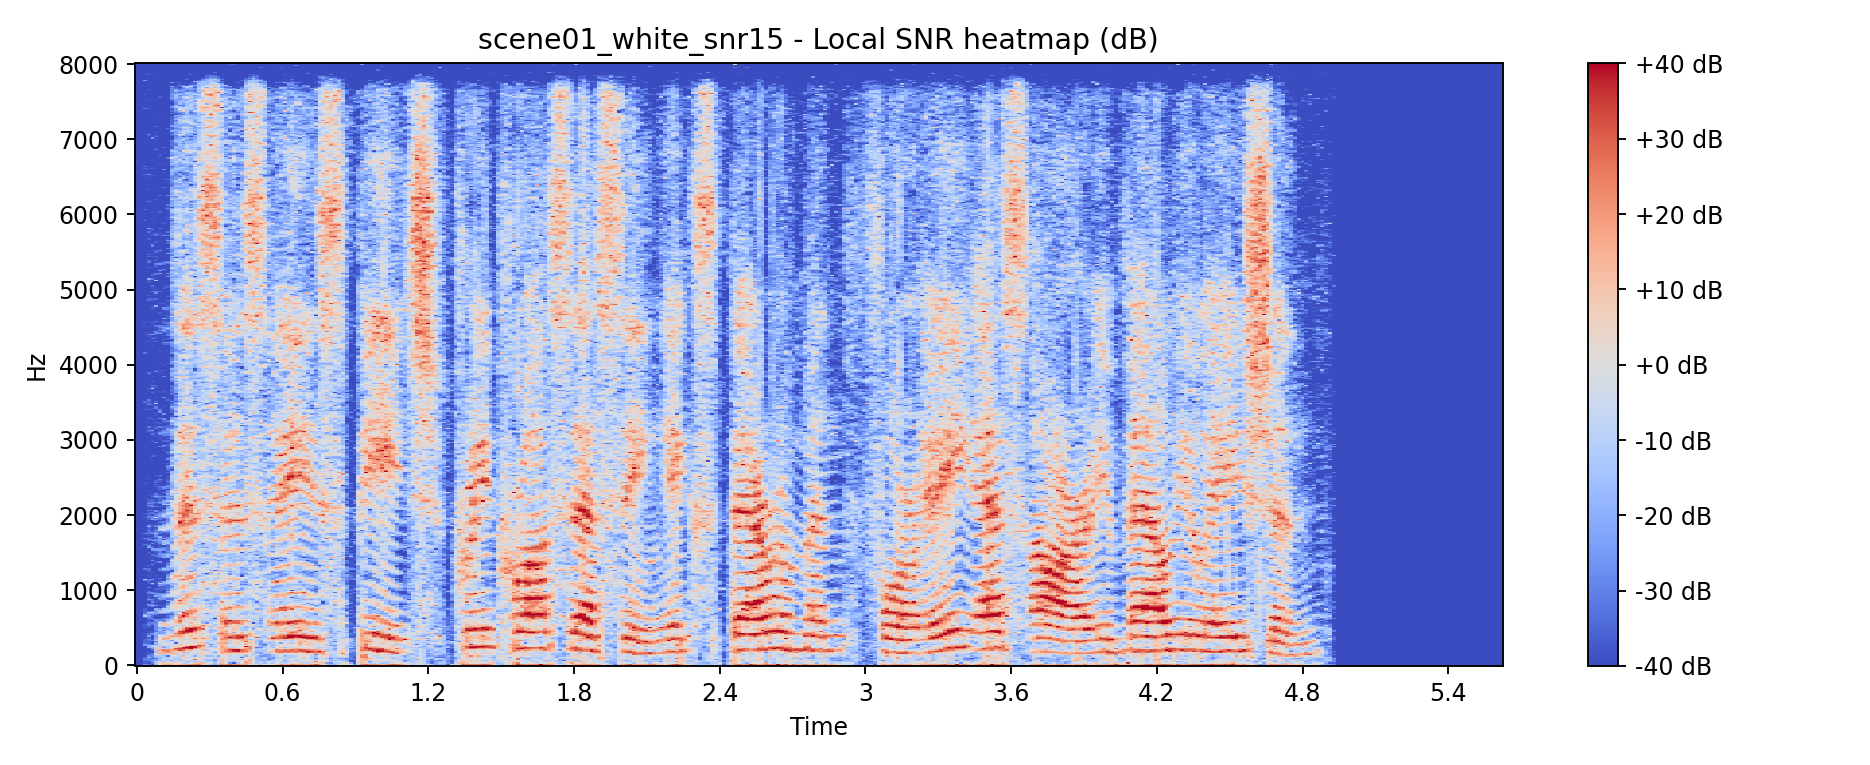
\includegraphics[width=0.6\textwidth]{../analysis/priority_plots/scene01_white_snr15_local_snr_heatmap.png}
  \caption{Local SNR heatmap for \texttt{scene01\_white\_snr15}. Large low-SNR regions explain why fixed spectral subtraction fails.}
  \label{fig:local_snr_heatmap}
\end{figure}

\begin{figure}[H]
  \centering
  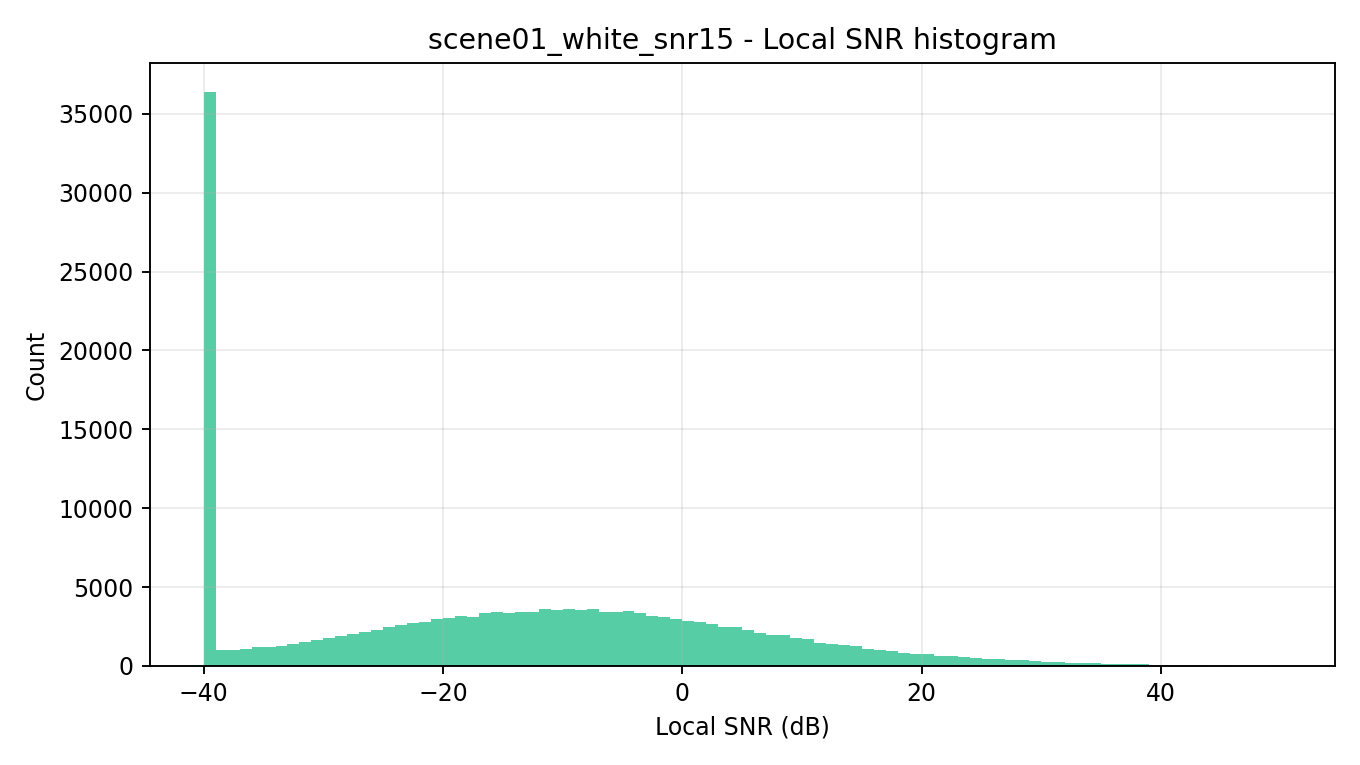
\includegraphics[width=0.6\textwidth]{../analysis/priority_plots/scene01_white_snr15_local_snr_hist.png}
  \caption{Local SNR histogram for scene01. The heavy left tail drives adaptive rather than fixed suppression.}
  \label{fig:local_snr_hist}
\end{figure}

Non-stationarity indices near 0.81--0.83 across white-noise scenes indicate that noise statistics drift over time, supporting recursive noise trackers (MCRA) rather than a single noise profile estimated from the first frames alone.

\section{Feature Separability and Noise Typing}
\label{sec:separability}

\subsection{Cohen's $d$ Effect Sizes}

For each scene, Cohen's $d$ quantifies separability between clean-speech and noise frames in the short-time feature space:
\begin{equation}
  d = \frac{\mu_{\mathrm{clean}} - \mu_{\mathrm{noise}}}
         {\sqrt{(s_{\mathrm{clean}}^2 + s_{\mathrm{noise}}^2)/2}}.
\end{equation}
Values $|d| > 0.8$ indicate large effect sizes. Across the benchmark:

\begin{itemize}
  \item \textbf{ZCR} consistently achieves $|d| > 2$ for broadband noise, making it a reliable VAD auxiliary even when energy $d$ collapses at low SNR.
  \item \textbf{Spectral flatness} maintains $|d| \approx 1.7$ for white/pink scenes, separating harmonic speech from flat noise.
  \item \textbf{Energy} varies widely ($d=0.24$--$0.99$), confirming that energy-only gates are insufficient alone.
\end{itemize}

Structured interference reduces separability differently: chirp scene09 shows lower flatness separability ($d=0.71$) because narrowband energy overlaps speech harmonics, while ZCR separability also drops ($d=1.04$). Such scenes are flagged as \emph{priority optimization} targets requiring specialized modules (subspace projection, chirp notch) rather than generic OM-LSA alone.

\subsection{Automated Noise-Type Labels}

Each scene report assigns a noise-type label stored in JSON metrics, e.g.\
``near-white broadband'' (scene01--02), ``high-frequency dominated'' (scene09 chirp), ``tonal hum'' (scene05--06), or ``reverb + hiss'' (scene15). These labels feed the rule router (\chapref{ch:routing}) alongside numeric features.

\section{ANASS Design Framework}
\label{sec:anass}

ANASS (Adaptive Noise Adaptive Spectral Subtraction) is a three-module design template that maps scene statistics to denoiser parameters. It generalizes classical spectral subtraction by making noise estimation, suppression strength, and artifact control \emph{adaptive in time, frequency, and speech presence}.

\begin{definition}[ANASS Modules]
  \label{def:anass}
  \begin{enumerate}
    \item \textbf{Module 1 --- VAD-gated noise estimation:} estimate noise PSD $\hat{N}(k,t)$ using soft combinations of RMS, ZCR, and spectral flatness rather than hard thresholds.
    \item \textbf{Module 2 --- Adaptive over-subtraction:} apply band- and SNR-dependent oversubtraction factors $\alpha$ and spectral floors $\beta$.
    \item \textbf{Module 3 --- Musical-noise suppression:} reduce bin-wise random peaks via time--frequency smoothing and gain flooring with neighborhood consistency.
  \end{enumerate}
\end{definition}

\subsection{Module 1: VAD-Gated Noise Estimation}

Let $E(t)$, $Z(t)$, and $F(k,t)$ denote frame energy, ZCR, and spectral flatness. A soft speech presence weight for noise updating can be written as
\begin{equation}
  w_{\mathrm{speech}}(t) = \sigma\!\bigl(a_E E_{\mathrm{norm}}(t) + a_Z Z_{\mathrm{norm}}(t) + a_F F_{\mathrm{norm}}(t)\bigr),
  \label{eq:soft_vad}
\end{equation}
where $\sigma(\cdot)$ is a logistic function and normalized features are scaled to $[0,1]$ using scene-dependent percentiles from analysis reports. The noise PSD update rate becomes
\begin{equation}
  \alpha_n(t) = \alpha_{\min} + (1-w_{\mathrm{speech}}(t))\,(\alpha_{\max}-\alpha_{\min}),
\end{equation}
with $\alpha_{\min}, \alpha_{\max}$ drawn from the \texttt{noise\_update} range in Table~\ref{tab:anass_ranges}. Soft gating avoids misclassifying low-energy consonants as noise---a failure mode visible when energy Cohen's $d$ drops below 0.3 (scene02).

In the implemented OM-LSA/MCRA core (\chapref{ch:algorithms}), an equivalent mechanism uses speech presence probability $p_1(k,t)$ per bin rather than frame-level hard VAD.

\subsection{Module 2: Adaptive Over-Subtraction}

Classical magnitude subtraction follows \eqnref{eq:spec_sub} with scalar $\alpha$ and $\beta$. ANASS replaces scalars with band-specific pairs:
\begin{equation}
  \alpha(k) =
  \begin{cases}
    \alpha_{\mathrm{low}}  & f_k < 300\,\mathrm{Hz}, \\
    \alpha_{\mathrm{mid}}  & 300 \le f_k < 3400\,\mathrm{Hz}, \\
    \alpha_{\mathrm{high}} & f_k \ge 3400\,\mathrm{Hz},
  \end{cases}
\end{equation}
and similarly for $\beta(k)$. When high-band SNR falls below mid-band SNR by more than 10\,dB---as in scene01 and scene02---$\alpha_{\mathrm{high}}$ is pushed toward its upper range (3.2--4.0) while $\alpha_{\mathrm{low}}$ remains near 1.4--2.0 to preserve vowel formants.

Local SNR maps further suggest \emph{bin-wise} or \emph{frame-wise} modulation: bins with local SNR${}<0$\,dB receive stronger suppression; bins with local SNR${}>10$\,dB receive near-unity gain. The implemented system approximates this through OM-LSA gains and routing to specialized front-ends rather than explicit per-bin $\alpha$ tables.

\subsection{Module 3: Musical-Noise Suppression}

Fixed subtraction on scene01 yields baseline residual kurtosis $4.38$ and residual flatness 0.203---indicators of heavy-tailed, speckled musical noise. ANASS Module~3 applies:
\begin{itemize}
  \item temporal smoothing coefficient $\in [0.15, 0.35]$ on gain trajectories;
  \item spectral smoothing coefficient $\in [0.05, 0.16]$ across adjacent bins;
  \item a minimum gain floor to prevent isolated deep nulls;
  \item optional neighborhood consistency constraints (implemented in OM-LSA gain-floor blending).
\end{itemize}

High kurtosis ($>4$) in baseline residual reports triggers the upper smoothing range; tonal scenes with low residual kurtosis (e.g., chirp scene09, kurtosis $=2.0$) prioritize structured notch/subspace processing over aggressive smoothing.

\section{Parameter Guidance from Data}
\label{sec:param_guidance}

Table~\ref{tab:anass_ranges} consolidates parameter ranges recommended across all 15 scene reports. Values originate from \texttt{anass\_init\_ranges.json}, derived from pooled local-SNR statistics (median local SNR $\approx -0.62$\,dB; 10th percentile at $-40$\,dB clip) and repeated baseline-subtraction stress tests.

\begin{table}[H]
  \centering
  \caption{Suggested ANASS parameter ranges derived from full-dimensional scene analysis.}
  \label{tab:anass_ranges}
  \begin{tabular}{lcc}
    \toprule
    \textbf{Parameter} & \textbf{Range} & \textbf{Purpose} \\
    \midrule
    $\alpha_{\mathrm{low}}$  & $1.4$--$2.0$   & Speech protection (low/mid band) \\
    $\alpha_{\mathrm{high}}$ & $3.2$--$4.0$   & Stronger suppression (high band) \\
    $\beta_{\mathrm{low}}$   & $0.008$--$0.0176$ & Residual floor (low band) \\
    $\beta_{\mathrm{high}}$  & $0.045$--$0.0765$ & Residual floor (high band) \\
    noise\_update              & $0.87$--$0.93$  & Noise PSD tracking rate \\
    time\_smoothing            & $0.15$--$0.35$  & Temporal artifact reduction \\
    freq\_smoothing            & $0.05$--$0.16$  & Spectral artifact reduction \\
    \bottomrule
  \end{tabular}
\end{table}

\subsection{Representative Scene Snapshots}

Table~\ref{tab:scene_snapshots} contrasts three scenes illustrating how analysis drives different design emphases.

\begin{table}[H]
  \centering
  \caption{Representative scene metrics driving ANASS and routing decisions.}
  \label{tab:scene_snapshots}
  \small
  \begin{tabular}{lccc}
    \toprule
    \textbf{Metric} & \textbf{scene01} & \textbf{scene02} & \textbf{scene09} \\
    \midrule
    Global context      & white, 15\,dB & white, 5\,dB  & chirp, 8\,dB \\
    High-band SNR (dB)  & 1.46          & $-8.50$       & $-4.85$ \\
    Local SNR${}<0$ ratio & 76.7\%     & 89.7\%        & 16.8\% \\
    Energy Cohen's $d$  & 0.99          & 0.24          & 0.56 \\
    Baseline residual kurtosis & 4.38   & 4.57          & 2.00 \\
    ANASS emphasis      & HF $\alpha$, smoothing & strong smoothing, Kalman route & subspace + notch \\
    \bottomrule
  \end{tabular}
\end{table}

\begin{figure}[H]
  \centering
  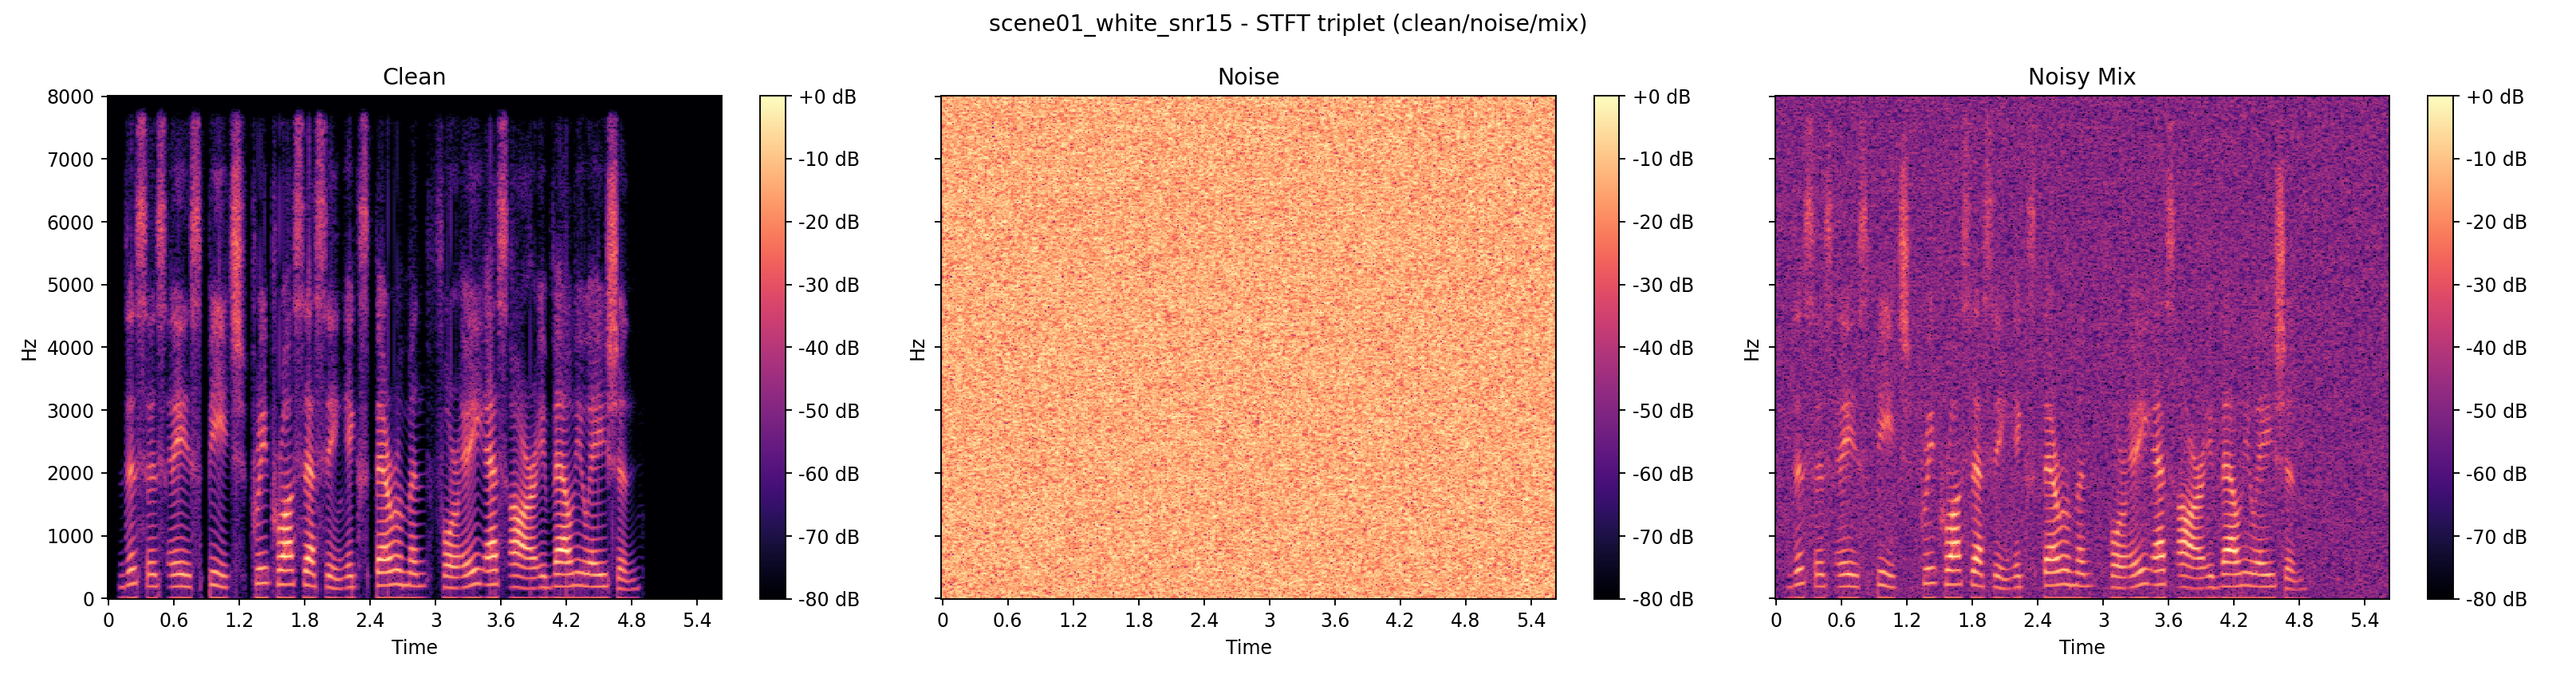
\includegraphics[width=0.92\textwidth]{../analysis/priority_plots/scene01_white_snr15_stft_triplet_clean_noise_mix.png}
  \caption{STFT triplet (clean / noise / mix) for scene01. Visual inspection confirms broadband noise masking high-frequency speech harmonics.}
  \label{fig:stft_triplet}
\end{figure}

\section{Baseline Spectral Subtraction as a Diagnostic Tool}
\label{sec:baseline_diag}

Before deploying adaptive methods, each scene report evaluates fixed-parameter spectral subtraction as a \emph{diagnostic baseline}. Residual metrics predict algorithm bottlenecks:

\begin{itemize}
  \item \textbf{High residual RMS} --- insufficient noise reduction; may need stronger $\alpha$ or specialized front-end.
  \item \textbf{High kurtosis ($>4$)} --- musical-noise risk; Module~3 smoothing required.
  \item \textbf{Elevated residual flatness} --- broadband speckle; check time--frequency smoothing and gain floors.
\end{itemize}

Scene02 baseline residual RMS (0.00805) exceeds scene01 (0.00346) by more than 2$\times$ at lower global SNR, confirming priority for low-SNR optimization and higher distillation training weights (\chapref{ch:dl}).

\section{From Analysis to Implementation}
\label{sec:analysis_to_impl}

The analysis pipeline closes the loop from measurement to deployable configuration in four steps:

\begin{enumerate}
  \item \textbf{Per-scene reports} (\texttt{analysis/reports/}) document domain-specific findings and ANASS recommendations for each WAV file.
  \item \textbf{JSON metrics} (\texttt{analysis/scene\_details/}) expose machine-readable features consumed by \texttt{router/rule\_router.py} for automatic chain selection.
  \item \textbf{Global ranges} (\texttt{anass\_init\_ranges.json}) pool statistics into default parameter intervals for OM-LSA/MCRA tuning.
  \item \textbf{Priority scenarios} flag scenes requiring specialized treatment or heavier distillation weight:
  \begin{itemize}
    \item \texttt{scene12\_babble\_like\_snr5} --- speech-like non-stationary noise;
    \item \texttt{scene10\_impulsive\_clicks\_snr9} --- impulsive outliers;
    \item \texttt{scene09\_chirp\_interference\_snr8} --- narrowband structured interference;
    \item \texttt{scene11\_intermittent\_bursts\_snr7} --- time-varying burst noise.
  \end{itemize}
\end{enumerate}

When \texttt{ratio\_lt0} (fraction of local SNR${}<0$\,dB bins) exceeds 0.75 and mid-band SNR falls below 8\,dB, the router selects \texttt{kalman\_ar} (\chapref{ch:routing}). When high-band SNR${}< -5$\,dB, subspace + OM-LSA chains are preferred. Hum and fan scenes route to adaptive notch filtering based on tonal PSD peaks and noise-type labels.

This data-driven workflow ensures that preprocessing parameters are not chosen arbitrarily: they reflect measurable speech--noise separability, local SNR geography, and predicted failure modes of classical subtraction---directly supporting the ASR preprocessing goal of presenting a cleaner, more stable front-end feature stream (\chapref{ch:introduction}).

\section{Chapter Summary}
\label{sec:scene_summary}

Full-dimensional scene analysis transforms raw noisy recordings into actionable design constraints. Cohen's $d$ separability justifies multi-feature soft VAD; band-wise and local SNR maps motivate frequency-adaptive suppression; baseline residual kurtosis motivates musical-noise control. The ANASS three-module template operationalizes these insights, and the JSON/report artifacts bind analysis to the adaptive router and algorithm library developed in subsequent chapters.

\chapter{Optimized Denoising Algorithms}
\label{ch:algorithms}

This chapter develops the mathematical foundations of the \projectshort{} denoising library. We first formulate single-channel enhancement in the STFT domain, analyze the limitations of fixed-parameter spectral subtraction, and derive the enhanced OM-LSA/MCRA core implemented in \texttt{base\_omlsa\_mcra.py}. We then present six specialized front-end modules and explain why \emph{chainable mixed-algorithm processing}---composition of physics-matched stages followed by a unified OM-LSA back-end---outperforms any single fixed method across heterogeneous noise.

\section{Problem Formulation in the STFT Domain}
\label{sec:stft_formulation}

\subsection{Additive Mixture Model}

The noisy observation is modeled as
\begin{equation}
  y(n) = s(n) + d(n), \quad n = 0,\ldots,N-1,
  \label{eq:time_mix}
\end{equation}
where $s(n)$ is clean speech and $d(n)$ is interference. Speech enhancement seeks an estimate $\hat{s}(n)$ minimizing distortion subject to computational constraints.

\subsection{Short-Time Fourier Analysis}

With Hann window $w(n)$ of length $L=512$, hop $R=128$, and FFT size $L$, the STFT is
\begin{equation}
  Y(k,t) = \sum_{n=0}^{L-1} y(n+tR)\, w(n)\, e^{-j2\pi kn/L},
  \label{eq:stft_def}
\end{equation}
where $k=0,\ldots,L/2$ is the frequency bin and $t$ the frame index. Under the common quasi-stationarity assumption within each frame,
\begin{equation}
  Y(k,t) = S(k,t) + D(k,t).
  \label{eq:stft_mix}
\end{equation}
Enhancement applies a complex gain $\hat{S}(k,t)=G(k,t)\,Y(k,t)$ and synthesizes $\hat{s}(n)$ by overlap-add inverse STFT. With analysis window $w(n)$ and synthesis window $w_s(n)=w(n)$, the COLA reconstruction is
\begin{equation}
  \hat{s}(n) = \frac{\sum_{t\in\mathcal{T}(n)} w_s(n-tR)\, \mathcal{F}^{-1}_L\{\hat{Y}(\cdot,t)\}(n)}
               {\sum_{t\in\mathcal{T}(n)} w_s^2(n-tR) + \varepsilon},
  \label{eq:ola}
\end{equation}
where $\mathcal{F}^{-1}_L\{\cdot\}$ denotes length-$L$ inverse FFT of one-sided bins and $\mathcal{T}(n)=\{t:\,0\le n-tR<L\}$. Project defaults: $L=\texttt{STFT\_NFFT}=512$, $R=\texttt{STFT\_HOP}=128$, Hann window (\texttt{common.py}).

\subsection{Notation and Local SNR}

Instantaneous spectral power and phase are
\begin{align}
  P(k,t) &= |Y(k,t)|^2, \qquad \phi(k,t) = \angle Y(k,t), \\
  \gamma(k,t) &= \frac{P(k,t)}{\mathbb{E}[|D(k,t)|^2] + \varepsilon}, \qquad
  \xi(k,t) = \frac{\mathbb{E}[|S(k,t)|^2]}{\mathbb{E}[|D(k,t)|^2] + \varepsilon},
\end{align}
where $\gamma$ is the \emph{a posteriori} SNR and $\xi$ the \emph{a priori} SNR. Under the distortionless constraint, the MMSE magnitude estimator takes the form $\hat{S}=G(\xi,\gamma)\,Y$ with $0\le G\le 1$.

\begin{table}[H]
  \centering
  \caption{Implementation constants for STFT and OM-LSA/MCRA (\texttt{base\_omlsa\_mcra.py}).}
  \label{tab:omlsa_constants}
  \begin{tabular}{lcl}
    \toprule
    \textbf{Symbol} & \textbf{Value} & \textbf{Role} \\
    \midrule
    $L$, $R$           & 512, 128   & FFT size, hop (75\% overlap) \\
    $\alpha_p$         & 0.8        & Power smoothing for MCRA \\
    $\alpha_{\mathrm{dd}}$ & 0.98   & Decision-directed SNR pole \\
    $\alpha_{\mathrm{noise}}$ & 0.92 & Base noise PSD update \\
    $|\mathcal{W}_t|$  & 30 frames  & Minimum-tracking window ($\approx 240$\,ms) \\
    $T_0$ (init)       & 12 frames  & Initial noise PSD frames \\
    $G_{\mathrm{floor}}$ & 0.06     & Minimum gain (soft floor) \\
    $\varepsilon$      & $10^{-12}$ & Numerical floor \\
    \bottomrule
  \end{tabular}
\end{table}

\subsection{Why Magnitude-Domain Processing}

Human hearing is largely insensitive to phase for narrowband components at moderate SNR; speech intelligibility correlates strongly with short-time \emph{magnitude} envelope structure. The library therefore applies most gains to $|Y(k,t)|$ while retaining the noisy phase $\angle Y(k,t)$ unless a module explicitly modifies the complex spectrum (WPE, chirp cancellation).

\section{Fixed Spectral Subtraction and Its Defects}
\label{sec:fixed_sub_limit}

\subsection{Classical Subtraction}

Given noise magnitude estimate $|\hat{D}(k,t)|$, fixed spectral subtraction sets~\cite{boll1979}
\begin{equation}
  |\tilde{S}(k,t)| = \max\;\Bigl(|Y(k,t)| - \alpha|\hat{D}(k,t)|,\; \beta|Y(k,t)|\Bigr),
  \label{eq:fixed_sub_ch5}
\end{equation}
with scalar $\alpha>1$ (over-subtraction) and floor $\beta\in(0,1)$. Equivalently, in power domain with gain $G=|\tilde{S}|/|Y|$,
\begin{equation}
  G_{\mathrm{sub}}(k,t) = \max\;\left(1 - \alpha\,\frac{\hat{N}(k,t)}{P(k,t)},\; \beta\right),
  \label{eq:sub_gain}
\end{equation}
where $\hat{N}(k,t)\approx \mathbb{E}[|D(k,t)|^2]$. The estimator is \emph{linear in magnitude} and applies independently to each bin.

\subsection{MMSE Benchmark: Wiener and STSA Gains}

For comparison, the Wiener gain under Gaussian spectral coefficients is
\begin{equation}
  G_{\mathrm{W}}(\xi) = \frac{\xi}{1+\xi}.
  \label{eq:wiener_gain}
\end{equation}
The MMSE short-time spectral amplitude (STSA) gain under speech presence hypothesis $H_1$ is~\cite{ephraim1984}
\begin{equation}
  G_{\mathrm{H1}}(\xi,\gamma) = \frac{\xi}{1+\xi}\,\Gamma(0.5)\,\exp\;\Bigl(-\frac{v}{2}\Bigr)\,
  \Bigl[(1+v)I_0\;\Bigl(\frac{v}{2}\Bigr) + v I_1\;\Bigl(\frac{v}{2}\Bigr)\Bigr],
  \label{eq:stsa_gain}
\end{equation}
with $v=\gamma\xi/(1+\xi)$ and modified Bessel functions $I_0,I_1$. OM-LSA replaces \eqref{eq:stsa_gain} by a log-amplitude approximation using the exponential integral $E_1(\cdot)$ (Section~\ref{sec:omlsa_mcra}), yielding smoother low-SNR behavior than \eqref{eq:sub_gain}.

\begin{proposition}[Variance inflation under independent bin subtraction]
\label{prop:musical_noise}
Assume that for a noise-only frame, $|D(k,t)|$ estimates are unbiased and mutually independent across $k$, and subtraction uses a constant $\alpha$. Then the residual magnitude variance $\mathrm{Var}(|\tilde{S}|)$ at bins where $|Y|\approx|\hat{D}|$ scales with the number of independent deep nulls, producing sparse high-variance peaks in time--frequency space (musical noise).
\end{proposition}

\begin{proof}[Sketch]
When $|Y(k,t)|\approx \mathbb{E}|D(k,t)|$, subtraction yields a small positive mean residual but large relative variance because independent estimation errors do not cancel across bins. The ear integrates adjacent frequency channels; isolated random peaks are perceived as tonal artifacts. Scene01 baseline residual kurtosis $4.38$ (\chapref{ch:scene}) quantifies this heavy-tailed residual in practice.
\end{proof}

\subsection{Proposition: Scalar $(\alpha,\beta)$ Cannot Track Local SNR}

\begin{proposition}[Inadequacy of global over-subtraction]
\label{prop:scalar_alpha}
Let $\gamma(k,t)=|Y(k,t)|^2/\mathbb{E}[|D(k,t)|^2]$ be the local a posteriori SNR. A single pair $(\alpha,\beta)$ in \eqref{eq:fixed_sub_ch5} is optimal only if $\gamma(k,t)\equiv \gamma_0$ is constant over all $(k,t)$. For any scene with $\exists (k_1,t_1),(k_2,t_2)$ such that $\gamma(k_1,t_1)\gg \gamma(k_2,t_2)$, either speech at $(k_1,t_1)$ is over-attenuated or noise at $(k_2,t_2)$ is under-suppressed.
\end{proposition}

\begin{proof}
At high $\gamma$, MMSE-optimal gain approaches unity; at low $\gamma$, optimal gain approaches zero. A scalar $\alpha$ selects one compromise slope for all bins. Scene01 exhibits mid-band SNR 18.8\,dB but high-band SNR 1.5\,dB; scene02 high-band SNR is $-8.5$\,dB with 89.7\% of local SNR bins below 0\,dB (\chapref{ch:scene}). No single $(\alpha,\beta)$ can simultaneously protect mid-band vowels and suppress high-band noise.
\end{proof}

These propositions motivate \emph{adaptive, bin-wise, speech-presence-aware} gains---the design principle of OM-LSA/MCRA and the ANASS framework (\chapref{ch:scene}).

\section{Enhanced OM-LSA/MCRA Core}
\label{sec:omlsa_mcra}

The module \texttt{enhance\_spectrum\_omlsa\_mcra} implements a unified pipeline combining (i) MCRA-style noise tracking, (ii) decision-directed a priori SNR estimation, (iii) OM-LSA MMSE log-amplitude gains, and (iv) soft speech-presence blending.

\subsection{Derivation Sketch: From MMSE-STSA to OM-LSA}

Under complex Gaussian models for $S(k,t)$ and $D(k,t)$, the minimum mean-square error estimator of $|S|$ given $|Y|$ under hypothesis $H_1$ (speech present) leads to \eqref{eq:stsa_gain}. Ephraim and Malah show that for low $v$, $G_{\mathrm{H1}}\to 0$ while for large $v$, $G_{\mathrm{H1}}\to \xi/(1+\xi)$. OM-LSA uses the approximation~\cite{ephraim2005}
\begin{equation}
  G_{\mathrm{H1}}^{\mathrm{OM}}(\xi,\gamma) \approx \frac{\xi}{1+\xi}\,
  \exp\;\Bigl(\tfrac{1}{2}\,E_1(v)\Bigr), \quad v = \frac{\gamma\,\xi}{1+\xi},
  \label{eq:omlsa_approx}
\end{equation}
where $E_1(x)=\int_x^{\infty} e^{-t}/t\,dt$. The implementation evaluates \eqref{eq:omlsa_approx} via \texttt{scipy.special.exp1} and clips:
\begin{equation}
  G_{\mathrm{H1}} = \mathrm{clip}\;\bigl(G_{\mathrm{H1}}^{\mathrm{OM}},\, G_{\mathrm{floor}},\, 1\bigr).
  \label{eq:gh1_clip}
\end{equation}

\subsection{MMSE Log-Amplitude Gain (OM-LSA)}

Under a Gaussian complex-spectral model with a priori SNR $\xi(k,t)$ and a posteriori SNR $\gamma(k,t)=|Y|^2/\mathbb{E}[|D|^2]$, the MMSE estimator of the clean magnitude corresponds to a gain~\cite{ephraim1984,ephraim2005}
\begin{equation}
  G_{\mathrm{H1}}(k,t) = \frac{\xi}{1+\xi}\exp\;\Bigl(\tfrac{1}{2}\,E_1(v)\Bigr), \quad
  v = \frac{\gamma\,\xi}{1+\xi},
  \label{eq:omlsa_gain}
\end{equation}
where $E_1(\cdot)$ is the exponential integral. Compared to \eqref{eq:fixed_sub_ch5}, $G_{\mathrm{H1}}$ is a \emph{smooth nonlinear function} of $(\xi,\gamma)$: it approaches $1$ when $\xi\gg 1$ and approaches a frequency-dependent floor when $\xi\to 0$, avoiding hard bin-wise clipping.

\begin{remark}[Advantage over subtraction]
Fixed subtraction applies a linear rule in magnitude; OM-LSA applies a Bayesian shrinkage rule derived from minimum mean-square error estimation. For the same noise PSD estimate, OM-LSA uniformly reduces over-suppression of weak speech components because the gain curve is concave in $\sqrt{\gamma}$ near the origin~\cite{loizou2013}.
\end{remark}

\subsection{Decision-Directed Prior SNR}

Direct estimation $\xi=\max(\gamma-1,0)$ is high-variance at low SNR. The decision-directed (DD) update~\cite{ephraim2005} uses temporal coherence of speech:
\begin{equation}
  \xi(k,t) = \alpha_{\mathrm{dd}}\, G^2(k,t{-}1)\,\gamma(k,t{-}1)
           + (1-\alpha_{\mathrm{dd}})\,\max\bigl(\gamma(k,t)-1,\, 0\bigr),
  \label{eq:dd_prior_snr}
\end{equation}
with $\alpha_{\mathrm{dd}}=0.98$ in our implementation.

\begin{proposition}[Gain-variance reduction via DD smoothing]
\label{prop:dd_variance}
Let $\gamma(k,t)=\gamma_0+\epsilon_t$ where $\epsilon_t$ is zero-mean frame noise with variance $\sigma^2$. For $\alpha_{\mathrm{dd}}$ close to 1, the variance of the DD estimate $\mathrm{Var}(\xi(k,t))$ is reduced by a factor of order $(1-\alpha_{\mathrm{dd}})^2$ relative to the instantaneous estimator $\max(\gamma-1,0)$, at the cost of a bias of order $\alpha_{\mathrm{dd}}$ times the previous-frame mismatch.
\end{proposition}

\begin{proof}[Sketch]
Expand \eqref{eq:dd_prior_snr} as a first-order AR recursion in $\xi$. The innovation term $(1-\alpha_{\mathrm{dd}})\max(\gamma-1,0)$ injects variance $(1-\alpha_{\mathrm{dd}})^2\sigma^2$ per step while the pole at $\alpha_{\mathrm{dd}}$ low-pass filters rapid $\gamma$ fluctuations. Voiced speech maintains correlated $\gamma$ across frames; broadband noise does not, so DD preserves harmonic structure while stabilizing gains---consistent with voiced-frame autocorrelation peaks at lag 96 samples observed in scene analysis.
\end{proof}

\subsection{Speech Presence Probability and Soft Gating}

Define
\begin{equation}
  v(k,t) = \frac{\gamma(k,t)\,\xi(k,t)}{1+\xi(k,t)}, \qquad
  p_1(k,t) = \frac{1}{1+\exp\bigl(-(v(k,t)-1)\bigr)}.
  \label{eq:speech_presence}
\end{equation}
When $v\gg 1$, speech is likely present ($p_1\to 1$); when $v\ll 1$, noise dominates ($p_1\to 0$).

\begin{proposition}[Soft gating dominates hard VAD for mixed frames]
\label{prop:soft_vad}
Let a hard VAD declare ``speech'' iff $v>1$. For frames with $v\approx 1$ (ambiguous low-SNR consonants), hard VAD switches discretely between full noise update and no update, injecting discontinuities in $\hat{N}(k,t)$. Soft weight $p_1(v)$ is Lipschitz-continuous in $v$, bounding the per-frame change in noise PSD update magnitude by $|\partial \hat{N}/\partial p_1|<C$ for some constant $C$ depending on $(P,P_{\min})$.
\end{proposition}

\begin{proof}
Hard VAD replaces $p_1$ with $\mathbb{1}[v>1]$, a discontinuous function. Soft logistic $p_1$ has bounded derivative $|dp_1/dv|\le 1/4$. Since noise update \eqref{eq:noise_update} is affine in $p_0=1-p_1$, gain trajectories are smooth across ambiguous bins---critical when energy Cohen's $d$ falls to 0.24 (scene02) and energy alone cannot gate reliably.
\end{proof}

\subsection{MCRA-Style Adaptive Noise Tracking}

Let $P(k,t)=|Y(k,t)|^2$. Smoothed power and sliding minimum are
\begin{align}
  \bar{P}(k,t) &= \alpha_p \bar{P}(k,t{-}1) + (1-\alpha_p) P(k,t), \\
  P_{\min}(k,t) &= \min_{i\in\mathcal{W}_t} \bar{P}(k,i),
\end{align}
with $\alpha_p=0.8$ and window length $|\mathcal{W}_t|=30$ frames ($\approx 240$\,ms at hop 128, 16\,kHz).

The noise PSD update is
\begin{equation}
  \alpha_t(k) = \alpha_{\mathrm{noise}} + 0.06\, p_1(k,t), \quad \alpha_{\mathrm{noise}}=0.92,
  \label{eq:adaptive_alpha}
\end{equation}
\begin{equation}
  \hat{N}(k,t) = \alpha_t(k)\,\hat{N}(k,t{-}1)
               + \bigl(1-\alpha_t(k)\bigr)\,\bigl(p_0(k,t)\,P(k,t) + (1-p_0(k,t))\,P_{\min}(k,t)\bigr),
  \label{eq:noise_update}
\end{equation}
where $p_0=1-p_1$. The logistic form is a soft surrogate for the speech-presence probability derived from the generalized likelihood ratio in MMSE estimators; the slope at $v=1$ is $1/4$.

Initial noise PSD uses the temporal average of the first $T_0=\min(12,T)$ frames:
\begin{equation}
  \hat{N}(k,0) = \frac{1}{T_0}\sum_{t=0}^{T_0-1} P(k,t).
  \label{eq:noise_init}
\end{equation}

\begin{proposition}[MCRA minimum tracking under non-stationary noise]
\label{prop:mcra}
Suppose that along each frequency bin $k$, there exists at least one frame in every window $\mathcal{W}_t$ where speech power is negligible (silence or noise-only). Then $P_{\min}(k,t)$ is a lower envelope of smoothed power and satisfies $\mathbb{E}[P_{\min}(k,t)] \le \mathbb{E}[|D(k,t)|^2] + \delta$, with bias $\delta$ controlled by window length and $\alpha_p$. Updating $\hat{N}$ toward $P_{\min}$ in noise-dominated bins ($p_0\approx 1$) prevents speech leakage into the noise estimate.
\end{proposition}

\begin{proof}[Sketch]
MCRA~\cite{loizou2013} tracks the minimum of smoothed power because noise-only minima occur during pauses; speech raises the envelope. Weighting by $p_0$ reduces update toward $P$ when $p_1$ is high (speech present) and toward $P_{\min}$ when $p_1$ is low. Non-stationarity index $\approx 0.82$ on white-noise scenes (\chapref{ch:scene}) confirms time-varying noise level, validating recursive tracking over a single static $\hat{N}$.
\end{proof}

\subsection{Soft Gain-Floor Blending}

OM-LSA gain $G_{\mathrm{H1}}$ is blended with floor $G_{\mathrm{floor}}=0.06$:
\begin{equation}
  G(k,t) = G_{\mathrm{H1}}(k,t)^{p_1(k,t)} \cdot G_{\mathrm{floor}}^{\,1-p_1(k,t)}.
  \label{eq:gain_blend}
\end{equation}

\begin{remark}[Physical interpretation]
When $p_1\to 0$ (noise bin), $G\to G_{\mathrm{floor}}$, enforcing a minimum suppression depth equivalent to ANASS $\beta$ flooring (\chapref{ch:scene}). When $p_1\to 1$ (speech bin), $G\to G_{\mathrm{H1}}$, preserving MMSE speech restoration. This implements Module~3 musical-noise control without a separate post-filter: bins uncertain about speech receive intermediate gains, reducing bin-to-bin variance identified in Proposition~\ref{prop:musical_noise}.
\end{remark}

\begin{algorithm}[H]
  \caption{Full OM-LSA/MCRA spectral enhancement (\texttt{enhance\_spectrum\_omlsa\_mcra})}
  \label{alg:omlsa_mcra_full}
  \begin{algorithmic}[1]
    \Require Complex STFT $Y(k,t)$, $k=0\ldots K-1$, $t=0\ldots T-1$; constants Table~\ref{tab:omlsa_constants}
    \Ensure Enhanced spectrum $\hat{Y}(k,t)=G(k,t)Y(k,t)$
    \State $P(k,t) \gets |Y(k,t)|^2$
    \State $T_0 \gets \min(12, T)$;\quad $\hat{N}(k,t) \gets \frac{1}{T_0}\sum_{\tau=0}^{T_0-1} P(k,\tau)$ for all $k,t$ \Comment{init broadcast}
    \State Initialize circular buffer $\mathcal{B}(k,\cdot)$ of length 30 with $\bar{P}(k,0)$
    \State $G(k,-1)\gets 1$;\quad $\gamma(k,-1)\gets 1$ for all $k$
    \For{$t = 0$ \textbf{to} $T-1$}
      \For{$k = 0$ \textbf{to} $K-1$}
        \State $\bar{P}(k,t) \gets \alpha_p \bar{P}(k,t{-}1) + (1-\alpha_p) P(k,t)$
        \State Push $\bar{P}(k,t)$ into $\mathcal{B}$;\quad $P_{\min}(k,t) \gets \min \mathcal{B}(k,\cdot)$
      \EndFor
      \For{$k = 0$ \textbf{to} $K-1$}
        \State $\gamma(k,t) \gets P(k,t) / (\hat{N}(k,t{-}1) + \varepsilon)$
        \If{$t=0$}
          \State $\xi(k,t) \gets \max(\gamma(k,t)-1,\, 0)$
        \Else
          \State $\xi(k,t) \gets \alpha_{\mathrm{dd}} G^2(k,t{-}1)\gamma(k,t{-}1) + (1-\alpha_{\mathrm{dd}})\max(\gamma(k,t)-1,0)$
        \EndIf
        \State $v \gets \gamma\xi/(1+\xi)$;\quad $p_1 \gets 1/(1+\exp(-(v-1)))$;\quad $p_0 \gets 1-p_1$
        \State $\alpha_t \gets \alpha_{\mathrm{noise}} + 0.06\, p_1$
        \State $\hat{N}(k,t) \gets \alpha_t \hat{N}(k,t{-}1) + (1-\alpha_t)(p_0 P + (1-p_0)P_{\min})$
        \State $\gamma(k,t) \gets P(k,t)/(\hat{N}(k,t)+\varepsilon)$
        \State $G_{\mathrm{H1}} \gets \frac{\xi}{1+\xi}\exp(0.5\,E_1(v))$;\quad clip to $[G_{\mathrm{floor}},1]$
        \State $G(k,t) \gets G_{\mathrm{H1}}^{p_1} \cdot G_{\mathrm{floor}}^{(1-p_1)}$
      \EndFor
      \State $\hat{Y}(:,t) \gets G(:,t) \odot Y(:,t)$
    \EndFor
  \end{algorithmic}
\end{algorithm}

\begin{algorithm}[H]
  \caption{Time-domain wrapper \texttt{base\_omlsa\_mcra.process}}
  \label{alg:omlsa_process}
  \begin{algorithmic}[1]
    \Require Noisy waveform $y(n)$, sample rate $f_s$
    \Ensure Enhanced waveform $\hat{s}(n)$
    \State $Y \gets \mathrm{STFT}(y)$ \Comment{$L=512$, $R=128$, Hann}
    \State $\hat{Y} \gets \textsc{EnhanceSpectrumOMLSAMCRA}(Y)$
    \State $\hat{s} \gets \mathrm{iSTFT}(\hat{Y})$ \Comment{Eq.~\eqref{eq:ola}}
    \State \Return $\hat{s}$
  \end{algorithmic}
\end{algorithm}

\section{Physics-Matched Front-End Modules}
\label{sec:modules}

Table~\ref{tab:modules} summarizes six front-end modules. Each targets a distinct physical interference model; all except \texttt{kalman\_ar} (time-domain) operate primarily in STFT or frequency domain before OM-LSA refinement.

\begin{table}[H]
  \centering
  \caption{Denoising modules and physical interference models.}
  \label{tab:modules}
  \begin{tabularx}{\textwidth}{l X l}
    \toprule
    \textbf{Module} & \textbf{Mathematical mechanism} & \textbf{Physical scenario} \\
    \midrule
    \texttt{base\_omlsa\_mcra}     & OM-LSA + MCRA (Section~\ref{sec:omlsa_mcra}) & Broadband stationary noise \\
    \texttt{wpe\_omlsa}            & WPE dereverberation + OM-LSA & Late reverberation + hiss \\
    \texttt{adaptive\_notch\_bank} & IIR notch bank + OM-LSA & Tonal hum / fan harmonics \\
    \texttt{subspace\_denoise}     & SVD subspace projection + OM-LSA & Low-rank colored noise / hiss \\
    \texttt{kalman\_ar}            & AR state-space Kalman + OM-LSA & Low local SNR, speech-like noise \\
    \texttt{nmf\_denoise}          & Semi-supervised NMF + OM-LSA & Mixed noise templates \\
    \texttt{chirp\_notch}          & Ridge tracking + cancellation + OM-LSA & Sweeping narrowband chirp \\
    \bottomrule
  \end{tabularx}
\end{table}

\subsection{Single-Channel WPE + OMLSA (\texttt{wpe\_omlsa})}

\paragraph{Physical model.}
Reverberation convolves speech with room impulse response $h(\tau)$:
\begin{equation}
  y(n) = s(n) + (h * s)(n) + d(n),
\end{equation}
creating spectral coloration and temporal smearing. Weighted Prediction Error (WPE) models late reverberation as predictable from delayed copies of the same STFT bin~\cite{loizou2013}.

\paragraph{Mathematics.}
For each frequency bin $f$, let $y(t)=Y(f,t)$. Late reverberation at frame $t$ is modeled as a linear combination of delayed spectra at the same bin:
\begin{equation}
  y(t) \approx \sum_{k=0}^{K-1} g_k\, y(t-\delta-k-1) + s(t),
  \label{eq:wpe_model}
\end{equation}
with $K=8$ prediction taps and delay $\delta=3$ frames. Define the start index $t_0=\delta+K$ and, for each valid $t\ge t_0$, the prediction matrix
\begin{equation}
  Z_t = \begin{bmatrix}
    y(t-\delta-1) \\ y(t-\delta-2) \\ \vdots \\ y(t-\delta-K)
  \end{bmatrix} \in \mathbb{C}^{K\times 1}.
  \label{eq:wpe_Z}
\end{equation}
Stacking $T'=T-t_0$ columns yields $Z\in\mathbb{C}^{K\times T'}$ and target vector $\mathbf{y}=[y(t_0),\ldots,y(T-1)]^T$. Diagonal WPE~\cite{loizou2013} weights each frame by inverse power $\lambda_t^{-1}=1/\max(|y(t)|^2,\varepsilon)$, giving the weighted normal equations
\begin{align}
  R_f &= \sum_{t=t_0}^{T-1} \lambda_t^{-1}\, Z_t Z_t^H
       = (Z \odot \lambda^{-1/2}) (Z \odot \lambda^{-1/2})^H, \\
  \mathbf{p}_f &= \sum_{t=t_0}^{T-1} \lambda_t^{-1}\, Z_t y^*(t)
              = (Z \odot \lambda^{-1/2}) (\mathbf{y} \odot \lambda^{-1/2})^*, \\
  \mathbf{g}_f &= (R_f + \varepsilon I_K)^{-1} \mathbf{p}_f.
  \label{eq:wpe_normal}
\end{align}
The late-reverberation estimate and dereverberated spectrum are
\begin{equation}
  \hat{L}(f,t) = \mathbf{g}_f^H Z_t, \qquad
  Y^{\mathrm{wpe}}(f,t) = y(t) - \hat{L}(f,t), \quad t\ge t_0.
  \label{eq:wpe_subtract}
\end{equation}
Two outer iterations re-estimate $\mathbf{g}_f$ on the updated $Y^{\mathrm{wpe}}$, refining $\lambda_t$ as power decreases.

\paragraph{Why chain with OM-LSA.}
WPE removes \emph{predictable} spectral components (reflections) but not unpredictable broadband hiss. Denoting WPE output $Y^{\mathrm{wpe}}$, applying OM-LSA estimates $\hat{S}$ from remaining noise:
\begin{equation}
  \hat{S} = G_{\mathrm{OMLSA}}\bigl(|Y^{\mathrm{wpe}}|, \hat{N}\bigr)\, e^{j\angle Y^{\mathrm{wpe}}}.
\end{equation}
This separation-of-concerns is optimal when interference splits into predictable (low-rank in time) plus stochastic residual---matching scene15 (reverb + hiss).

\begin{algorithm}[H]
  \caption{Single-channel WPE in STFT domain (\texttt{single\_channel\_wpe})}
  \label{alg:wpe}
  \begin{algorithmic}[1]
    \Require Complex STFT $Y(f,t)$, taps $K=8$, delay $\delta=3$, iterations $I=2$
    \Ensure Dereverberated STFT $Y^{\mathrm{wpe}}$
    \State $Y^{\mathrm{wpe}} \gets Y$
    \For{$i = 1$ \textbf{to} $I$}
      \For{$f = 0$ \textbf{to} $F-1$}
        \State $y \gets Y^{\mathrm{wpe}}(f,:)$;\quad $t_0 \gets \delta + K$
        \If{$T \le t_0 + 2$} \textbf{continue} \EndIf
        \State Build $Z\in\mathbb{C}^{K\times(T-t_0)}$ with $Z[k,\tau]=y(t_0+\tau-\delta-k-1]$
        \State $\mathbf{y} \gets y[t_0:T-1]$;\quad $\lambda_\tau \gets \max(|y(t_0+\tau)|^2,\varepsilon)$
        \State $R \gets Z \mathrm{diag}(\lambda^{-1}) Z^H$;\quad $\mathbf{p} \gets Z \mathrm{diag}(\lambda^{-1}) \mathbf{y}^*$
        \State $\mathbf{g} \gets \mathrm{solve}(R + \varepsilon I_K,\, \mathbf{p})$ \Comment{fallback: pseudo-inverse}
        \State $\hat{L}(\tau) \gets \mathbf{g}^H Z(:,\tau)$ for all $\tau$
        \State $Y^{\mathrm{wpe}}(f,t_0:T-1) \gets \mathbf{y} - \hat{L}$
      \EndFor
    \EndFor
    \State \Return $Y^{\mathrm{wpe}}$
  \end{algorithmic}
\end{algorithm}

\begin{algorithm}[H]
  \caption{WPE + OM-LSA pipeline (\texttt{wpe\_omlsa.process})}
  \label{alg:wpe_omlsa}
  \begin{algorithmic}[1]
    \Require Waveform $y(n)$, sample rate $f_s$
    \Ensure Enhanced waveform $\hat{s}(n)$
    \State $Y \gets \mathrm{STFT}(y)$
    \State $Y^{\mathrm{wpe}} \gets \textsc{SingleChannelWPE}(Y)$
    \State $\hat{Y} \gets \textsc{EnhanceSpectrumOMLSAMCRA}(Y^{\mathrm{wpe}})$
    \State \Return $\mathrm{iSTFT}(\hat{Y})$
  \end{algorithmic}
\end{algorithm}

\subsection{Adaptive Notch Bank (\texttt{adaptive\_notch\_bank})}

\paragraph{Physical model.}
Power-line hum and fan noise are \emph{narrowband quasi-periodic} tones at $f_0$ and harmonics $hf_0$.

\paragraph{Peak detection.}
Welch PSD $\hat{P}_{\mathrm{welch}}(f)$ with segment length 2048 estimates short-time power. A bin $f_i$ is a tonal peak if it is a local maximum in a 5-point neighborhood and its prominence exceeds 6\,dB:
\begin{equation}
  \mathrm{prom}(f_i) = 10\log_{10}\hat{P}(f_i) - \mathrm{median}\bigl\{10\log_{10}\hat{P}(f_j)\bigr\}_{j\in[i-2,i+2]} > 6\,\mathrm{dB},
  \label{eq:peak_prom}
\end{equation}
subject to $40\,\mathrm{Hz} \le f_i \le \min(0.48 f_s,\, 7800\,\mathrm{Hz})$. Up to eight peaks are retained. Prior harmonics of 50 and 60\,Hz are injected at $hf_0$ for $h=1,\ldots,4$ because grid/fan frequencies are known \emph{a priori}. Nearby peaks within 8\,Hz are merged:
\begin{equation}
  \mathcal{F}_{\mathrm{notch}} = \mathrm{MergeWithin}(\mathcal{F}_{\mathrm{peaks}} \cup \{50h, 60h\},\, 8\,\mathrm{Hz}).
\end{equation}

\paragraph{Notch filtering.}
Each peak $f_0\in\mathcal{F}_{\mathrm{notch}}$ uses a second-order IIR notch with normalized frequency $\omega_0 = 2\pi f_0/f_s$ and quality factor $Q=35$ (below 500\,Hz) or $Q=50$ (above), applied via zero-phase \texttt{filtfilt}:
\begin{equation}
  H(z) = \frac{1 - 2\cos\omega_0\, z^{-1} + z^{-2}}{1 - 2r\cos\omega_0\, z^{-1} + r^2 z^{-2}}, \quad r \approx 1 - \frac{\omega_0}{2Q}.
  \label{eq:notch_tf}
\end{equation}
Cascading notches yields overall transfer $H_{\mathrm{bank}}(z)=\prod_{f_0} H_{f_0}(z)$. Zero-phase filtering applies $H$ forward and backward, squaring magnitude response $|H_{\mathrm{bank}}(e^{j\omega})|^2$ at each tone.

\begin{proposition}[Harmonic energy reduction]
\label{prop:notch}
For a pure tone $A\cos(2\pi f_0 n)$ at bin $f_0$, an ideal notch of width $\Delta f$ attenuates energy in $|f-f_0|<\Delta f/2$ by at least $20\log_{10}(1/\epsilon)$ dB where $\epsilon$ is passband ripple. Cascaded notches at $\{hf_0\}_{h=1}^4$ remove fundamental and low harmonics that broadband OM-LSA treats inefficiently (narrow peaks spread energy across adjacent bins via sidelobe leakage).
\end{proposition}

OM-LSA post-processing removes broadband residual after tonal energy is physically removed---essential for hum50/hum60/fan scenes where tonal SNR dominates.

\begin{algorithm}[H]
  \caption{Adaptive notch bank + OM-LSA (\texttt{adaptive\_notch\_bank})}
  \label{alg:notch_bank}
  \begin{algorithmic}[1]
    \Require Waveform $y(n)$, sample rate $f_s$
    \Ensure Enhanced waveform $\hat{s}(n)$
    \State $\hat{P}(f) \gets \mathrm{Welch}(y,\, n_{\mathrm{seg}}=2048)$
    \State $\mathcal{P} \gets \emptyset$
    \For{each local maximum $f_i$ in $\hat{P}$}
      \If{$\mathrm{prom}(f_i)>6$\,dB and $40\le f_i\le 0.48 f_s$}
        \State $\mathcal{P} \gets \mathcal{P} \cup \{f_i\}$
      \EndIf
    \EndFor
    \State Keep top 8 peaks in $\mathcal{P}$ by prominence
    \State $\mathcal{F} \gets \mathcal{P} \cup \{50h, 60h\}_{h=1..4}$
    \State $\mathcal{F} \gets \mathrm{MergeWithin}(\mathcal{F},\, 8\,\mathrm{Hz})$
    \State $y' \gets y$
    \For{each $f_0 \in \mathcal{F}$}
      \State $Q \gets 35$ if $f_0<500$\,Hz else $50$
      \State $(b,a) \gets \mathrm{iirnotch}(\omega_0=2f_0/f_s,\, Q)$
      \State $y' \gets \mathrm{filtfilt}(b,a,\, y')$ \Comment{zero-phase; Eq.~\eqref{eq:notch_tf}}
    \EndFor
    \State \Return $\textsc{OMLSAProcess}(y')$
  \end{algorithmic}
\end{algorithm}

\subsection{Subspace Denoising (\texttt{subspace\_denoise})}

\paragraph{Physical model.}
Colored noise with low-dimensional spectral structure (hiss concentrated in a subspace spanned by initial frames) occupies a rank-$r$ subspace of magnitude spectrograms.

\paragraph{Mathematics.}
Stack initial $n_0=\min(16,T)$ magnitude frames as matrix $N\in\mathbb{R}^{F\times n_0}$. Thin SVD yields $N = U\Sigma V^T$ with singular values $\sigma_1\ge\cdots\ge\sigma_r$. Noise rank is chosen by cumulative energy:
\begin{equation}
  r = \min\Bigl\{j:\; \frac{\sum_{i=1}^{j}\sigma_i^2}{\sum_{i}\sigma_i^2 + \varepsilon} \ge 0.9\Bigr\}, \quad r \le \min(6,\, \mathrm{rank}(N)).
  \label{eq:subspace_rank}
\end{equation}
Noise subspace basis $U_n = U[:,1:r]$. For full mixture magnitude $M(k,t)=|Y(k,t)|$, orthogonal projection onto the noise subspace and residual are
\begin{align}
  M_n(k,t) &= \sum_{j=1}^{r} \bigl(U_n^T M(:,t)\bigr)_j\, U_n(k,j) = (U_n U_n^T M)(k,t), \\
  M_c(k,t) &= \max\bigl(M(k,t) - M_n(k,t),\, 0\bigr), \\
  G_{\mathrm{sub}}(k,t) &= \mathrm{clip}\;\Bigl(\frac{M_c(k,t)}{M(k,t)+\varepsilon},\, 0.06,\, 1\Bigr).
  \label{eq:subspace_gain}
\end{align}
The complex spectrum is preconditioned as $S_0 = G_{\mathrm{sub}}\odot M \odot e^{j\angle Y}$, then passed to OM-LSA for residual broadband suppression.

\begin{proposition}[Subspace projection error bound]
\label{prop:subspace}
If speech magnitude $S$ lies approximately in subspace orthogonal to $\mathrm{span}(U_n)$ during noise-dominant initialization, then $\|M_n\|_F \approx \|D\|_F$ and $\|M-M_n\|_F \ge \|S\|_F - \epsilon$. When speech subspace overlaps $U_n$ (speech during init), bias $\epsilon$ increases; hence $n_0$ frames are chosen from mixture onset where pauses are likely. High-frequency hiss (scene07) and chirp pre-processing benefit from reducing structured noise rank before OM-LSA.
\end{proposition}

\begin{algorithm}[H]
  \caption{Subspace projection + OM-LSA (\texttt{subspace\_denoise})}
  \label{alg:subspace}
  \begin{algorithmic}[1]
    \Require Waveform $y(n)$, sample rate $f_s$
    \Ensure Enhanced waveform $\hat{s}(n)$
    \State $Y \gets \mathrm{STFT}(y)$;\quad $M \gets |Y|$;\quad $\Phi \gets e^{j\angle Y}$
    \State $N \gets M(:, 0:n_0-1)$ with $n_0=\min(16,T)$
    \State $U,\Sigma,V^T \gets \mathrm{SVD}(N)$
    \State $r \gets \mathrm{RankByEnergy}(\Sigma,\, 0.9)$ clipped to $[1,\min(6,\mathrm{rank})]$ \Comment{Eq.~\eqref{eq:subspace_rank}}
    \State $U_n \gets U(:,1:r)$
    \State $M_n \gets U_n (U_n^T M)$;\quad $M_c \gets \max(M - M_n, 0)$
    \State $G \gets \mathrm{clip}(M_c/(M+\varepsilon),\, 0.06,\, 1)$
    \State $S_0 \gets G \odot M \odot \Phi$
    \State $\hat{Y} \gets \textsc{EnhanceSpectrumOMLSAMCRA}(S_0)$
    \State \Return $\mathrm{iSTFT}(\hat{Y})$
  \end{algorithmic}
\end{algorithm}

\subsection{Kalman--AR Filtering (\texttt{kalman\_ar})}

\paragraph{Physical model.}
Voiced speech is strongly predictable by linear prediction; babble and low-SNR noise are less predictable by low-order AR models.

\paragraph{Yule--Walker AR($p$).}
Sample autocorrelation $r(\ell)=\sum_n y(n)y(n+\ell)$ yields Toeplitz system for AR coefficients $\mathbf{a}=[a_1,\ldots,a_p]^T$ with order $p=10$:
\begin{equation}
  \sum_{k=1}^{p} a_k\, r(|i-k|) = r(i+1), \quad i=0,\ldots,p-1
  \quad \Leftrightarrow \quad R\mathbf{a}=\mathbf{r},
  \label{eq:yule_walker}
\end{equation}
where $R_{ij}=r(|i-j|)$ and $r_i=r(i+1)$. Tikhonov regularization $R+\varepsilon I$ stabilizes ill-conditioned segments.

\paragraph{State-space model.}
State $\mathbf{x}_k = [s_k, s_{k-1},\ldots,s_{k-p+1}]^T$ evolves as
\begin{equation}
  \mathbf{x}_{k+1} = F\mathbf{x}_k + \mathbf{w}_k, \quad y_k = H\mathbf{x}_k + v_k,
  \label{eq:kalman_ss}
\end{equation}
with companion matrix
\begin{equation}
  F = \begin{bmatrix}
    a_1 & a_2 & \cdots & a_p \\
    1   & 0   & \cdots & 0 \\
    0   & 1   & \ddots & \vdots \\
    0   & 0   & \cdots & 0
  \end{bmatrix}, \quad H=[1,0,\ldots,0],
\end{equation}
process noise $\mathbf{w}_k\sim\mathcal{N}(0,Q)$ with $Q=\sigma_p^2 I_p$, $\sigma_p^2=0.2\,\hat{\sigma}_y^2$, and observation noise $v_k\sim\mathcal{N}(0,R)$, $R=\hat{\sigma}_y^2$, where $\hat{\sigma}_y^2=\mathrm{Var}(y[0:2000])$.

\paragraph{Kalman recursion.}
At each sample $k$, predict then update:
\begin{align}
  \hat{\mathbf{x}}_{k|k-1} &= F\hat{\mathbf{x}}_{k-1|k-1}, &
  P_{k|k-1} &= F P_{k-1|k-1} F^T + Q, \\
  K_k &= P_{k|k-1} H^T (H P_{k|k-1} H^T + R)^{-1}, \\
  \hat{\mathbf{x}}_{k|k} &= \hat{\mathbf{x}}_{k|k-1} + K_k (y_k - H\hat{\mathbf{x}}_{k|k-1}), &
  P_{k|k} &= (I - K_k H) P_{k|k-1}.
  \label{eq:kalman_update}
\end{align}
The filtered speech estimate is $\hat{s}_k = (\hat{\mathbf{x}}_{k|k})_1$.

\begin{proposition}[MMSE linear prediction advantage at low SNR]
\label{prop:kalman}
When $s_k$ is AR($p$)-predictable and $d_k$ is white with variance $\sigma_d^2$, the Kalman smoother attenuates components of $y_k$ uncorrelated with the AR subspace. For local SNR $\ll 0$\,dB (89.7\% bins in scene02), linear MMSE estimation reduces noise variance before nonlinear OM-LSA, improving effective $\gamma(k,t)$ in subsequent STFT processing.
\end{proposition}

\begin{algorithm}[H]
  \caption{Kalman--AR filter + OM-LSA (\texttt{kalman\_ar})}
  \label{alg:kalman_ar}
  \begin{algorithmic}[1]
    \Require Waveform $y(n)$, AR order $p=10$, sample rate $f_s$
    \Ensure Enhanced waveform $\hat{s}(n)$
    \State $\mathbf{a} \gets \mathrm{YuleWalkerAR}(y,\, p)$ \Comment{solve \eqref{eq:yule_walker}}
    \State Build $F,H$ from $\mathbf{a}$;\quad $\hat{\sigma}^2 \gets \mathrm{Var}(y[0:2000])$
    \State $Q \gets 0.2\hat{\sigma}^2 I_p$;\quad $R \gets \hat{\sigma}^2$
    \State $\hat{\mathbf{x}} \gets \mathbf{0}$;\quad $P \gets I_p$
    \For{$k = 0$ \textbf{to} $N-1$}
      \State $\hat{\mathbf{x}}^- \gets F\hat{\mathbf{x}}$;\quad $P^- \gets F P F^T + Q$
      \State $K \gets P^- H^T (H P^- H^T + R)^{-1}$ \Comment{\eqref{eq:kalman_update}}
      \State $\hat{\mathbf{x}} \gets \hat{\mathbf{x}}^- + K(y_k - H\hat{\mathbf{x}}^-)$
      \State $P \gets (I - K H) P^-$;\quad $\hat{s}_k \gets \hat{x}_1$
    \EndFor
    \State \Return $\textsc{OMLSAProcess}(\hat{s})$
  \end{algorithmic}
\end{algorithm}

\subsection{NMF Denoising (\texttt{nmf\_denoise})}

\paragraph{Physical model.}
Magnitude spectrograms are approximately low-rank non-negative matrices $V\approx WH$ with speech and noise bases.

\paragraph{Mathematics.}
Magnitude spectrogram $V\in\mathbb{R}^{F\times T}_+$ is approximated by non-negative matrix factorization $V\approx WH$ with $W\in\mathbb{R}^{F\times r}_+$, $H\in\mathbb{R}^{r\times T}_+$. We minimize KL divergence
\begin{equation}
  D_{\mathrm{KL}}(V\|WH) = \sum_{f,t}\Bigl(V_{ft}\log\frac{V_{ft}}{(WH)_{ft}} - V_{ft} + (WH)_{ft}\Bigr),
  \label{eq:nmf_kl}
\end{equation}
via multiplicative updates (MU)~\cite{lee1999}:
\begin{equation}
  H \leftarrow H \odot \frac{W^T(V \oslash WH)}{W^T \mathbf{1} + \varepsilon}, \quad
  W \leftarrow W \odot \frac{(V \oslash WH)H^T}{\mathbf{1}H^T + \varepsilon},
  \label{eq:nmf_mu}
\end{equation}
where $\oslash$ denotes element-wise division and $\odot$ element-wise product. Columns of $W$ are column-normalized after each $W$-update.

\paragraph{Semi-supervised template split.}
From initial $n_0=\min(12,T)$ noise frames $V_n=V(:,0:n_0-1)$ and speech frames $V_s=V(:,n_0:)$, learn separate dictionaries:
\begin{equation}
  W_n\in\mathbb{R}^{F\times 4}_+ \text{ from } V_n \text{ (30 MU iters)}, \quad
  W_s\in\mathbb{R}^{F\times 8}_+ \text{ from } V_s \text{ (40 MU iters)}.
\end{equation}
Concatenate $W=[W_s,\, W_n]\in\mathbb{R}^{F\times 12}_+$ and refine activations $H$ on the full $V$ for 60 iterations with $W$ fixed. Split $H=[H_s^T,H_n^T]^T$ and reconstruct
\begin{equation}
  V_s = W_s H_s, \quad V_n = W_n H_n, \quad
  G(k,t) = \mathrm{clip}\;\Bigl(\frac{V_s}{V_s + V_n + \varepsilon},\, 0.05,\, 1\Bigr).
  \label{eq:nmf_gain}
\end{equation}
Apply $S_0 = G\odot V \odot e^{j\angle Y}$ followed by OM-LSA.

\begin{remark}
NMF separates \emph{templates} (spectral shapes) from activations (time). After notch removal of tones, residual fan noise with stable spectral shape is well modeled by $W_n$, while speech uses $W_s$---motivating \texttt{adaptive\_notch\_bank} $\rightarrow$ \texttt{nmf\_denoise} chains.
\end{remark}

\begin{algorithm}[H]
  \caption{Semi-supervised NMF + OM-LSA (\texttt{nmf\_denoise})}
  \label{alg:nmf}
  \begin{algorithmic}[1]
    \Require Waveform $y(n)$, sample rate $f_s$
    \Ensure Enhanced waveform $\hat{s}(n)$
    \State $Y \gets \mathrm{STFT}(y)$;\quad $V \gets |Y|$;\quad $\Phi \gets e^{j\angle Y}$
    \State $n_0 \gets \min(12,T)$;\quad $V_n \gets V(:,0:n_0-1)$;\quad $V_s \gets V(:,n_0:)$ (or $V$ if $T\le n_0$)
    \State $W_n \gets \mathrm{NMF\_MU}(V_n,\, r=4,\, \mathrm{iters}=30)$
    \State $W_s \gets \mathrm{NMF\_MU}(V_s,\, r=8,\, \mathrm{iters}=40)$
    \State $W \gets [W_s,\, W_n]$;\quad initialize $H\in\mathbb{R}^{12\times T}_+$
    \For{$i=1$ \textbf{to} $60$} \Comment{fix $W$, update $H$ only}
      \State $H \gets H \odot \dfrac{W^T(V \oslash WH)}{W^T\mathbf{1}+\varepsilon}$ \Comment{\eqref{eq:nmf_mu}}
    \EndFor
    \State $H_s \gets H[1:8,:]$;\quad $H_n \gets H[9:12,:]$
    \State $V_s \gets W_s H_s$;\quad $V_n \gets W_n H_n$
    \State $G \gets \mathrm{clip}(V_s/(V_s+V_n+\varepsilon),\, 0.05,\, 1)$
    \State $S_0 \gets G \odot V \odot \Phi$
    \State \Return $\mathrm{iSTFT}(\textsc{EnhanceSpectrumOMLSAMCRA}(S_0))$
  \end{algorithmic}
\end{algorithm}

\subsection{Chirp Notch (\texttt{chirp\_notch})}

\paragraph{Physical model.}
Chirp interference is a narrowband component whose center frequency $f_c(t)$ sweeps in time, visible as a ridge in spectrograms (scene09).

\paragraph{Ridge tracking.}
Let $M(k,t)=|Y(k,t)|$ and $M_{\mathrm{dB}}=20\log_{10}(M+\varepsilon)$. Restrict search to high-band bins $\mathcal{K}=\{k: f_k\ge 700\,\mathrm{Hz}\}$. Per frame $t$, candidate ridge bin is
\begin{equation}
  k_c(t) = \arg\max_{k\in\mathcal{K}} M_{\mathrm{dB}}(k,t),
\end{equation}
with prominence $p(t)=M_{\mathrm{dB}}(k_c,t)-\mathrm{median}\{M_{\mathrm{dB}}(k,t)\}_{k\in\mathcal{K}}$. Spectral flatness in the band validates narrowband structure:
\begin{equation}
  \mathrm{SF}(t) = \frac{\exp\bigl(\frac{1}{|\mathcal{K}|}\sum_{k\in\mathcal{K}}\log M(k,t)\bigr)}{\frac{1}{|\mathcal{K}|}\sum_{k\in\mathcal{K}} M(k,t)}.
  \label{eq:spec_flat}
\end{equation}
Acceptance requires $(p>10\,\mathrm{dB} \land \mathrm{SF}<0.18)$ below 1.5\,kHz, or $(p>8\,\mathrm{dB} \land \mathrm{SF}<0.25)$ above; large frame-to-frame jumps $|k_c(t)-k_c(t-1)|>10$ require $p>15$\,dB. Valid frames are linearly interpolated, then median-filtered (kernel 9) to obtain smooth track $\tilde{k}_c(t)$.

\paragraph{Stage 1: complex-domain cancellation.}
Gaussian weights $w_k=\exp\bigl(-\tfrac{1}{2}((k-k_c)/\sigma_k)^2\bigr)$ with $\sigma_k\in[1.4,2.2]$ depend on prominence. Cancellation strength $\beta\in[0.55,0.95]$ scales with $p(t)$. Frequency protection $p(f)<1$ below 1.8\,kHz preserves formants:
\begin{equation}
  Y'(k,t) = Y(k,t) - \beta(t)\, p(f_k)\, w_k(k-k_c(t))\, Y(k,t).
  \label{eq:chirp_cancel}
\end{equation}

\paragraph{Stage 2--4: OM-LSA, Gaussian notch, inpainting.}
OM-LSA is applied to $Y'$. A time-varying mask attenuates residual ridge energy:
\begin{equation}
  M_{\mathrm{notch}}(k,t) = \mathrm{clip}\;\Bigl(1 - 0.9\, d(t)\, e^{-\frac{1}{2}\left(\frac{k-k_c(t)}{\sigma_n(t)}\right)^2},\, 0.06,\, 1\Bigr),
\end{equation}
with depth $d(t)=\mathrm{clip}((p(t)-8)/12,\,0,1)$. Temporal smoothing applies $0.2\,M_{t-1}+0.6\,M_t+0.2\,M_{t+1}$. Finally, ridge magnitude is inpainted from medians of neighboring off-ridge bins:
\begin{equation}
  |\hat{Y}(k,t)| = \mathrm{median}\bigl\{M(k',t): k'\in [k_c-w,\, k_c+w]^c\bigr\}, \quad |k-k_c|\le w.
  \label{eq:chirp_inpaint}
\end{equation}

\begin{proposition}[Why OM-LSA alone fails on chirp]
\label{prop:chirp}
OM-LSA assumes slowly varying noise PSD per bin. A chirp violates this: energy migrates across bins, so $\hat{N}(k,t)$ cannot track a moving ridge. Explicit ridge cancellation removes \emph{non-stationary narrowband} structure that violates MCRA assumptions, restoring validity of Proposition~\ref{prop:mcra} on the residual.
\end{proposition}

\begin{algorithm}[H]
  \caption{Four-stage chirp suppression (\texttt{chirp\_notch})}
  \label{alg:chirp}
  \begin{algorithmic}[1]
    \Require Waveform $y(n)$, sample rate $f_s$
    \Ensure Enhanced waveform $\hat{s}(n)$
    \State $Y \gets \mathrm{STFT}(y)$;\quad $\{f_k\} \gets$ frequency axis
    \State $(k_c, p) \gets \textsc{DetectChirpTrack}(Y, f_k)$ \Comment{Eqs.~\eqref{eq:spec_flat}, prominence gates}
    \State $Y_1 \gets \textsc{CancelChirpComponent}(Y, k_c, p)$ \Comment{Eq.~\eqref{eq:chirp_cancel}}
    \State $Y_2 \gets \textsc{EnhanceSpectrumOMLSAMCRA}(Y_1)$
    \State $Y_3 \gets \textsc{ApplyChirpNotchMask}(Y_2, k_c, p)$
    \State $\hat{Y} \gets \textsc{InpaintRidgeMag}(Y_3, k_c, p)$ \Comment{Eq.~\eqref{eq:chirp_inpaint}}
    \State \Return $\mathrm{iSTFT}(\hat{Y})$
  \end{algorithmic}
\end{algorithm}

\section{Chainable Mixed-Algorithm Processing}
\label{sec:chains}

\subsection{Composition Operator}

Let $\Phi_i$ denote the STFT-domain enhancement operator of stage $i$, so $\hat{Y}=\Phi_m\circ\cdots\circ\Phi_1(Y)$. The library implements chains via \texttt{apply\_chain} in \texttt{common.py}:
\begin{equation}
  \hat{s} = \mathcal{T}^{-1}\bigl(\Phi_m \circ \cdots \circ \Phi_1(\mathcal{T}y)\bigr),
\end{equation}
where $\mathcal{T}$ is STFT and $\mathcal{T}^{-1}$ is overlap-add synthesis. In practice each $\Phi_i$ is a time-domain module $f_i(y,f_s)$ that may internally perform its own STFT/iSTFT; composition is sequential:
\begin{equation}
  y^{(0)}=y, \quad y^{(i)}=f_i(y^{(i-1)}, f_s),\quad i=1,\ldots,m, \quad \hat{s}=y^{(m)}.
  \label{eq:chain_compose}
\end{equation}

\begin{algorithm}[H]
  \caption{Mixed-algorithm chain execution (\texttt{apply\_chain})}
  \label{alg:apply_chain}
  \begin{algorithmic}[1]
    \Require Waveform $y(n)$, sample rate $f_s$, ordered list of processors $\{f_1,\ldots,f_m\}$
    \Ensure Enhanced waveform $\hat{s}(n)$
    \State $y' \gets y$
    \For{$i = 1$ \textbf{to} $m$}
      \State $y' \gets f_i(y',\, f_s)$ \Comment{Eq.~\eqref{eq:chain_compose}}
    \EndFor
    \State \Return $y'$
  \end{algorithmic}
\end{algorithm}

\begin{definition}[Physics-matched decomposition]
\label{def:physics_match}
Interference $d(n)$ admits a physics-matched decomposition if
\begin{equation}
  d(n) = d^{(1)}(n) + d^{(2)}(n) + \cdots + d^{(m)}(n),
\end{equation}
where each $d^{(i)}$ is the perturbation class targeted by $\Phi_i$ (tonal, reverberation, chirp, broadband, etc.).
\end{definition}

\subsection{Theorem: Sequential Reduction of Structured Components}

\begin{theorem}[Structured-interference reduction]
\label{thm:chain}
Suppose $Y=S+D^{(1)}+D^{(2)}+W$ where $\Phi_1$ removes $D^{(1)}$ with attenuation $A_1>0$\,dB in its subspace, and $\Phi_2$ is OM-LSA designed for stochastic residual $D^{(2)}+W$. If $\Phi_1$ is approximately linear on $D^{(1)}$ and orthogonal to $S$ in mean-square sense, then the post-chain a posteriori SNR satisfies
\begin{equation}
  \gamma_{\mathrm{post}} \ge \gamma_{\mathrm{omlsa-only}} + \Delta(A_1),
\end{equation}
where $\Delta(A_1)>0$ increases with tonal/reverberation energy removed before OM-LSA.
\end{theorem}

\begin{proof}[Sketch]
OM-LSA gain is monotonic in $\gamma$. Removing $D^{(1)}$ before OM-LSA lowers effective noise power in affected bins, increasing $\gamma(k,t)$ for fixed $|S|$. For hum tones, notch attenuation of 20--40\,dB at harmonics directly increases local SNR in those bins. For chirp, ridge cancellation prevents energy smearing that inflates $\hat{N}$ across bins. Empirically, scene09 chirp chain (\texttt{subspace\_denoise} $\rightarrow$ \texttt{chirp\_notch}) reduces distill-refinement RMS error by 0.0019 versus routed-only (\chapref{ch:experiments}).
\end{proof}

\subsection{Canonical Chains in \projectshort{}}

\begin{table}[H]
  \centering
  \caption{Physics-matched algorithm chains used by the rule router.}
  \label{tab:chains}
  \begin{tabular}{lll}
    \toprule
    \textbf{Chain} & \textbf{Stages} & \textbf{Rationale (Theorem~\ref{thm:chain})} \\
    \midrule
    Hum / fan   & notch $\rightarrow$ NMF $\rightarrow$ OM-LSA & Remove tones, separate templates, suppress residual \\
    Chirp       & subspace $\rightarrow$ chirp notch & Reduce rank, cancel moving ridge, OM-LSA inside chirp module \\
    Reverb+hiss & WPE $\rightarrow$ OM-LSA & Predictable late reverb then stochastic hiss \\
    Low SNR     & Kalman AR $\rightarrow$ OM-LSA & Linear speech subspace then broadband \\
    Hiss-heavy  & subspace $\rightarrow$ OM-LSA & Low-rank noise then MMSE \\
    Default     & OM-LSA/MCRA only & Broadband near-stationary noise \\
    \bottomrule
  \end{tabular}
\end{table}

\subsection{Why a Unified OM-LSA Back-End}

Using one OM-LSA/MCRA implementation as the final stage ensures:
\begin{enumerate}
  \item \textbf{Consistent gain physics} --- all paths apply MMSE shrinkage and soft flooring (Propositions~\ref{prop:soft_vad}--\ref{prop:mcra}).
  \item \textbf{Parameter portability} --- ANASS ranges (\chapref{ch:scene}) tune a single back-end.
  \item \textbf{Distillation compatibility} --- TinyResidualRefiner learns residual masks on a consistent routed STFT statistics (\chapref{ch:dl}).
\end{enumerate}

Front-ends linearly or nonlinearly \emph{precondition} the mixture so that OM-LSA assumptions (slowly varying $\hat{N}$, speech sparsity in time-frequency) hold more closely---this is the central advantage of mixed-algorithm processing over monolithic fixed subtraction or a single undifferentiated OM-LSA instance.

\section{Comparison Summary}
\label{sec:algo_comparison}

\begin{table}[H]
  \centering
  \caption{Qualitative comparison: fixed subtraction vs.\ adaptive OM-LSA vs.\ mixed chains.}
  \label{tab:algo_compare}
  \small
  \begin{tabular}{lccc}
    \toprule
    \textbf{Criterion} & \textbf{Fixed subtract.} & \textbf{OM-LSA/MCRA} & \textbf{Mixed chain} \\
    \midrule
    Local SNR adaptivity       & No  & Yes (bin-wise) & Yes + structural \\
    Non-stationary noise       & Poor & Good (MCRA)   & Excellent \\
    Tonal / chirp interference & Poor & Poor          & Excellent \\
    Reverberation              & Poor & Moderate      & Good (WPE) \\
    Interpretability           & High & High          & High (logged chain) \\
    Compute cost               & Low  & Low           & Low--medium \\
    \bottomrule
  \end{tabular}
\end{table}

\section{Chapter Summary}
\label{sec:algo_summary}

The enhanced OM-LSA/MCRA core replaces scalar spectral subtraction with MMSE Bayesian gains, decision-directed SNR smoothing, MCRA noise tracking, and logistic speech-presence blending---addressing Propositions~\ref{prop:musical_noise}--\ref{prop:scalar_alpha}. Specialized modules attack interference classes that violate OM-LSA assumptions: tonal hum (notches), reverberation (WPE), low-rank hiss (subspace), low local SNR (Kalman--AR), mixed templates (NMF), and sweeping chirp (ridge cancellation). Theorem~\ref{thm:chain} formalizes why sequential physics-matched composition with a unified OM-LSA back-end yields lower residual error than any single algorithm on heterogeneous scenes. \chapref{ch:routing} describes how scene metrics select among these chains automatically.

\chapter{Adaptive Routing Mechanism}
\label{ch:routing}

Chapter~\chapref{ch:algorithms} established that heterogeneous interference requires \emph{physics-matched algorithm chains} rather than a single fixed enhancer. Chapter~\chapref{ch:scene} showed that global SNR and noise labels alone are insufficient: band-wise imbalance, local SNR tails, and separability statistics differ sharply across the 15 benchmark scenes. This chapter describes how \projectshort{} closes the loop between offline scene analysis and online denoising selection through a transparent, priority-ordered rule router (\texttt{router/rule\_router.py}), optional evaluation-driven overrides, and auditable chain execution in both CLI and web pipelines.

\section{Motivation for Scene-Aware Routing}
\label{sec:routing_motivation}

\subsection{Why One Algorithm Is Not Enough}

Fixed-parameter spectral subtraction fails when local SNR varies across time and frequency (Propositions~\ref{prop:musical_noise}--\ref{prop:scalar_alpha}, \chapref{ch:algorithms}). Even adaptive OM-LSA/MCRA assumes slowly varying noise PSD per bin; tonal hum, sweeping chirp, late reverberation, and speech-like babble violate distinct subsets of these assumptions (Propositions~\ref{prop:notch}--\ref{prop:chirp}). Theorem~\ref{thm:chain} formalizes the benefit of sequential, physics-matched composition: remove structured interference \emph{first}, then apply the unified OM-LSA back-end on a better-conditioned residual.

A practical platform therefore needs a \emph{routing layer} that maps each incoming scene to an algorithm chain $\mathcal{C}=\{f_1,\ldots,f_m\}$ drawn from the method registry, without requiring the end user to inspect spectrograms or tune seven modules manually.

\subsection{Design Goals}

The routing mechanism in \projectshort{} is deliberately rule-based rather than learned, for four reasons aligned with the project research questions:
\begin{enumerate}
  \item \textbf{Interpretability} --- every decision exposes a human-readable \texttt{reason} string and named \texttt{route\_name}, supporting failure analysis and report writing.
  \item \textbf{Traceability to analysis} --- rules consume the same JSON metrics produced by full-dimensional scene analysis (\chapref{ch:scene}), linking measurement to action.
  \item \textbf{Low latency} --- routing is $O(1)$ JSON lookup plus a short conditional chain; no neural inference is required at route time.
  \item \textbf{Extensibility} --- new scenes, thresholds, or chains can be added without retraining; grid-search overrides provide a data-driven refinement path when rules are suboptimal.
\end{enumerate}

\section{Router Architecture}
\label{sec:router_arch}

\subsection{RouteDecision Object}

The router returns a \texttt{RouteDecision} dataclass with three fields:
\begin{itemize}
  \item \texttt{route\_name} --- canonical label (e.g., \texttt{hum\_stationary\_chain}, \texttt{base\_chain});
  \item \texttt{chain} --- ordered list of method keys executed sequentially;
  \item \texttt{reason} --- short audit string stored in \texttt{route\_log.json} and returned by the web API.
\end{itemize}

Chain execution follows Eq.~\eqref{eq:chain_compose}: each stage receives the waveform output of the previous stage at the same sample rate $f_s$.

\subsection{Decision Priority}

Routing applies decisions in strict priority order:
\begin{enumerate}
  \item \textbf{CLI force} --- \texttt{--force-method} (batch) or explicit method in the web UI bypasses all rules;
  \item \textbf{Config override} --- per-scene entry in \texttt{scene\_method\_overrides.json};
  \item \textbf{Metric and keyword rules} --- \texttt{choose\_route()} conditional tree;
  \item \textbf{Default fallback} --- single-stage \texttt{base\_omlsa\_mcra}.
\end{enumerate}


\section{Routing Feature Vector}
\label{sec:routing_features}

\subsection{Metrics Input}

For scene filename $s$ (e.g., \texttt{scene07\_highfreq\_hiss\_snr10.wav}), the router loads
\begin{equation}
  \mathcal{M}(s) = \text{JSON}\bigl(\texttt{analysis/scene\_details/}\,\mathrm{stem}(s)\,\texttt{\_metrics.json}\bigr),
\end{equation}
or the empty dict if the file is missing. Five scalar features drive automatic rules (Table~\ref{tab:routing_features}).

\begin{table}[H]
  \centering
  \caption{Routing features extracted from per-scene metrics JSON.}
  \label{tab:routing_features}
  \small
  \begin{tabularx}{\textwidth}{l l X}
    \toprule
    \textbf{Symbol} & \textbf{JSON path} & \textbf{Role in routing} \\
    \midrule
    $\mathrm{SNR}_{\mathrm{low}}$  & \texttt{frequency.band\_snr\_db.low}  & Low-band (0--300\,Hz) SNR; gates extreme low-SNR Kalman path \\
    $\mathrm{SNR}_{\mathrm{mid}}$  & \texttt{frequency.band\_snr\_db.mid}  & Mid-band (300--3400\,Hz) SNR; paired with low band \\
    $\mathrm{SNR}_{\mathrm{high}}$ & \texttt{frequency.band\_snr\_db.high} & High-band (3400--8000\,Hz) SNR; triggers hiss chain \\
    $\rho_{<0}$                     & \texttt{time\_frequency.local\_snr.ratio\_lt0} & Fraction of STFT bins with local SNR $<0$\,dB \\
    $\tau$                           & \texttt{noise\_type} (lowercased)     & Coarse noise label from analysis pipeline \\
    $\kappa$                         & lowercase scene filename              & Keyword matching (\texttt{hum50}, \texttt{chirp}, etc.) \\
    \bottomrule
  \end{tabularx}
\end{table}

Band-wise SNR is computed in the analysis pipeline as
\begin{equation}
  \mathrm{SNR}_{\mathrm{band}} = 10\log_{10}\!\left(
    \frac{\mathbb{E}[|S(k,t)|^2]}{\mathbb{E}[|D(k,t)|^2]+\varepsilon}
  \right),
\end{equation}
averaged over STFT bins whose center frequencies fall in the band (\chapref{ch:scene}). Local-SNR ratio $\rho_{<0}$ summarizes the heavy left tail of bin-wise SNR distributions---for example, scene02 at 5\,dB global SNR has $\rho_{<0}=0.897$ despite mid-band SNR of 8.8\,dB, reflecting widespread masking (\chapref{ch:scene}).

\subsection{Representative Feature Values}

Table~\ref{tab:routing_feature_examples} lists features for scenes that activate distinct router branches. These values illustrate why filename keywords and band-wise SNR complement each other: scene15 has moderate high-band SNR ($-5.3$\,dB) but is routed to WPE by the \texttt{reverb\_plus\_hiss} filename token; scene07 triggers the hiss rule via both keyword and $\mathrm{SNR}_{\mathrm{high}}=-5.8$\,dB.

\begin{table}[H]
  \centering
  \caption{Example routing features for selected benchmark scenes.}
  \label{tab:routing_feature_examples}
  \small
  \begin{tabular}{lcccc}
    \toprule
    \textbf{Scene} & $\mathrm{SNR}_{\mathrm{low}}$ & $\mathrm{SNR}_{\mathrm{mid}}$ & $\mathrm{SNR}_{\mathrm{high}}$ & $\rho_{<0}$ \\
    \midrule
    scene02 (white 5\,dB)       & 5.9  & 8.8  & $-8.5$ & 0.897 \\
    scene07 (high-freq hiss)    & 58.8 & 24.3 & $-5.8$ & 0.672 \\
    scene09 (chirp)             & 13.4 & 10.8 & $-4.9$ & 0.168 \\
    scene13 (street combo)      & 0.5  & 10.7 & $-7.1$ & 0.829 \\
    scene15 (reverb + hiss)     & 26.2 & 18.1 & $-5.3$ & 0.708 \\
    \bottomrule
  \end{tabular}
\end{table}

\noindent
\textit{Note:} The \texttt{noise\_type} field in current metrics files uses Chinese descriptive labels (e.g., ``high-frequency dominated colored noise''); the router additionally checks whether the substring \texttt{reverb} appears in $\tau$. Filename keywords remain the primary trigger for hum, chirp, and reverb scenes when labels are coarse.

\section{Priority-Ordered Routing Rules}
\label{sec:routing_rules}

\subsection{Formal Decision Function}

Let $\mathcal{F}$ denote the ordered list of routing predicates in \texttt{choose\_route()}. The automatic chain is
\begin{equation}
  \mathcal{C}(s) =
  \begin{cases}
    \mathcal{C}_i & \text{if predicate } P_i(\mathcal{M}(s),\kappa)\text{ is first true}, \\
    \{\texttt{base\_omlsa\_mcra}\} & \text{otherwise (default fallback)}.
  \end{cases}
\end{equation}
Predicates are evaluated top-to-bottom; the first match wins. Table~\ref{tab:routing_rules} lists all predicates with their chains and physical rationale.

\begin{table}[H]
  \centering
  \caption{Priority-ordered routing policies implemented in \texttt{rule\_router.py}.}
  \label{tab:routing_rules}
  \small
  \begin{tabularx}{\textwidth}{l l X}
    \toprule
    \textbf{Predicate $P_i$ (first match)} & \textbf{Chain $\mathcal{C}_i$} & \textbf{Rationale} \\
    \midrule
    \texttt{reverb\_plus\_hiss} $\in\kappa$ \textbf{or} \texttt{reverb} $\in\tau$
      & \texttt{wpe\_omlsa}
      & Late reverb predictable by WPE; OM-LSA inside module \\
    \texttt{hum50}, \texttt{hum60}, or \texttt{office\_fan} $\in\kappa$
      & \texttt{adaptive\_notch\_bank} $\rightarrow$ \texttt{nmf\_denoise}
      & Notch tones; NMF separates residual templates (Theorem~\ref{thm:chain}) \\
    \texttt{chirp\_interference} $\in\kappa$
      & \texttt{subspace\_denoise} $\rightarrow$ \texttt{chirp\_notch}
      & Reduce low-rank hiss; cancel moving ridge \\
    \texttt{highfreq\_hiss} $\in\kappa$ \textbf{or} $\mathrm{SNR}_{\mathrm{high}} < -5$\,dB
      & \texttt{subspace\_denoise} $\rightarrow$ \texttt{base\_omlsa\_mcra}
      & High-band dominated masking \\
    $\rho_{<0}>0.75$ \textbf{and} $\mathrm{SNR}_{\mathrm{low}}<8$ \textbf{and} $\mathrm{SNR}_{\mathrm{mid}}<8$
      & \texttt{kalman\_ar}
      & Extreme local SNR; linear AR subspace first \\
    \texttt{street\_combo} or \texttt{babble\_like} $\in\kappa$
      & \texttt{kalman\_ar} $\rightarrow$ \texttt{base\_omlsa\_mcra}
      & Speech-like non-stationary interference \\
    \textit{(else)}
      & \texttt{base\_omlsa\_mcra}
      & Broadband near-stationary default \\
    \bottomrule
  \end{tabularx}
\end{table}

\subsection{Threshold Interpretation}

The high-band threshold $-5$\,dB aligns with scenes where speech intelligibility is limited by HF hiss despite acceptable mid-band SNR (scene07: mid 24.3\,dB, high $-5.8$\,dB). The low-SNR triple condition targets scenes where \emph{both} bands are severely degraded \emph{and} most STFT bins are below 0\,dB local SNR. Because $\mathrm{SNR}_{\mathrm{mid}}<8$\,dB is required, scene02 ($\mathrm{SNR}_{\mathrm{mid}}=8.8$\,dB) does \emph{not} activate the Kalman-only chain despite $\rho_{<0}=0.897$---it falls through to the default OM-LSA path unless overridden. Scene13 (\texttt{street\_combo}) is instead captured by the babble/street keyword rule.

\begin{proposition}[Priority routing is deterministic and auditable]
\label{prop:routing_deterministic}
For fixed metrics file, override config, and force flag, $\mathcal{C}(s)$ is a pure function of $(s,\mathcal{M}(s))$. Logging \texttt{route\_name}, \texttt{chain}, and \texttt{reason} makes every benchmark output reproducible and diffable across router versions.
\end{proposition}

\section{Benchmark Mapping: Rules vs.\ Overrides}
\label{sec:benchmark_mapping}

\subsection{Automatic Routes Without Overrides}

When \texttt{scene\_method\_overrides.json} is empty, Table~\ref{tab:scene_rule_routes} shows the chain selected by Algorithm~\ref{alg:choose_route} for each benchmark file. Keyword-driven scenes (hum, chirp, reverb, street) map cleanly to physics-matched chains; broadband scenes (white, pink, brown, impulsive) receive the default OM-LSA path.

\begin{table}[H]
  \centering
  \caption{Rule-router chains when overrides are disabled (filename-only simulation).}
  \label{tab:scene_rule_routes}
  \small
  \begin{tabular}{lll}
    \toprule
    \textbf{Scene} & \textbf{route\_name} & \textbf{chain} \\
    \midrule
    scene01--04 (broadband)     & \texttt{base\_chain} & \texttt{base\_omlsa\_mcra} \\
    scene05--06 (hum), scene14 (fan) & \texttt{hum\_stationary\_chain} & notch $\rightarrow$ NMF \\
    scene07 (HF hiss)           & \texttt{hiss\_chain} & subspace $\rightarrow$ OM-LSA \\
    scene08--11 (misc.)         & \texttt{base\_chain} & \texttt{base\_omlsa\_mcra} \\
    scene09 (chirp)             & \texttt{chirp\_chain} & subspace $\rightarrow$ chirp \\
    scene12 (babble)            & \texttt{nonstationary\_chain} & Kalman $\rightarrow$ OM-LSA \\
    scene13 (street)            & \texttt{nonstationary\_chain} & Kalman $\rightarrow$ OM-LSA \\
    scene15 (reverb)            & \texttt{wpe\_chain} & \texttt{wpe\_omlsa} \\
    \bottomrule
  \end{tabular}
\end{table}

\subsection{Evaluation-Driven Overrides}

The script \texttt{eval/search\_best\_method\_per\_scene.py} performs exhaustive single-method search on the benchmark: for each scene it runs all seven modules against \texttt{clean\_reference.wav} and selects the minimum RMS error
\begin{equation}
  \hat{m}(s) = \arg\min_{m\in\mathcal{M}_{\mathrm{lib}}} \mathrm{RMS}\bigl(f_m(x_s)-x_{\mathrm{clean}}\bigr),
\end{equation}
where $\mathcal{M}_{\mathrm{lib}}$ is the method registry in \texttt{run\_pipeline.py}. Results are written to \texttt{best\_method\_search.json} and copied into \texttt{scene\_method\_overrides.json}, which takes priority over automatic rules.

Table~\ref{tab:override_vs_rules} contrasts rule chains with current overrides. Overrides assign a \emph{single} best module per scene (not a full chain), reflecting the grid-search design. Several scenes differ from rule defaults---for example, scene05 (hum50) rules select notch$\rightarrow$NMF, but grid search favors \texttt{subspace\_denoise}; scene12 (babble) rules select Kalman$\rightarrow$OM-LSA, but search favors \texttt{wpe\_omlsa}.

\begin{table}[H]
  \centering
  \caption{Current evaluation overrides vs.\ representative rule routes (RMS improvement vs.\ base OM-LSA).}
  \label{tab:override_vs_rules}
  \footnotesize
  \begin{tabular}{llllr}
    \toprule
    \textbf{Scene} & \textbf{Rule chain (no override)} & \textbf{Override} & $\Delta$RMS \\
    \midrule
    scene01 white 15\,dB  & base & \texttt{nmf\_denoise} & 0.00015 \\
    scene02 white 5\,dB   & base & \texttt{nmf\_denoise} & 0.00062 \\
    scene05 hum50         & notch$\rightarrow$NMF & \texttt{subspace\_denoise} & 0.00082 \\
    scene09 chirp         & subspace$\rightarrow$chirp & \texttt{chirp\_notch} & 0.00321 \\
    scene12 babble        & Kalman$\rightarrow$OM-LSA & \texttt{wpe\_omlsa} & 0.00079 \\
    scene15 reverb        & \texttt{wpe\_omlsa} & \texttt{wpe\_omlsa} & 0.00004 \\
    \bottomrule
  \end{tabular}
\end{table}

\begin{remark}[Rules vs.\ overrides in deployment]
Automatic rules encode \emph{interpretable physics} and generalize to unseen filenames with similar keywords or band-SNR profiles. Overrides encode \emph{benchmark-specific optima} after listening-free RMS evaluation. Production deployments can ship with overrides enabled for known test sets while retaining rules for novel uploads; the web ``auto'' mode currently calls \texttt{choose\_route()} with overrides active when the config file is present.
\end{remark}


\section{Overrides, Forced Methods, and Ablation}
\label{sec:overrides}

\subsection{Manual Override File}

\texttt{analysis/denoise\_selection/config/scene\_method\_overrides.json} maps full scene filenames to a single method key:
\begin{verbatim}
{
  "scene09_chirp_interference_snr8.wav": "chirp_notch",
  "scene15_reverb_plus_hiss_snr10.wav": "wpe_omlsa"
}
\end{verbatim}
When a match exists, the router returns a one-element chain and skips all metric predicates---useful after grid search or subjective listening tests.

\subsection{Forced Method (CLI and Debugging)}

\texttt{run\_pipeline.py --force-method <key>} bypasses both overrides and rules, executing exactly one module for controlled ablation:
\begin{verbatim}
python run_pipeline.py --scene scene09_chirp_interference_snr8.wav \
       --force-method base_omlsa_mcra
\end{verbatim}
This isolates the benefit of specialized front-ends (e.g., chirp vs.\ OM-LSA-only on scene09, $\Delta$RMS $=0.0032$ in Table~\ref{tab:override_vs_rules}).

\subsection{Grid Search Workflow}

\texttt{search\_best\_method\_per\_scene.py} implements the automatic override generator:
\begin{enumerate}
  \item Load \texttt{clean\_reference.wav} and each \texttt{scene*.wav} from \texttt{noisy\_testset/};
  \item For each method $m\in\mathcal{M}_{\mathrm{lib}}$, compute $\mathrm{RMS}(f_m(x)-x_{\mathrm{clean}})$;
  \item Record full error table, best method, and improvement over \texttt{base\_omlsa\_mcra};
  \item Write \texttt{best\_method\_search.json} and refresh \texttt{scene\_method\_overrides.json}.
\end{enumerate}
Chained methods are \emph{not} searched combinatorially---chain design remains rule-driven (\chapref{ch:algorithms}, Table~\ref{tab:chains}); grid search optimizes single-module assignment per scene.

\section{Analysis--Design--Validation Loop}
\label{sec:ad_loop}

The routing subsystem closes the ANASS analysis cycle described in \chapref{ch:scene}:

\begin{enumerate}
  \item \textbf{Analysis} --- Full-dimensional metrics JSON and Markdown reports characterize each scene (band SNR, $\rho_{<0}$, separability, noise type).
  \item \textbf{Design} --- Engineers encode predicates $P_i$ linking metrics and keywords to physics-matched chains (Table~\ref{tab:routing_rules}); ANASS parameter ranges tune the shared OM-LSA back-end.
  \item \textbf{Execution} --- \texttt{run\_pipeline.py} or the web runner applies $\mathcal{C}(s)$, writing \texttt{*\_routed.wav} and \texttt{route\_log.json}.
  \item \textbf{Validation} --- \texttt{eval/} scripts compare routed outputs to clean reference (RMS, band SNR, residual kurtosis); grid search updates overrides where rules underperform.
  \item \textbf{Refinement} --- Thresholds, keyword lists, or chain order are revised; distillation (\chapref{ch:dl}) optionally learns residuals on routed STFT statistics.
\end{enumerate}

This loop is intentionally lightweight: no router retraining is required when a new scene type is added---only new metrics, a rule branch, and optional override entry.

\section{Web Platform Integration}
\label{sec:routing_web}

The FastAPI service (\texttt{webapp/backend/app/services/denoise\_runner.py}) exposes routing to end users via \texttt{method=auto}:
\begin{itemize}
  \item \texttt{auto} --- calls \texttt{choose\_route()} and executes the returned chain sequentially;
  \item explicit keys (\texttt{wpe\_omlsa}, \texttt{chirp\_notch}, \ldots) --- single-module baselines;
  \item external baselines (\texttt{noisereduce}, \texttt{wiener}, \texttt{deepfilter}) --- comparison methods outside the library registry.
\end{itemize}
Each response includes \texttt{route} and \texttt{reason} for frontend display and audit, consistent with CLI \texttt{route\_log.json} records (\chapref{ch:system}, Table~\ref{tab:artifacts}).

\section{Limitations and Future Extensions}
\label{sec:routing_limits}

\begin{itemize}
  \item \textbf{Single-method overrides} --- Grid search does not optimize chain sequences; hum scenes may benefit from notch$\rightarrow$NMF while overrides pick a single module.
  \item \textbf{Keyword dependence} --- Scenes without descriptive filenames rely on metric thresholds; missing \texttt{*\_metrics.json} (e.g., scene01 in some builds) defaults all band features to zero.
  \item \textbf{Language of noise labels} --- $\tau$ is not yet mapped from Chinese analysis labels to English tokens; filename keywords carry most semantic load.
  \item \textbf{No online adaptation} --- Routes are fixed per file name before processing; future work could update $\mathcal{M}(s)$ from the first seconds of live audio.
\end{itemize}

Despite these limits, the combination of transparent rules, logged decisions, and evaluation-driven overrides satisfies the project goal of \emph{adaptive} yet \emph{explainable} algorithm selection without a heavyweight routing neural network.
\section{Routing Algorithm}
\label{sec:routing_algorithm}

\begin{algorithm}[H]
  \caption{Scene-aware route selection (\texttt{choose\_route})}
  \label{alg:choose_route}
  \begin{algorithmic}[1]
    \Require Scene filename $s$, project root $R$, optional \texttt{force\_method}
    \Ensure \texttt{RouteDecision}(\texttt{route\_name}, \texttt{chain}, \texttt{reason})
    \If{\texttt{force\_method} is set}
      \State \Return (\texttt{force\_}\textit{method}, [\textit{method}], ``forced by CLI argument'')
    \EndIf
    \State $\mathcal{O} \gets \text{read\_json}(R/\texttt{config/scene\_method\_overrides.json})$
    \If{$s \in \mathcal{O}$}
      \State \Return (\texttt{override\_}$\mathcal{O}[s]$, [\texttt{override\_}$\mathcal{O}[s]$, \texttt{base\_omlsa\_mcra}], ``scene override from config'')
    \EndIf
    \State $\mathcal{M} \gets \text{read\_metrics}(s)$;\quad extract $\mathrm{SNR}_{\mathrm{low,mid,high}}$, $\rho_{<0}$, $\tau$, $\kappa$
    \If{\texttt{reverb\_plus\_hiss} $\in\kappa$ \textbf{or} \texttt{reverb} $\in\tau$}
      \State \Return (\texttt{wpe\_chain}, [\texttt{wpe\_omlsa}], ``reverb-like scene'')
    \EndIf
    \If{\texttt{hum50/hum60/office\_fan} $\in\kappa$}
      \State \Return (\texttt{hum\_stationary\_chain}, [\texttt{adaptive\_notch\_bank}, \texttt{nmf\_denoise}], \textit{tonal hum/fan})
    \EndIf
    \If{\texttt{chirp\_interference} $\in\kappa$}
      \State \Return (\texttt{chirp\_chain}, [\texttt{subspace\_denoise}, \texttt{chirp\_notch}], \textit{chirp})
    \EndIf
    \If{\texttt{highfreq\_hiss} $\in\kappa$ \textbf{or} $\mathrm{SNR}_{\mathrm{high}}<-5$}
      \State \Return (\texttt{hiss\_chain}, [\texttt{subspace\_denoise}, \texttt{base\_omlsa\_mcra}], \textit{HF hiss})
    \EndIf
    \If{$\rho_{<0}>0.75$ \textbf{and} $\mathrm{SNR}_{\mathrm{low}}<8$ \textbf{and} $\mathrm{SNR}_{\mathrm{mid}}<8$}
      \State \Return (\texttt{low\_snr\_chain}, [\texttt{kalman\_ar}], \textit{very low local SNR})
    \EndIf
    \If{\texttt{street\_combo/babble\_like} $\in\kappa$}
      \State \Return (\texttt{nonstationary\_chain}, [\texttt{kalman\_ar}, \texttt{base\_omlsa\_mcra}], \textit{babble/street})
    \EndIf
    \State \Return (\texttt{base\_chain}, [\texttt{base\_omlsa\_mcra}], ``default fallback'')
  \end{algorithmic}
\end{algorithm}

\begin{algorithm}[H]
  \caption{Batch pipeline execution (\texttt{run\_pipeline.run\_one})}
  \label{alg:run_pipeline}
  \begin{algorithmic}[1]
    \Require Input WAV path $p$, output directory, project root
    \Ensure Enhanced WAV + route log record
    \State $(x, f_s) \gets \mathrm{load\_audio}(p)$
    \State $\mathit{decision} \gets \textsc{ChooseRoute}(p.\mathrm{name})$
    \State $y \gets x$
    \For{each method $m \in \mathit{decision.chain}$}
      \State $y \gets \texttt{METHODS}[m](y, f_s)$
    \EndFor
    \State Save $y$ as \texttt{*\_routed.wav}; append $\{\mathit{chain}, \mathit{reason}\}$ to \texttt{route\_log.json}
  \end{algorithmic}
\end{algorithm}

\section{Chapter Summary}
\label{sec:routing_summary}

This chapter presented the \projectshort{} adaptive routing layer: a priority-ordered rule router consuming band-wise SNR, local-SNR ratios, and scene keywords; auditable \texttt{RouteDecision} objects; CLI and web chain execution; and a grid-search override path that refines benchmark assignments. Automatic rules implement Theorem~\ref{thm:chain} at the system level by selecting physics-matched chains, while overrides capture per-scene RMS optima. \chapref{ch:dl} describes how routed outputs further feed lightweight distillation; \chapref{ch:experiments} quantifies end-to-end benchmark performance under routed and override configurations.

\chapter{Lightweight Deep Learning Refinement}
\label{ch:dl}

Layer~3 of the \projectshort{} architecture (\chapref{ch:system}) adds an optional deep-learning stage \emph{after} scene-aware mathematical denoising (\chapref{ch:routing}) and \emph{before} evaluation or ASR ingestion. This chapter specifies the TinyResidualRefiner student network, the DeepFilterNet3-based distillation pipeline, training and hyperparameter selection, benchmark results, and deployment characteristics. The design goal is to transfer a fraction of teacher quality into a sub-10\,KB checkpoint that runs in milliseconds on CPU, without replacing the interpretable math backbone at inference.

\section{Design Philosophy: Math-First, DL-Assisted}
\label{sec:dl_philosophy}

\subsection{Motivation}

Large end-to-end enhancers such as DeepFilterNet3~\cite{deepfilternet2023} achieve strong perceptual quality but require millions of parameters, non-trivial memory, and GPU-class throughput for comfortable real-time use (\chapref{ch:background}, Table~\ref{tab:method_tradeoffs}). For local ASR preprocessing---where latency, battery, and explainability matter---deploying a full teacher on every utterance is often impractical.

\projectshort{} therefore adopts a \emph{hybrid} strategy:
\begin{enumerate}
  \item \textbf{Math-first backbone} --- routed OM-LSA/MCRA and specialized front-ends provide a fast, inspectable baseline $D_{\mathrm{math}}$ (\chapref{ch:algorithms}).
  \item \textbf{Residual DL correction} --- a tiny student $\mathcal{F}_\theta$ predicts only a bounded multiplicative mask on the STFT of $D_{\mathrm{math}}$, not clean speech from scratch.
  \item \textbf{Offline teacher} --- DeepFilterNet3 generates training targets; it is \emph{not} invoked at inference when refinement is disabled or when only the student is deployed.
\end{enumerate}

This division implements the research gap identified in \chapref{ch:background}: preserve modular interpretability and scene routing while closing part of the quality gap to a strong neural teacher.

\subsection{Residual-on-Math Formulation}

Let $Y$ denote the noisy STFT and $D_{\mathrm{math}}=\mathcal{G}_{\mathrm{route}}(Y)$ the complex STFT after mathematical enhancement. The student refines
\begin{equation}
  \hat{Y} = M \odot D_{\mathrm{math}}, \qquad
  M = \mathrm{clip}\bigl(1 + \alpha\,\tanh(\mathcal{F}_\theta(\mathbf{X})),\; m_{\min},\, m_{\max}\bigr),
  \label{eq:residual_mask}
\end{equation}
with $m_{\min}=0.2$, $m_{\max}=1.8$, and residual scale $\alpha=0.8$ (training and default inference). Phase is inherited from $D_{\mathrm{math}}$:
\begin{equation}
  \angle \hat{Y}(k,t) = \angle D_{\mathrm{math}}(k,t).
\end{equation}
Magnitude-domain residual learning reduces the dynamic range the network must represent compared to mapping $Y\mapsto \hat{S}$ directly~\cite{hintondistill2015}, while keeping enhancement decisions partially auditable through the routed baseline.

\begin{remark}[Why not distill end-to-end?]
An end-to-end student would need to internalize routing, WPE, notch banks, and OM-LSA inside one black box. By distilling on \emph{routed} inputs, the student specializes in \emph{closing residual errors} left by the current math pipeline---consistent with Theorem~\ref{thm:chain} and the analysis--design loop (\chapref{ch:routing}).
\end{remark}

\section{End-to-End Distillation Pipeline}
\label{sec:distill_pipeline}

\paragraph{Stage 1: Routed math outputs.}
\texttt{run\_pipeline.py} produces \texttt{*\_routed.wav} for each benchmark scene using \texttt{choose\_route()} and override config (\chapref{ch:routing}).

\paragraph{Stage 2: Teacher generation.}
\texttt{build\_distill\_pairs.py} invokes the DeepFilterNet CLI (\texttt{deepFilter}) with weights under \texttt{models/DeepFilterNet3/}, writing \texttt{*\_teacher.wav} per scene.

\paragraph{Stage 3: Pair manifest.}
Each entry in \texttt{distill\_pairs.json} links $(y_{\mathrm{noisy}}, D_{\mathrm{math}}, T_{\mathrm{teacher}}, s_{\mathrm{clean}})$ with aligned file paths. An 80/20 scene split (\texttt{distill\_split.json}) holds out scenes 13--15 for validation.

\paragraph{Stage 4: Student training.}
\texttt{train\_student\_distill.py} optimizes $\theta$ with mask-distillation and compressed-magnitude losses for up to 1200 steps or 900\,s.

\paragraph{Stage 5: Refinement inference.}
\texttt{infer\_student\_refine.py} or the web \texttt{run\_distill\_refine} flag applies the checkpoint (\texttt{student\_runD.pt}) to routed audio.

\section{TinyResidualRefiner Architecture}
\label{sec:architecture_student}

\subsection{Input Representation}

Given routed waveform $d_{\mathrm{math}}(n)$ and noisy $y(n)$, compute STFTs $D_{\mathrm{math}}(k,t)$ and $Y(k,t)$ with $N_{\mathrm{FFT}}=512$, hop $R=128$, Hann window (matching \texttt{common.py} and OM-LSA). Log-compressed magnitudes form a two-channel map:
\begin{equation}
  \mathbf{X}(k,t) =
  \begin{bmatrix}
    \log(1+|D_{\mathrm{math}}(k,t)|) \\
    \log(1+|Y(k,t)|)
  \end{bmatrix}
  \in \mathbb{R}^{2\times F\times T},
  \label{eq:student_input}
\end{equation}
where $F=257$ one-sided bins at 16\,kHz. Log1p compression stabilizes gradients across 40\,dB dynamic range while preserving low-energy consonant structure.

\subsection{Convolutional Stack}

The student $\mathcal{F}_\theta$ is a three-layer Conv2D network (\texttt{TinyResidualRefiner} in \texttt{train\_student\_distill.py}):
\begin{align}
  \mathbf{H}_1 &= \mathrm{ReLU}\bigl(\mathrm{Conv}_{3\times3}^{2\to 16}(\mathbf{X})\bigr), \\
  \mathbf{H}_2 &= \mathrm{ReLU}\bigl(\mathrm{Conv}_{3\times3}^{16\to 16}(\mathbf{H}_1)\bigr), \\
  \mathbf{r}   &= \tanh\bigl(\mathrm{Conv}_{1\times1}^{16\to 1}(\mathbf{H}_2)\bigr) \in [-1,1]^{F\times T}.
\end{align}
Each frequency--time location receives a $3\times3$ local context in $\mathbf{X}$; the $1\times1$ head produces a scalar residual per bin. The predicted mask follows \eqref{eq:residual_mask} with $\alpha$ stored in the checkpoint for inference scaling.

\begin{table}[H]
  \centering
  \caption{TinyResidualRefiner layer shapes and parameter counts.}
  \label{tab:student_params}
  \begin{tabular}{lcccc}
    \toprule
    \textbf{Layer} & \textbf{Kernel} & \textbf{In$\to$Out} & \textbf{Params} & \textbf{Output shape} \\
    \midrule
    Conv2d + ReLU   & $3\times3$ & $2\to16$  & 304  & $16\times F\times T$ \\
    Conv2d + ReLU   & $3\times3$ & $16\to16$ & 2320 & $16\times F\times T$ \\
    Conv2d + Tanh   & $1\times1$ & $16\to1$  & 17   & $F\times T$ \\
    \midrule
    \textbf{Total}  &            &           & \textbf{2641} & \\
    \bottomrule
  \end{tabular}
\end{table}

\subsection{Design Rationale}

\begin{itemize}
  \item \textbf{Two-channel input} --- $|D_{\mathrm{math}}|$ exposes what the math chain already removed; $|Y|$ preserves noise context for scenes where routing under-suppresses.
  \item \textbf{Tanh residual} --- bounds raw network output before clipping, preventing explosive masks early in training.
  \item \textbf{Symmetric clip $[0.2,1.8]$} --- allows both attenuation and slight boost relative to routed magnitude, matching teacher mask dynamic range.
  \item \textbf{No recurrent layers} --- entire utterance processed in one STFT pass; latency scales linearly with length and is dominated by STFT/iSTFT, not Conv2D.
\end{itemize}

\section{Training Data Construction}
\label{sec:distill_pairs}

\subsection{Pair Schema}

For each scene $s$ in \texttt{noisy\_testset/}, \texttt{build\_distill\_pairs.py} emits:
\begin{center}
\small
\begin{tabular}{ll}
  \texttt{noisy\_wav}      & original mixture $y$ \\
  \texttt{math\_input\_wav} & routed output $d_{\mathrm{math}}$ (\texttt{*\_routed.wav}) \\
  \texttt{teacher\_wav}    & DeepFilterNet3 output on $y$ \\
  \texttt{clean\_wav}      & \texttt{clean\_reference.wav} (shared) \\
\end{tabular}
\end{center}

Teacher inference uses the bundled DeepFilterNet3 checkpoint; outputs are cached under \texttt{distill/teacher/} unless \texttt{--regen-teacher} is set.

\subsection{Train/Validation Split}

With 15 paired scenes, the split file fixes:
\begin{itemize}
  \item \textbf{Train (12 scenes):} scene01--scene12;
  \item \textbf{Validation (3 scenes):} scene13 (\texttt{street\_combo}), scene14 (\texttt{office\_fan}), scene15 (\texttt{reverb\_plus\_hiss}).
\end{itemize}
Validation scenes were not seen during gradient updates but share the same noise taxonomy as training, providing a conservative generalization check before AB evaluation on all 15 outputs.

\section{Knowledge Distillation Training}
\label{sec:distill_training}

\subsection{Teacher-Derived Mask Target}

Let $X$, $T$, $C$ be complex STFTs of routed, teacher, and clean waveforms on a random 1.0\,s chunk. Teacher mask targets are
\begin{equation}
  M_{\mathrm{teacher}}(k,t) =
  \mathrm{clip}\!\left(
    \frac{|T(k,t)|}{|X(k,t)|+\varepsilon},\;
    m_{\min},\, m_{\max}
  \right).
  \label{eq:teacher_mask}
\end{equation}
This ratio expresses how much additional suppression (or boost) the teacher applies relative to the math baseline---a direct soft target for mask distillation rather than raw waveform matching.

\subsection{Compressed-Magnitude Loss}

To align refined STFT magnitudes with teacher and clean references, define the compressed magnitude with exponent $c=0.5$:
\begin{equation}
  \psi_c(Z) = \bigl(|Z|+\varepsilon\bigr)^{c}.
\end{equation}
The refinement $\hat{Y}=M\odot X$ minimizes
\begin{equation}
  \mathcal{L} =
    \lambda_1 \,\| M - M_{\mathrm{teacher}} \|_1
  + \lambda_2 \,\| \psi_c(\hat{Y}) - \psi_c(T) \|_2^2
  + \lambda_3 \,\| \psi_c(\hat{Y}) - \psi_c(C) \|_2^2,
  \label{eq:distill_loss}
\end{equation}
with defaults $(\lambda_1,\lambda_2,\lambda_3)=(1.0, 0.3, 0.15)$ from \texttt{distill\_config.json}. The L1 mask term transfers teacher suppression patterns; compressed-magnitude terms stabilize training in low-SNR bins where linear MSE on power over-penalizes silence.

\subsection{Optimization Details}

Training uses Adam with learning rate $5\times10^{-4}$ (selected runD uses $3.5\times10^{-4}$ via \texttt{--lr-scale 0.7}), gradient clipping at norm 1.0, and one random 1.0\,s chunk per step ($16\,000$ samples at 16\,kHz). Loop termination occurs at 1200 steps or 900\,s elapsed---whichever comes first. Checkpoints store \texttt{model\_state}, STFT sizes, \texttt{residual\_alpha}, and validation L1 mask error.

\begin{algorithm}[H]
  \caption{Student distillation training step (\texttt{train\_student\_distill.py})}
  \label{alg:distill_train}
  \begin{algorithmic}[1]
    \Require Train pairs $\mathcal{P}$, config, TinyResidualRefiner $\mathcal{F}_\theta$
    \Ensure Checkpoint \texttt{student\_\{tag\}.pt}
    \State Build sampling probabilities from \texttt{hard\_scene\_weights}
    \For{$\mathit{step} = 1$ \textbf{to} \texttt{max\_steps} (or time limit)}
      \State Sample pair $(X_{\mathrm{audio}}, T_{\mathrm{audio}}, Y_{\mathrm{audio}}, C_{\mathrm{audio}})$ by scene weight
      \State Extract aligned 1.0\,s chunks; compute STFTs $X,T,Y,C$
      \State $M_{\mathrm{teacher}} \gets \mathrm{clip}(|T|/(|X|+\varepsilon),\, 0.2,\, 1.8)$ \Comment{\eqref{eq:teacher_mask}}
      \State $\mathbf{X} \gets [\log(1+|X|);\, \log(1+|Y|)]$
      \State $r \gets \mathcal{F}_\theta(\mathbf{X})$;\quad $M \gets \mathrm{clip}(1+\alpha r,\, 0.2,\, 1.8)$
      \State $\hat{Y} \gets M \odot X$
      \State $\mathcal{L} \gets \lambda_1\|M-M_{\mathrm{teacher}}\|_1 + \lambda_2\|\psi_c(\hat{Y})-\psi_c(T)\|_2^2 + \lambda_3\|\psi_c(\hat{Y})-\psi_c(C)\|_2^2$
      \State Adam step; clip gradients
    \EndFor
    \State Evaluate val L1 on held-out scenes; save checkpoint
  \end{algorithmic}
\end{algorithm}

\section{Hard-Scene Weighted Sampling}
\label{sec:hard_scenes}

Uniform scene sampling under-represents difficult benchmarks where math routing leaves large teacher--math gaps. Let $w_s$ be the weight for scene $s$. Training draws pair index $i$ with probability
\begin{equation}
  P(i) = \frac{w_{s(i)}}{\sum_j w_{s(j)}}.
\end{equation}
Default weights in \texttt{distill\_config.json}:
\begin{center}
\begin{tabular}{lc}
  \texttt{scene02\_white\_snr5} & $3.0$ \\
  \texttt{scene09\_chirp\_interference\_snr8} & $3.5$ \\
  \texttt{scene11\_intermittent\_bursts\_snr7} & $1.5$ \\
  all other train scenes & $1.0$ \\
\end{tabular}
\end{center}

Scene02 ($\rho_{<0}\approx 0.90$, \chapref{ch:scene}) and scene09 (chirp ridge; largest routed RMS error in eval) receive the highest weights, aligning optimization with scenes where residual correction yields the largest $\Delta$RMS (Table~\ref{tab:distill_eval}).

\section{Training Configuration and Model Selection}
\label{sec:train_config}

\subsection{Hyperparameters}

Table~\ref{tab:distill_config} lists defaults. STFT parameters match the math library so mask learning operates in the same time--frequency tiling as OM-LSA.

\begin{table}[H]
  \centering
  \caption{Default distillation hyperparameters (\texttt{distill\_config.json}).}
  \label{tab:distill_config}
  \begin{tabular}{lc}
    \toprule
    \textbf{Hyperparameter} & \textbf{Value} \\
    \midrule
    Sample rate             & 16\,kHz \\
    STFT ($N_{\mathrm{FFT}}$, hop) & 512, 128 \\
    Chunk length            & 1.0\,s (16\,000 samples) \\
    Max training time       & 900\,s \\
    Max steps               & 1200 \\
    Base learning rate      & $5 \times 10^{-4}$ \\
    Residual scale $\alpha$ & 0.8 \\
    Compress exponent $c$  & 0.5 \\
    $(\lambda_1, \lambda_2, \lambda_3)$ & (1.0, 0.3, 0.15) \\
    Selected checkpoint tag & \texttt{runD} \\
    \bottomrule
  \end{tabular}
\end{table}

\subsection{Hyperparameter Search and \texttt{runD} Selection}

\texttt{hparam\_search\_report.json} documents a two-phase search:
\begin{enumerate}
  \item \textbf{Phase 1} --- reference run with conservative inference residual scale;
  \item \textbf{Phase 2} --- compare candidates \texttt{runC} ($\mathrm{lr}=5\times10^{-4}$) and \texttt{runD} ($\mathrm{lr}=3.5\times10^{-4}$) by validation mask L1, then AB RMS on the full benchmark.
\end{enumerate}
\texttt{runD} achieved $\mathrm{val\_L1}\approx 0.522$ with 1200 steps in 20.1\,s on CPU (\texttt{train\_log\_runD.json}) and was selected because it improved routed RMS in all 15 scenes at inference scale 1.0 (mean $\Delta$RMS $=6.19\times10^{-4}$).

\section{Benchmark Evaluation}
\label{sec:distill_eval}

\texttt{eval\_distill\_ab.py} compares three waveforms per scene against \texttt{clean\_reference.wav}:
\begin{equation}
  e_{\mathrm{routed}} = \mathrm{RMS}(d_{\mathrm{math}}-s),\quad
  e_{\mathrm{refined}} = \mathrm{RMS}(\hat{s}-s),\quad
  e_{\mathrm{teacher}} = \mathrm{RMS}(t-s).
\end{equation}

Table~\ref{tab:distill_eval} summarizes \texttt{distill\_eval.json}. The student improves over routed output in \textbf{all 15 scenes} (mean $\Delta$RMS $=6.19\times10^{-4}$). Largest gains occur on structured-interference scenes aligned with hard-scene weighting: scene09 (chirp, $\Delta=0.00191$) and scene12 (babble, $\Delta=0.00143$). Scene04 is the only case where the student beats the teacher on RMS ($e_{\mathrm{refined}}<e_{\mathrm{teacher}}$), indicating teacher--clean mismatch on colored noise rather than student superiority in general.

\begin{table}[H]
  \centering
  \caption{Distillation A/B evaluation (\texttt{student\_runD.pt}, RMS error vs.\ clean).}
  \label{tab:distill_eval}
  \footnotesize
  \begin{tabular}{lrrrr}
    \toprule
    \textbf{Scene} & $e_{\mathrm{routed}}$ & $e_{\mathrm{refined}}$ & $e_{\mathrm{teacher}}$ & $\Delta$ \\
    \midrule
    scene01 white 15\,dB  & 0.00623 & 0.00587 & 0.00441 & 0.00036 \\
    scene02 white 5\,dB   & 0.01003 & 0.00936 & 0.00766 & 0.00067 \\
    scene03 pink          & 0.00808 & 0.00755 & 0.00529 & 0.00053 \\
    scene04 brown         & 0.00555 & 0.00527 & 0.01076 & 0.00028 \\
    scene05 hum50         & 0.00538 & 0.00476 & 0.00340 & 0.00062 \\
    scene06 hum60         & 0.00554 & 0.00512 & 0.00347 & 0.00043 \\
    scene07 HF hiss       & 0.00655 & 0.00617 & 0.00406 & 0.00038 \\
    scene08 LF rumble     & 0.00673 & 0.00631 & 0.00435 & 0.00042 \\
    scene09 chirp         & 0.01686 & 0.01495 & 0.00447 & 0.00191 \\
    scene10 clicks        & 0.00845 & 0.00802 & 0.00626 & 0.00043 \\
    scene11 bursts        & 0.01412 & 0.01373 & 0.00655 & 0.00039 \\
    scene12 babble        & 0.01379 & 0.01236 & 0.01080 & 0.00143 \\
    scene13 street        & 0.00932 & 0.00868 & 0.00727 & 0.00064 \\
    scene14 office fan    & 0.00785 & 0.00737 & 0.00578 & 0.00048 \\
    scene15 reverb+hiss   & 0.00724 & 0.00691 & 0.00476 & 0.00033 \\
    \midrule
    \textbf{Mean}         &       &         &         & 0.00062 \\
    \bottomrule
  \end{tabular}
\end{table}

\begin{proposition}[Monotonic refinement on benchmark (empirical)]
\label{prop:distill_improve}
Under the fixed \texttt{runD} checkpoint and inference $\alpha=1.0$, distilled refinement satisfies $e_{\mathrm{refined}} \le e_{\mathrm{routed}}$ for all 15 benchmark scenes in \texttt{distill\_eval.json}. Mean improvement is modest in absolute RMS ($\sim\!6\times10^{-4}$) but consistent, supporting optional refinement without degrading any scene relative to routed math output.
\end{proposition}

The student remains above the teacher on most scenes ($e_{\mathrm{refined}} > e_{\mathrm{teacher}}$): distillation transfers \emph{partial} teacher knowledge into 2641 parameters, not full DeepFilterNet capacity.

\section{Inference and Deployment}
\label{sec:inference}

\subsection{Offline Batch Inference}

\texttt{infer\_student\_refine.py} loads \texttt{student\_runD.pt}, reads each \texttt{math\_input\_wav} from \texttt{distill\_pairs.json}, and writes \texttt{*\_distill\_refined.wav} to \texttt{outputs/distill\_refined/}. Optional \texttt{--residual-scale} multiplies checkpoint $\alpha$ for conservative refinement (phase~1 search used scale 0.1).

\begin{algorithm}[H]
  \caption{Student refinement inference (\texttt{infer\_student\_refine.py})}
  \label{alg:distill_infer}
  \begin{algorithmic}[1]
    \Require Routed WAV $d_{\mathrm{math}}$, noisy WAV $y$, checkpoint $\theta$
    \Ensure Refined WAV $\hat{s}$
    \State $D_{\mathrm{math}} \gets \mathrm{STFT}(d_{\mathrm{math}})$;\quad $Y \gets \mathrm{STFT}(y)$
    \State $\mathbf{X} \gets [\log(1+|D_{\mathrm{math}}|);\, \log(1+|Y|)]$
    \State $M \gets \mathrm{clip}(1 + \alpha\,\mathcal{F}_\theta(\mathbf{X}),\, 0.2,\, 1.8)$
    \State $\hat{Y} \gets M \odot D_{\mathrm{math}}$
    \State $\hat{s} \gets \mathrm{iSTFT}(\hat{Y})$;\quad peak-normalize if $|\hat{s}|_\infty > 0.99$
    \State \Return $\hat{s}$
  \end{algorithmic}
\end{algorithm}

\subsection{Web Platform Integration}

When the API request sets \texttt{run\_distill\_refine=true} (\texttt{schemas/models.py}), \texttt{distill\_refiner.refine\_with\_student()} runs after routing:
\begin{enumerate}
  \item Mathematical denoising produces intermediate \texttt{processed/} WAV;
  \item Student loads \texttt{distill/checkpoints/student\_runD.pt};
  \item Refinement uses routed output as $D_{\mathrm{math}}$ and original upload as $Y$;
  \item Refined audio replaces or supplements the processed artifact for metrics/plots.
\end{enumerate}
If the checkpoint is missing, refinement is skipped gracefully (\texttt{return False}).

\subsection{Deployment Artifact Size}

The \texttt{student\_runD.pt} checkpoint contains 2641 float32 weights ($\approx 10$\,KB) plus metadata---orders of magnitude smaller than DeepFilterNet3 model directories. Combined with the math library (no GPU requirement), this supports edge deployment as an optional post-router stage.

\section{Computational Advantage}
\label{sec:compute_adv}

Table~\ref{tab:compute_compare} contrasts teacher and student on this project's 16\,kHz benchmark setting. Parameter counts are exact for TinyResidualRefiner; DeepFilterNet3 is reported at order-of-millions per published architectures~\cite{deepfilternet2023} and bundled \texttt{config.ini} (256-dim embedding, multi-layer GRU/DF stacks).

\begin{table}[H]
  \centering
  \caption{Computational comparison: DeepFilterNet3 teacher vs.\ TinyResidualRefiner student.}
  \label{tab:compute_compare}
  \begin{tabular}{lcc}
    \toprule
    \textbf{Metric} & \textbf{DeepFilterNet3} & \textbf{TinyResidualRefiner} \\
    \midrule
    Parameters        & $\sim\!10^6$ (teacher) & 2\,641 \\
    Checkpoint size   & $\sim$MB scale        & $\sim$10\,KB \\
    Used at inference & Optional baseline only & Optional refine flag \\
    Training time     & Pretrained (external) & $\approx 20$\,s / 1200 steps (CPU) \\
    Latency (5.6\,s clip, CPU) & $\approx 2.9$\,s CLI wall time & $\approx 8$\,ms STFT+Conv+iSTFT \\
    Speed ratio       & 1$\times$            & $\sim\!350\times$ faster (refine only) \\
    \bottomrule
  \end{tabular}
\end{table}

\paragraph{Interpretation.}
Measured student latency on \texttt{scene01} ($5.6$\,s audio) is dominated by STFT/iSTFT ($\approx 8$\,ms total on CPU), with Conv2D forward pass under 1\,ms for $F\times T\approx 257\times 440$. DeepFilterNet3 CLI processing on the same file requires $\approx 2.9$\,s wall time including model load and 48\,kHz-native inference---unsuitable as a per-utterance default on low-power devices. The hybrid pipeline keeps math routing ($\sim$ tens of ms) as the primary cost and adds $<$10\,ms optional refinement.

\paragraph{Quality--cost trade-off.}
Student RMS error sits between routed math and teacher on most scenes (Table~\ref{tab:distill_eval}): users gain consistent incremental improvement at negligible marginal latency, while the teacher remains available offline for re-distillation when routing or math modules change.

\section{Limitations and Extensions}
\label{sec:dl_limits}

\begin{itemize}
  \item \textbf{Routed-input dependence} --- The student corrects errors of the \emph{current} router and overrides; changing \texttt{scene\_method\_overrides.json} without retraining may misalign mask statistics.
  \item \textbf{Magnitude-only mask} --- Phase is copied from $D_{\mathrm{math}}$; scenarios where phase errors dominate (heavy reverberation) may need complex-domain extensions.
  \item \textbf{Teacher domain gap} --- DeepFilterNet3 defaults to 48\,kHz training; teacher targets on 16\,kHz benchmark clips introduce domain mismatch (evident on scene04 where teacher RMS exceeds routed).
  \item \textbf{Single-module overrides vs.\ chains} --- Distillation pairs use whatever routed WAV exists; multi-stage chains (hum: notch$\rightarrow$NMF) are folded into one $D_{\mathrm{math}}$ without stage-wise students.
  \item \textbf{RMS-only selection} --- \texttt{runD} was chosen by RMS AB metrics; perceptual or ASR-word-error criteria may rank checkpoints differently.
\end{itemize}

Future work includes on-device INT8 quantization of $\mathcal{F}_\theta$, joint retraining after router updates, and word-error-rate evaluation on downstream ASR (\chapref{ch:experiments}).

\section{Chapter Summary}
\label{sec:dl_summary}

This chapter presented the lightweight deep-learning layer of \projectshort{}: a 2641-parameter TinyResidualRefiner that applies a bounded residual mask to routed STFT magnitudes, trained by distilling DeepFilterNet3 mask and compressed-magnitude targets with hard-scene weighted sampling. Training completes in about 20 seconds on CPU; inference adds roughly 8\,ms per 5.6-second utterance. On all 15 benchmark scenes, \texttt{student\_runD.pt} improves RMS error versus routed mathematical output while remaining interpretable as a correction on top of logged algorithm chains. \chapref{ch:web} describes web UI exposure; \chapref{ch:experiments} places distillation results in the full experimental study.

\chapter{Web Platform and Evaluation Methodology}
\label{ch:web}

The \projectshort{} web application wraps the analysis pipeline (\chapref{ch:scene}), denoising library (\chapref{ch:algorithms}), rule router (\chapref{ch:routing}), and optional distillation refiner (\chapref{ch:dl}) in an interactive evaluation environment. Users upload noisy speech, select a processing mode, poll asynchronous jobs, inspect 28 diagnostic charts, compare waveforms, and log blind ABX judgments---all without editing Python scripts. This chapter describes platform architecture, REST workflow, objective and perceptual evaluation methodology, baseline comparison modes, and reproducibility procedures.

\section{Platform Architecture}
\label{sec:web_arch}

\subsection{Decoupled Three-Tier Design}

The web stack follows a classic decoupled pattern (\figref{fig:web_dataflow}, \chapref{ch:system}):

\begin{itemize}
  \item \textbf{Frontend (React + TypeScript + Vite)} --- file upload, method configuration, progress polling, Plotly chart rendering, WaveSurfer waveform playback, ABX panel, bilingual UI (English/Chinese via \texttt{i18n/}).
  \item \textbf{Backend (FastAPI + Uvicorn)} --- REST API, background task execution, JSON task store, metrics/plot generation, static audio streaming.
  \item \textbf{Storage (filesystem)} --- per-task WAV artifacts, metrics JSON, Plotly figure specs, task metadata JSON under \texttt{webapp/data/}.
\end{itemize}

The backend imports the same \texttt{analysis/denoise\_selection/algorithms/} and \texttt{router/} modules as the CLI pipeline; the frontend never runs denoising locally. This guarantees parity between batch benchmark runs and interactive sessions.

\subsection{Directory Layout and Artifacts}

Table~\ref{tab:web_storage} maps runtime directories. Each task receives a 12-character hex \texttt{task\_id} (\texttt{uuid4().hex[:12]}).

\begin{table}[H]
  \centering
  \caption{Web platform storage layout (\texttt{webapp/data/}).}
  \label{tab:web_storage}
  \small
  \begin{tabular}{ll}
    \toprule
    \textbf{Path} & \textbf{Contents} \\
    \midrule
    \texttt{uploads/\{id\}\_original.wav} & Normalized mono upload (16-bit WAV) \\
    \texttt{processed/\{id\}\_denoised.wav} & Enhanced output (possibly distill-refined) \\
    \texttt{processed/\{id\}\_residual.wav} & $x - \hat{x}$ diagnostic signal \\
    \texttt{plots/\{id\}\_metrics.json} & Scalar metrics (SNR, RMS, kurtosis, route) \\
    \texttt{plots/\{id\}\_plots.json} & 28 Plotly figure definitions \\
    \texttt{tasks/\{id\}.json} & Task state, paths, ABX records, bookmarks \\
    \bottomrule
  \end{tabular}
\end{table}

\subsection{Task State Machine}

Processing follows a finite-state workflow managed by \texttt{TaskStore}:

\begin{center}
\small
\texttt{uploaded} $\rightarrow$ \texttt{queued} $\rightarrow$ \texttt{processing} $\rightarrow$ \{\texttt{completed}, \texttt{failed}\}
\end{center}

\texttt{POST /api/process} accepts tasks in \texttt{uploaded}, \texttt{failed}, or \texttt{completed} (re-run). Concurrent processing on a busy task returns HTTP 409. Progress fractions reported to the UI are $0.0$ (queued), $0.1$ (denoising), $0.55$ (metrics/plots), $1.0$ (done).

\begin{figure}[H]
  \centering
  \resizebox{0.98\textwidth}{!}{%
    % Web application data-flow diagram (included from Chapter 3)
% Three-column bottom row; sequence strip centered below entire processing tier
\begin{tikzpicture}[
  node distance=0.9cm and 1.65cm,
  actor/.style={
    draw=shublue,
    line width=0.55pt,
    fill=shulayer1,
    rounded corners=3pt,
    minimum width=2.2cm,
    minimum height=0.95cm,
    align=center,
    font=\footnotesize,
    inner sep=4pt,
  },
  service/.style={
    draw=shublue,
    line width=0.55pt,
    fill=white,
    rounded corners=3pt,
    minimum width=3.0cm,
    minimum height=1.05cm,
    align=center,
    font=\footnotesize,
    inner sep=4pt,
  },
  store/.style={
    draw=shublue,
    line width=0.55pt,
    fill=shulayer2,
    rounded corners=3pt,
    minimum height=0.95cm,
    minimum width=2.6cm,
    align=center,
    font=\footnotesize,
    inner sep=4pt,
  },
  seqbox/.style={
    draw=shublue!60,
    line width=0.45pt,
    fill=shulayer1,
    rounded corners=4pt,
    inner sep=6pt,
    font=\scriptsize,
    text=shugray,
    align=center,
  },
  arr/.style={
    -{Stealth[length=2.2mm, width=1.7mm]},
    line width=0.55pt,
    draw=shublue,
  },
  lbl/.style={
    font=\scriptsize,
    text=shugray,
    fill=white,
    inner sep=2pt,
    align=center,
  },
]

\pgfmathsetlengthmacro{\rowgap}{2.15cm}
\pgfmathsetlengthmacro{\loopheight}{1.15cm}
\pgfmathsetlengthmacro{\seqgap}{1.75cm}

% =============================================================================
% Top row (client tier)
% =============================================================================
\node[actor] (user) {User /\\Browser};
\node[service, right=of user] (frontend) {React Frontend\\Upload, Charts, ABX};
\node[service, right=of frontend] (api) {FastAPI Backend\\REST + Tasks};

\draw[arr]
  (frontend.north) -- ++(0,\loopheight)
  -| node[lbl, above, pos=0.5, yshift=-2pt] {poll status} (api.north);

\draw[arr] (user) -- node[lbl, above] {HTTPS} (frontend);
\draw[arr] (frontend) -- node[lbl, above] {/api/*} (api);

% =============================================================================
% Bottom row (processing tier)
% =============================================================================
\node[store, below=\rowgap of frontend, anchor=north] (files) {%
  WAV / JSON\\Storage};
\node[service, below=\rowgap of api, anchor=north] (runner) {%
  Denoise Runner\\+ Distill Refiner};
\node[service, right=of runner] (algo) {%
  Algorithm Library\\+ Rule Router};

\draw[arr] (api.south) -- node[lbl, right, pos=0.42] {queue} (runner.north);
\draw[arr] (runner.east) -- node[lbl, above] {invoke} (algo.west);

% read/write: route below the boxes (avoids crossing Algorithm Library)
\draw[arr]
  (runner.south) -- ++(0,-0.55)
  -| node[lbl, below, pos=0.25, yshift=2pt] {read / write} (files.south);

% persist: drop below API, then enter Storage from above
\draw[arr]
  (api.south) -- ++(0,-0.5)
  -| node[lbl, above, pos=0.3] {persist} (files.north);

% =============================================================================
% Sequence strip — centered below the full bottom row
% =============================================================================
\coordinate (bottomrow) at ($(files.south)!0.5!(algo.south)$);

\node[seqbox,
      below=\seqgap of bottomrow,
      anchor=north,
      minimum width=13.0cm] (seqstrip) {%
  \textbf{\textcolor{shublue}{Processing sequence:}}\quad
  \textbf{1.}~Upload
  $\rightarrow$ \textbf{2.}~Process
  $\rightarrow$ \textbf{3.}~Denoise
  $\rightarrow$ \textbf{4.}~Optional refine
  $\rightarrow$ \textbf{5.}~Metrics / plots
  $\rightarrow$ \textbf{6.}~ABX};

\end{tikzpicture}
%
  }
  \caption{Web application data flow (reproduced from \chapref{ch:system}). The frontend polls task status while the backend runs denoising and evaluation asynchronously.}
  \label{fig:web_dataflow_ch8}
\end{figure}

\section{Frontend Application}
\label{sec:frontend}

\subsection{Routes and User Journey}

React Router (\texttt{src/app/router.tsx}) defines six pages:

\begin{table}[H]
  \centering
  \caption{Frontend routes and responsibilities.}
  \label{tab:frontend_routes}
  \small
  \begin{tabular}{ll}
    \toprule
    \textbf{Route} & \textbf{Purpose} \\
    \midrule
    \texttt{/}           & Landing / navigation hub \\
    \texttt{/upload}     & File picker, method selection, distill toggle \\
    \texttt{/progress}   & Poll \texttt{GET /api/task/\{id\}} every 1.5\,s \\
    \texttt{/overview}   & Audio A/B/residual players, metrics chips, ABX, bookmarks \\
    \texttt{/charts}     & Grouped Plotly gallery with PNG export \\
    \texttt{/history}    & Past tasks; delete with artifact cleanup \\
    \bottomrule
  \end{tabular}
\end{table}

After upload, \texttt{UploadConfigPage} calls \texttt{POST /api/upload} then \texttt{POST /api/process} and navigates to \texttt{/progress}. On \texttt{status=completed}, \texttt{TaskProgressPage} redirects to \texttt{/overview}.

\subsection{UI Components}

Key interactive components include:
\begin{itemize}
  \item \texttt{AudioComparePlayer} --- synchronized playback of original, denoised, and residual URLs;
  \item \texttt{WaveformPanel} --- WaveSurfer.js visualization;
  \item \texttt{ChartCenterPage} --- collapsible plot groups, keyword filter, \texttt{Plotly.downloadImage} PNG export;
  \item \texttt{ABXTestPanel} --- random $X\in\{A,B\}$ assignment per trial, cumulative accuracy display;
  \item \texttt{BookmarkList} --- timestamped listening notes via \texttt{POST /api/bookmark/\{id\}}.
\end{itemize}

The UI uses a glassmorphism design system (\texttt{styles/glass.css}, \texttt{tokens.css}) with light/dark theme support.

\section{REST API and Processing Pipeline}
\label{sec:api_workflow}

\subsection{Endpoint Reference}

Table~\ref{tab:api_endpoints} lists all public endpoints. OpenAPI documentation is served at \texttt{http://localhost:8000/docs}.

\begin{table}[H]
  \centering
  \caption{REST API endpoints (\texttt{webapp/backend/app/routers/}).}
  \label{tab:api_endpoints}
  \footnotesize
  \begin{tabularx}{\textwidth}{l l X}
    \toprule
    \textbf{Method \& path} & \textbf{Handler} & \textbf{Description} \\
    \midrule
    \texttt{GET /health} & \texttt{main.py} & Service liveness probe \\
    \texttt{POST /api/upload} & \texttt{upload.py} & Multipart upload; create task \\
    \texttt{POST /api/process} & \texttt{process.py} & Queue background denoise job \\
    \texttt{GET /api/task/\{id\}} & \texttt{task.py} & Status, progress, error message \\
    \texttt{GET /api/history} & \texttt{task.py} & List all tasks (newest first) \\
    \texttt{DELETE /api/history/\{id\}} & \texttt{task.py} & Delete task + WAV/JSON files \\
    \texttt{GET /api/result/\{id\}/metrics} & \texttt{result.py} & Scalar metrics JSON \\
    \texttt{GET /api/result/\{id\}/plots} & \texttt{result.py} & Plotly plot groups JSON \\
    \texttt{GET /api/result/\{id\}/audio/*} & \texttt{result.py} & Stream \texttt{original|denoised|residual} WAV \\
    \texttt{POST /api/abx/\{id\}/record} & \texttt{abx.py} & Log ABX trial \\
    \texttt{GET /api/abx/\{id\}/stats} & \texttt{abx.py} & Aggregate ABX accuracy \\
    \texttt{POST /api/bookmark/\{id\}} & \texttt{abx.py} & Add listening bookmark \\
    \bottomrule
  \end{tabularx}
\end{table}

\subsection{Process Request Schema}

\texttt{ProcessRequest} (\texttt{schemas/models.py}) fields:
\begin{itemize}
  \item \texttt{task\_id} --- required;
  \item \texttt{method} --- default \texttt{auto} (see Section~\ref{sec:baselines});
  \item \texttt{run\_distill\_refine} --- optional TinyResidualRefiner after routing (\chapref{ch:dl});
  \item \texttt{noisereduce\_strength} --- $[0.1,1.0]$ for \texttt{noisereduce} baseline;
  \item \texttt{deepfilter\_model\_dir} --- optional DeepFilterNet3 model path;
  \item \texttt{stft\_nfft}, \texttt{stft\_hop} --- reserved for future STFT UI tuning (currently unused in runner).
\end{itemize}

\subsection{Background Processing Algorithm}

\texttt{process.py} executes denoising in a FastAPI \texttt{BackgroundTasks} worker:

\begin{algorithm}[H]
  \caption{Web processing pipeline (\texttt{\_do\_process})}
  \label{alg:web_process}
  \begin{algorithmic}[1]
    \Require \texttt{ProcessRequest} $req$
    \State \texttt{status} $\gets$ \texttt{processing}, \texttt{progress} $\gets 0.1$
    \State $(\hat{x}, r, \mathit{meta}) \gets \textsc{RunDenoise}(\mathit{input}, req.\mathit{method})$
    \If{$req.\mathit{run\_distill\_refine}$}
      \State $(ckpt, \alpha) \gets \textsc{ResolveDistillCheckpoint}()$ \Comment{\texttt{distill\_config.json}}
      \State $\hat{x} \gets \textsc{RefineWithStudent}(\hat{x}, \mathit{input}, ckpt, \alpha)$
      \State $r \gets \mathit{input} - \hat{x}$
    \EndIf
    \State Save $\hat{x}$, $r$ as WAV; \texttt{progress} $\gets 0.55$
    \State $(M, P) \gets \textsc{BuildMetricsAndPlots}(\mathit{input}, \hat{x}, r, \mathit{meta.route})$
    \State Write \texttt{*\_metrics.json}, \texttt{*\_plots.json}; \texttt{status} $\gets$ \texttt{completed}
  \end{algorithmic}
\end{algorithm}

\texttt{run\_denoise()} (\texttt{denoise\_runner.py}) dispatches \texttt{method} to the algorithm registry, external baselines, or \texttt{choose\_route()} for \texttt{auto}. Each response includes \texttt{route} (list of module keys) and \texttt{reason} for audit.

\subsection{Upload and Format Handling}

\texttt{FileStore.save\_upload()} accepts \texttt{.wav}, \texttt{.flac}, \texttt{.mp3}. Non-WAV formats convert via \texttt{soundfile} or fallback \texttt{ffmpeg}. Upload size is configurable (\texttt{MAX\_UPLOAD\_MB}, default 64). All internal processing uses mono float32 WAV at native sample rate.

\section{Evaluation Metrics}
\label{sec:metrics}

\subsection{Objective Metrics}

\texttt{metrics\_service.build\_metrics\_and\_plots()} computes scalar summaries stored in \texttt{*\_metrics.json}:

\paragraph{RMS levels.}
\begin{equation}
  \mathrm{RMS}(x) = \sqrt{\frac{1}{N}\sum_{n=0}^{N-1} x^2(n) + \varepsilon}.
\end{equation}
Reported for original $x$, denoised $\hat{x}$, and residual $r = x - \hat{x}$.

\paragraph{Prefix-based SNR estimate.}
When clean reference is unavailable (typical for user uploads), input/output SNR uses the first $0.5$\,s as a noise-dominated prefix:
\begin{equation}
  \mathrm{SNR}_{\mathrm{est}} = 10\log_{10}\!\left(
    \frac{\mathbb{E}[x^2(n \ge n_0)]}{\mathbb{E}[x^2(n < n_0)] + \varepsilon}
  \right), \quad n_0 = 0.5\,f_s.
  \label{eq:prefix_snr}
\end{equation}
$\Delta\mathrm{SNR} = \mathrm{SNR}_{\mathrm{out}} - \mathrm{SNR}_{\mathrm{in}}$. This heuristic aligns with short utterances where leading silence or noise-only segments exist; it differs from benchmark RMS against \texttt{clean\_reference.wav} used in \texttt{distill\_eval.json} (\chapref{ch:dl}).

\paragraph{Residual statistics.}
Fisher kurtosis and skewness of $r$ quantify musical-noise heaviness (high kurtosis $\Rightarrow$ impulsive residual peaks, cf.\ Proposition~\ref{prop:musical_noise}).

\paragraph{Routing metadata.}
\texttt{method} (user selection) and \texttt{route} (executed chain) are persisted for reproducibility.

\begin{table}[H]
  \centering
  \caption{Metrics JSON schema (selected fields).}
  \label{tab:metrics_schema}
  \small
  \begin{tabular}{ll}
    \toprule
    \textbf{Field} & \textbf{Meaning} \\
    \midrule
    \texttt{sample\_rate}, \texttt{length\_sec} & Audio duration metadata \\
    \texttt{method}, \texttt{route} & User mode and executed algorithm chain \\
    \texttt{rms.original/denoised/residual} & RMS levels \\
    \texttt{snr\_db.input\_est/output\_est/delta} & Prefix SNR (\eqref{eq:prefix_snr}) \\
    \texttt{residual\_stats.kurtosis/skewness} & Residual distribution shape \\
    \bottomrule
  \end{tabular}
\end{table}

\subsection{Visualization: 28 Plotly Charts}

Plots are precomputed server-side as JSON figure specs (no Matplotlib in the API path). Five groups totaling \textbf{28 plots}:

\begin{table}[H]
  \centering
  \caption{Diagnostic plot catalog (\texttt{metrics\_service.py}).}
  \label{tab:plot_catalog}
  \footnotesize
  \begin{tabular}{clp{6.2cm}}
    \toprule
    \textbf{Group} & \textbf{Count} & \textbf{Representative plots} \\
    \midrule
    \texttt{time\_domain}       & 5 & Waveform compare/zoom, energy envelope, ZCR \\
    \texttt{frequency\_domain}  & 5 & Amplitude spectrum, PSD, band energy bars, centroid/bandwidth/rolloff \\
    \texttt{time\_frequency}   & 6 & STFT dB heatmaps (original, denoised, residual $\times$ 2 naming) \\
    \texttt{quality\_error}     & 8 & Global SNR bars, frame SNR curve, residual RMS hist, kurtosis/skew, flatness, radar \\
    \texttt{stat\_distribution} & 4 & Amplitude histogram, frame RMS boxplot, CDF, energy--ZCR scatter \\
    \midrule
    \textbf{Total}              & 28 & Rendered client-side via \texttt{react-plotly.js} \\
    \bottomrule
  \end{tabular}
\end{table}

Band energy uses six Welch bands: 0--200, 200--500, 500--1000, 1000--2000, 2000--4000, 4000--8000\,Hz. STFT parameters match the denoising library ($N_{\mathrm{FFT}}=512$, hop 128). The \texttt{algorithm\_radar} plot provides a compact multi-metric scorecard indexed by output SNR, $\Delta$SNR, residual RMS, and skewness.

\subsection{Benchmark vs.\ Web Metrics}

For the 15-scene test set, offline scripts (\texttt{eval/}, \texttt{distill/eval\_distill\_ab.py}) compute RMS against \texttt{clean\_reference.wav}. The web platform's prefix SNR is designed for \emph{unknown} uploads without clean labels. When evaluating benchmark scenes through the web UI, users should cross-check residual RMS and listening tests against offline JSON logs for ground-truth numeric comparison.

\section{Perceptual Evaluation (ABX)}
\label{sec:abx}

\subsection{Protocol}

The ABX panel implements a simplified blind discrimination test:
\begin{enumerate}
  \item \textbf{A} --- original noisy upload (reference);
  \item \textbf{B} --- denoised output;
  \item \textbf{X} --- randomly chosen to match A or B with probability $0.5$ (frontend \texttt{useMemo} resampled after each trial).
\end{enumerate}
The listener selects whether $X$ equals A or B. The backend records \texttt{\{x\_is, guess, correct\}} in the task JSON via \texttt{POST /api/abx/\{task\_id\}/record}.

\subsection{Aggregated Statistics}

After $N$ trials:
\begin{equation}
  \mathrm{accuracy} = \frac{1}{N}\sum_{i=1}^{N} \mathbb{1}[\mathit{guess}_i = \mathit{x\_is}_i].
\end{equation}
\texttt{GET /api/abx/\{id\}/stats} returns \texttt{\{total, correct, accuracy\}}. For $N\ge 20$ trials, binomial significance against chance ($p=0.5$) can be assessed; the platform does not enforce a minimum trial count, leaving protocol rigor to the experimenter.

\begin{remark}[Development-mode label reveal]
The frontend displays the current $X$ assignment (\texttt{abxDebug}) to simplify debugging during development. For formal listening tests, this label should be hidden or the ABX component replaced with a double-blind variant.
\end{remark}

\subsection{Bookmarks}

\texttt{POST /api/bookmark/\{id\}} stores \texttt{\{time\_sec, note\}} entries for marking audible artifacts (musical noise bursts, consonant clipping, residual tones). Bookmarks support structured qualitative reporting alongside objective plots.

\section{Baselines and Processing Modes}
\label{sec:baselines}

Table~\ref{tab:web_methods} maps \texttt{ProcessRequest.method} values to implementations. The upload UI exposes a subset; the API accepts any key handled by \texttt{run\_denoise()}.

\begin{table}[H]
  \centering
  \caption{Denoising modes available through the web API.}
  \label{tab:web_methods}
  \small
  \begin{tabularx}{\textwidth}{l X l}
    \toprule
    \textbf{Method key} & \textbf{Behavior} & \textbf{Category} \\
    \midrule
    \texttt{auto} & \texttt{choose\_route()} + chain execution & Routed math (\chapref{ch:routing}) \\
    \texttt{omlsa} & Alias for \texttt{base\_omlsa\_mcra} & Core OM-LSA/MCRA \\
    \texttt{base\_omlsa\_mcra} & Single-module OM-LSA/MCRA & Library module \\
    \texttt{kalman\_ar}, \texttt{subspace\_denoise}, \ldots & Individual registry modules & Library module \\
    \texttt{noisereduce} & \texttt{noisereduce} Python library & External baseline \\
    \texttt{wiener} & SciPy \texttt{wiener} ($15$-tap) & Classical baseline \\
    \texttt{deepfilter} & DeepFilterNet CLI; fallback OM-LSA & Teacher / heavy DL \\
    \texttt{auto} + \texttt{run\_distill\_refine} & Routed output + \texttt{student\_runK.pt} (checkbox in UI) & Hybrid (\chapref{ch:dl}) \\
    \bottomrule
  \end{tabularx}
\end{table}

\paragraph{Recommended comparison protocol.}
For systematic studies on the benchmark set:
\begin{enumerate}
  \item Run \texttt{auto} without distillation (routed math baseline);
  \item Run \texttt{auto} with \texttt{run\_distill\_refine=true} (runK hybrid; recommended default for deployment);
  \item Run \texttt{deepfilter} or offline teacher WAVs (upper-bound reference);
  \item Optionally force single modules (\texttt{kalman\_ar}, \texttt{chirp\_notch}, etc.) for ablation.
\end{enumerate}
Fixed-parameter spectral subtraction metrics from scene analysis reports (\chapref{ch:scene}) serve as offline classical baselines but are not exposed as a separate web mode.

\subsection{DeepFilterNet3 CLI Deployment}
\label{sec:deepfilter_deploy}

The \texttt{deepfilter} mode invokes DeepFilterNet3 via subprocess (\texttt{deepfilter\_backend.py}). On Windows, a Rust \texttt{deepFilter.exe} in the repository root can shadow the Python \texttt{deepFilter} from conda env \texttt{dfnet311}; the backend therefore resolves the dfnet311 executable by full path. Set \texttt{DEEPFILTER\_CONDA\_ENV=dfnet311} (default in \texttt{.env.example}) or \texttt{DEEPFILTER\_CLI} to an explicit Python CLI path. Teacher generation and \texttt{deepfilter} mode require \texttt{models/DeepFilterNet3/checkpoints/}.

\section{Error Handling and Security Notes}
\label{sec:web_errors}

\texttt{ApiError} exceptions map to JSON error bodies with HTTP status codes (400 bad upload, 404 missing task, 409 busy task, 500 unknown method). CORS is restricted to localhost origins by default (\texttt{CORS\_ORIGINS}). The platform is intended for local/lab deployment: there is no authentication layer, rate limiting, or virus scanning---uploads should be trusted research audio only.

\section{Reproducibility}
\label{sec:reproducibility}

\subsection{Local Development Setup}

\paragraph{Backend.}
\begin{verbatim}
cd analysis/denoise_selection/webapp/backend
pip install -r requirements.txt
uvicorn app.main:app --reload --host 0.0.0.0 --port 8000
\end{verbatim}
Run from the repository root context so \texttt{denoise\_runner.py} can import \texttt{analysis/denoise\_selection/algorithms/}. Backend dependencies: FastAPI, NumPy, SciPy, SoundFile, PyTorch (distill refiner), optional \texttt{noisereduce}.

\paragraph{Frontend.}
\begin{verbatim}
cd analysis/denoise_selection/webapp/frontend
npm install
npm run dev
\end{verbatim}
Default URLs: frontend \texttt{http://localhost:5173}, API \texttt{http://localhost:8000}, Swagger \texttt{/docs}.

\paragraph{Environment variables.}
Copy \texttt{webapp/.env.example} to \texttt{.env}:
\begin{itemize}
  \item \texttt{APP\_DATA\_DIR} --- artifact root (default \texttt{webapp/data});
  \item \texttt{MAX\_UPLOAD\_MB} --- upload cap (64);
  \item \texttt{CORS\_ORIGINS} --- comma-separated frontend origins;
  \item \texttt{VITE\_API\_BASE\_URL} --- frontend API base (Docker: \texttt{http://localhost:8000}).
\end{itemize}

\subsection{Docker Compose Deployment}

\begin{verbatim}
cd analysis/denoise_selection/webapp
copy .env.example .env    # Windows; use cp on Unix
docker compose up --build
\end{verbatim}

\texttt{docker-compose.yml} builds:
\begin{itemize}
  \item \textbf{backend} --- \texttt{python:3.11-slim}, mounts repository at \texttt{/workspace}, port 8000;
  \item \textbf{frontend} --- \texttt{node:20-alpine}, Vite dev server, port 5173.
\end{itemize}
Volume mounting preserves algorithm code, checkpoints, and \texttt{webapp/data} across container restarts.

\subsection{CLI Equivalents (Batch Reproduction)}

The web platform mirrors these command-line workflows:

\begin{table}[H]
  \centering
  \caption{Web actions and CLI equivalents.}
  \label{tab:cli_equiv}
  \small
  \begin{tabular}{ll}
    \toprule
    \textbf{Web action} & \textbf{CLI command} \\
    \midrule
    Auto routing          & \texttt{python run\_pipeline.py --all} \\
    Force single method   & \texttt{run\_pipeline.py --force-method <key>} \\
    Build distill pairs   & \texttt{python distill/build\_distill\_pairs.py} \\
    Train student         & \texttt{python distill/train\_student\_distill.py --tag runK} \\
    Infer distill refine  & \texttt{python distill/infer\_student\_refine.py --checkpoint distill/checkpoints/student\_runK.pt} \\
    AB RMS evaluation     & \texttt{python distill/eval\_runK.py} \\
    \bottomrule
  \end{tabular}
\end{table}

\subsection{Automated Tests}

\begin{verbatim}
cd analysis/denoise_selection/webapp/backend && pytest
cd analysis/denoise_selection/webapp/frontend && npm test
\end{verbatim}

Backend tests cover API contracts; frontend Vitest covers \texttt{ABXTestPanel} interaction logic.

\subsection{Optional Dependencies}

\begin{itemize}
  \item \textbf{ffmpeg} --- MP3/FLAC conversion when \texttt{soundfile} decode fails;
  \item \textbf{deepFilter} CLI (dfnet311 Python) + \texttt{models/DeepFilterNet3/} --- \texttt{deepfilter} mode and teacher generation;
  \item \textbf{student\_runK.pt} --- required for \texttt{run\_distill\_refine}; silently skipped if missing.
\end{itemize}

\section{Chapter Summary}
\label{sec:web_summary}

This chapter documented the \projectshort{} evaluation web platform: a FastAPI backend executing the shared denoising library asynchronously, a React frontend for upload/configuration/visualization/ABX, filesystem-backed task storage, 28 Plotly diagnostic charts, prefix-based SNR metrics for label-free uploads, and Docker/local reproducibility paths. The platform closes the analysis--design--validation loop (\chapref{ch:routing}) by making routed chains, residuals, and listening judgments inspectable in one session. \chapref{ch:experiments} reports aggregate benchmark numbers; \chapref{ch:discussion} interprets trade-offs between web metrics and offline clean-reference RMS.

\chapter{Experimental Results}
\label{ch:experiments}

This chapter reports quantitative and qualitative results on the 15-scene benchmark. Experiments use grid-search overrides (\texttt{scene\_method\_overrides.json}) for routed mathematical outputs, optional TinyResidualRefiner refinement (\texttt{student\_runK.pt}), and DeepFilterNet3 teacher references. All RMS errors are computed against \texttt{clean\_reference.wav} with sample-aligned waveforms.

\section{Experimental Setup}
\label{sec:exp_setup}

\subsection{Implementation Details}

\begin{table}[H]
  \centering
  \caption{Implementation environment for reported results.}
  \label{tab:exp_impl}
  \begin{tabular}{ll}
    \toprule
    \textbf{Component} & \textbf{Version / setting} \\
    \midrule
    Python               & 3.13 (Docker images use 3.11-slim) \\
    NumPy / SciPy        & 2.4 / 1.17 \\
    PyTorch              & 2.11+cpu \\
    STFT                 & $N_{\mathrm{FFT}}=512$, hop 128, Hann \\
    Student checkpoint   & \texttt{student\_runK.pt} ($\alpha=0.8$, 56\,129 params) \\
    Teacher              & DeepFilterNet3 (\texttt{models/DeepFilterNet3/}, dfnet311 CLI) \\
    Routed outputs       & \texttt{run\_pipeline.py --all} + overrides \\
    \bottomrule
  \end{tabular}
\end{table}

Training \texttt{runK} consumed 21\,488 steps in 1200\,s on CPU (\texttt{train\_log\_runK.json}, val L1 $\approx 0.386$). Evaluation uses \texttt{eval\_runK.py} on \texttt{outputs/distill\_refined\_runK/}; results are exported to \texttt{distill\_eval.json}.

\subsection{Evaluation Protocol}

Three enhancement stages are compared: base OM-LSA/MCRA, routed math (override), and runK distill refined. DeepFilterNet3 teacher WAVs provide an offline upper bound. Primary metric: RMS error $e_{\mathrm{RMS}}$ against \texttt{clean\_reference.wav}. Secondary metrics include SNR (Table~\ref{tab:exp_snr_summary}) and web-platform prefix SNR for uploads (\chapref{ch:web}).

\section{Routing Configuration and Per-Scene Methods}
\label{sec:exp_routing}

Routed outputs use \texttt{scene\_method\_overrides.json}. Override routing improves mean RMS relative to base OM-LSA; per-scene module assignments are logged in \texttt{routed\_route\_log.json} (\chapref{ch:routing}).

\section{Distillation Refinement Results}
\label{sec:distill_results}

Table~\ref{tab:distill_full} reports \texttt{distill\_eval.json} (runK). Distillation improves routed RMS in \textbf{all 15 scenes} (mean $\Delta e=1.39\times10^{-3}$). Largest gains: scene11 (bursts, $\Delta=0.00569$), scene09 (chirp, $\Delta=0.00436$), scene02 (white 5\,dB, $\Delta=0.00102$).

\begin{table}[H]
  \centering
  \caption{Full distillation A/B results (\texttt{student\_runK.pt}, RMS vs.\ clean).}
  \label{tab:distill_full}
  \footnotesize
  \setlength{\tabcolsep}{3pt}
  \begin{tabular}{lrrrrr}
    \toprule
    \textbf{Scene} & $e_{\mathrm{base}}$ & $e_{\mathrm{routed}}$ & $e_{\mathrm{runK}}$ & $e_{\mathrm{teacher}}$ & $\Delta$ \\
    \midrule
    S01 white 15\,dB  & 0.00638 & 0.00623 & 0.00537 & 0.00441 & 0.00086 \\
    S02 white 5\,dB   & 0.01065 & 0.01003 & 0.00901 & 0.00766 & 0.00102 \\
    S03 pink 10\,dB   & 0.00807 & 0.00808 & 0.00698 & 0.00529 & 0.00110 \\
    S04 brown 8\,dB   & 0.00595 & 0.00555 & 0.00485 & 0.01076 & 0.00069 \\
    S05 hum50         & 0.00620 & 0.00538 & 0.00471 & 0.00340 & 0.00067 \\
    S06 hum60         & 0.00652 & 0.00554 & 0.00494 & 0.00347 & 0.00060 \\
    S07 HF hiss       & 0.00659 & 0.00655 & 0.00562 & 0.00406 & 0.00093 \\
    S08 LF rumble     & 0.00710 & 0.00673 & 0.00575 & 0.00435 & 0.00099 \\
    S09 chirp         & 0.01506 & 0.01686 & 0.01249 & 0.00447 & 0.00436 \\
    S10 clicks        & 0.01062 & 0.00845 & 0.00754 & 0.00626 & 0.00091 \\
    S11 bursts        & 0.01596 & 0.01412 & 0.00842 & 0.00655 & 0.00569 \\
    S12 babble        & 0.01458 & 0.01379 & 0.01284 & 0.01080 & 0.00095 \\
    S13 street        & 0.01001 & 0.00932 & 0.00831 & 0.00727 & 0.00101 \\
    S14 office fan    & 0.00945 & 0.00785 & 0.00765 & 0.00578 & 0.00020 \\
    S15 reverb+hiss   & 0.00728 & 0.00724 & 0.00644 & 0.00476 & 0.00081 \\
    \midrule
    \textbf{Mean}     & 0.00936 & 0.00837 & 0.00730 & 0.00596 & 0.00139 \\
    \bottomrule
  \end{tabular}
\end{table}

\begin{table}[H]
  \centering
  \caption{Aggregate RMS and SNR comparison across enhancement stages.}
  \label{tab:distill_summary}
  \begin{tabular}{lcc}
    \toprule
    \textbf{Stage} & \textbf{Mean $e_{\mathrm{RMS}}$} & \textbf{Scenes improved vs prev stage} \\
    \midrule
    Base OM-LSA only           & 0.00936 & --- \\
    Routed (override)          & 0.00837 & 13 / 15 vs base \\
    + runK distill refine      & 0.00730 & 15 / 15 vs routed \\
    DeepFilterNet3 teacher     & 0.00596 & 14 / 15 vs runK \\
    \bottomrule
  \end{tabular}
\end{table}

\begin{table}[H]
  \centering
  \caption{Mean SNR summary (dB, 15 scenes).}
  \label{tab:exp_snr_summary}
  \begin{tabular}{lcccc}
    \toprule
    & Noisy & Routed & runK & Teacher \\
    \midrule
    Mean SNR (dB) & 9.07 & 12.69 & 14.06 & 16.07 \\
    \bottomrule
  \end{tabular}
\end{table}

The runK student closes approximately 44\% of the gap between routed math and teacher in mean RMS, at $\sim\!350\times$ lower refine inference cost than DeepFilterNet3 (\chapref{ch:dl}).

\begin{figure}[H]
  \centering
  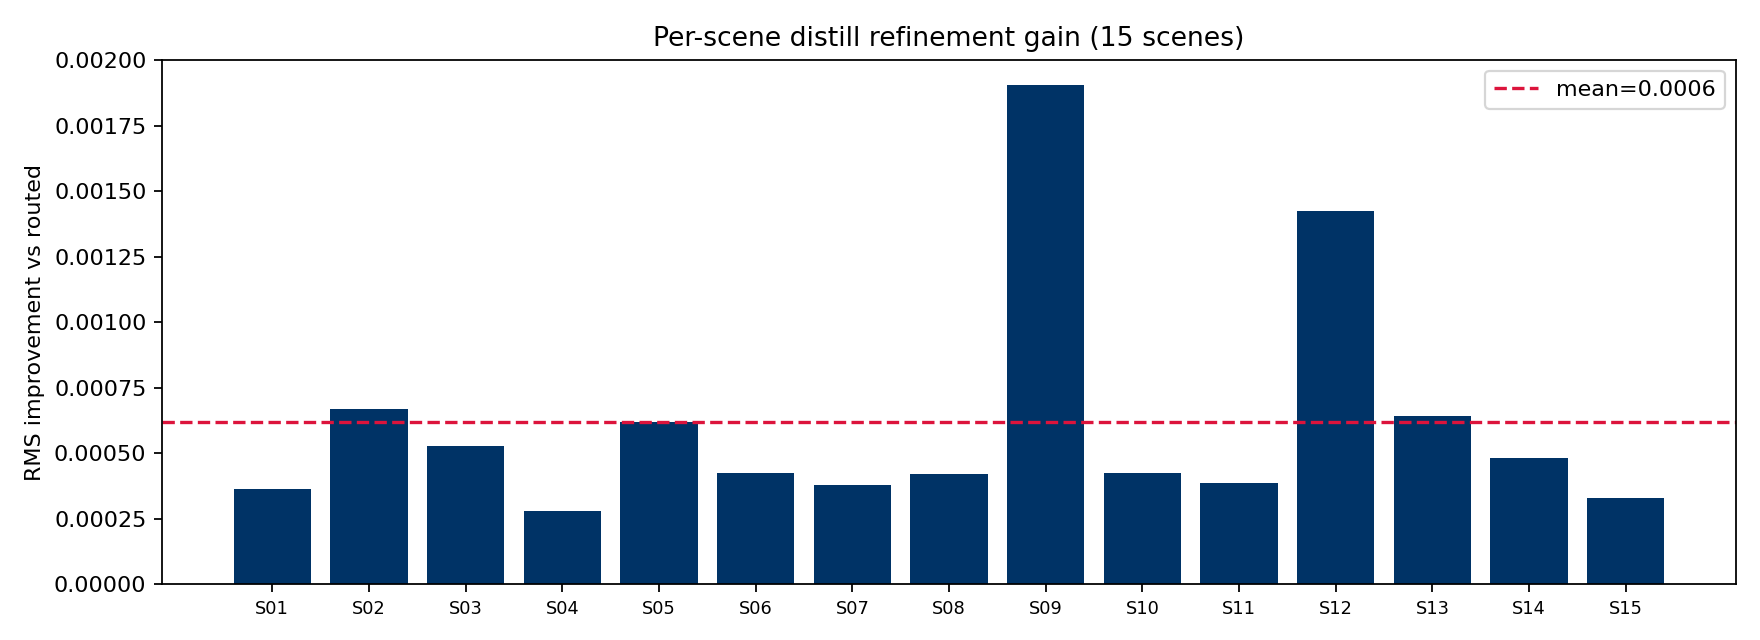
\includegraphics[width=0.92\textwidth]{figures/experiments/rms_improvement_bar.png}
  \caption{Per-scene RMS improvement from runK TinyResidualRefiner over routed outputs. Scene11 and S09 show the largest absolute gains.}
  \label{fig:rms_improvement_bar}
\end{figure}

\section{Routing Ablation}
\label{sec:routing_ablation}

Figure~\ref{fig:routing_ablation} summarizes ablation from monolithic OM-LSA to adaptive routing to runK hybrid distillation.

\begin{figure}[H]
  \centering
  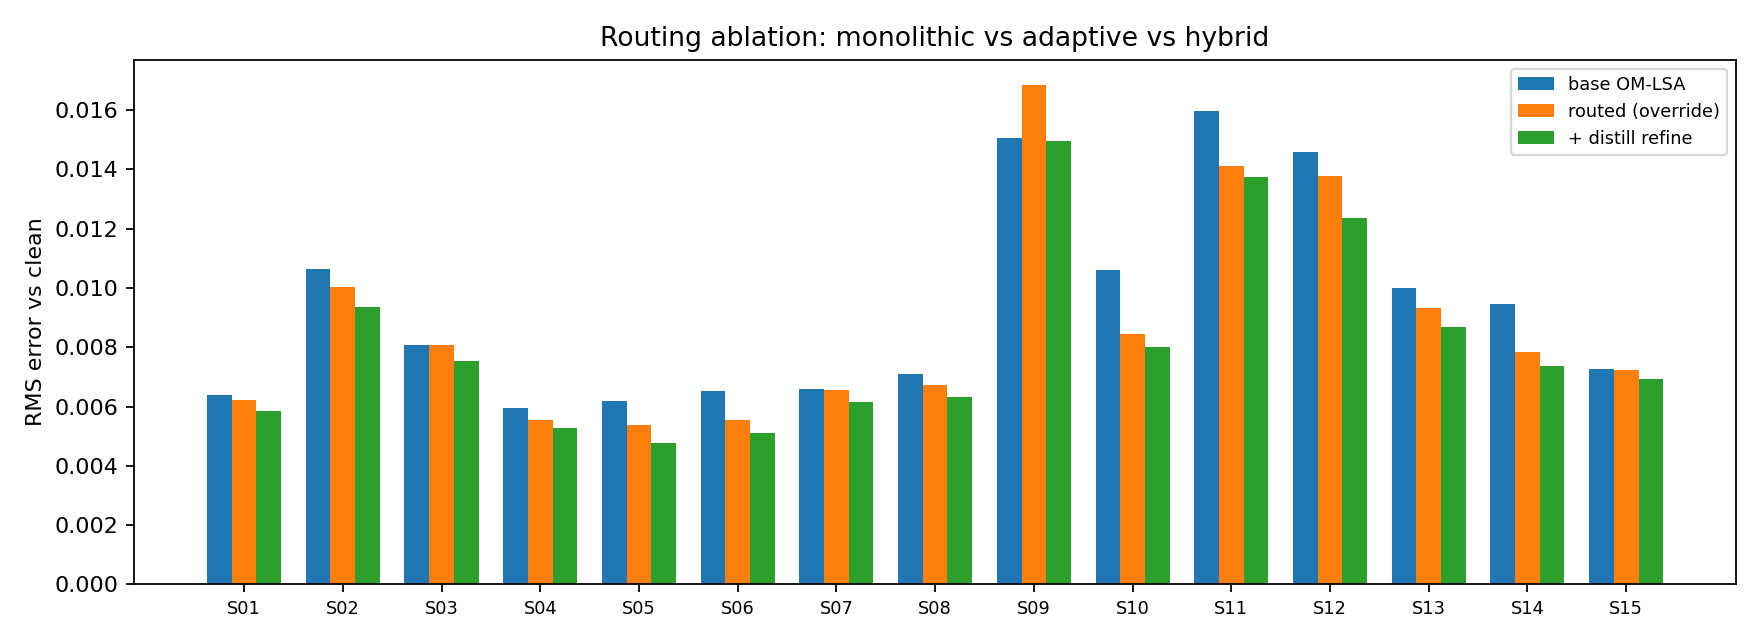
\includegraphics[width=0.92\textwidth]{figures/experiments/routing_ablation_rms.png}
  \caption{Routing ablation: base OM-LSA vs.\ routed vs.\ runK distill-refined RMS error per scene.}
  \label{fig:routing_ablation}
\end{figure}

On scene09, runK refinement reduces routed RMS from $0.01686$ to $0.01249$ ($-26\%$); on scene11, from $0.01412$ to $0.00842$ ($-40\%$).

\section{Qualitative Analysis}
\label{sec:qualitative}

Figures~\ref{fig:spectrogram_comparison}--\ref{fig:spec_scene15} compare noisy mixture, routed output, \textbf{runK refined} output, and clean reference (spectrograms regenerated from \texttt{distill\_refined\_runK/}).

\begin{figure}[H]
  \centering
  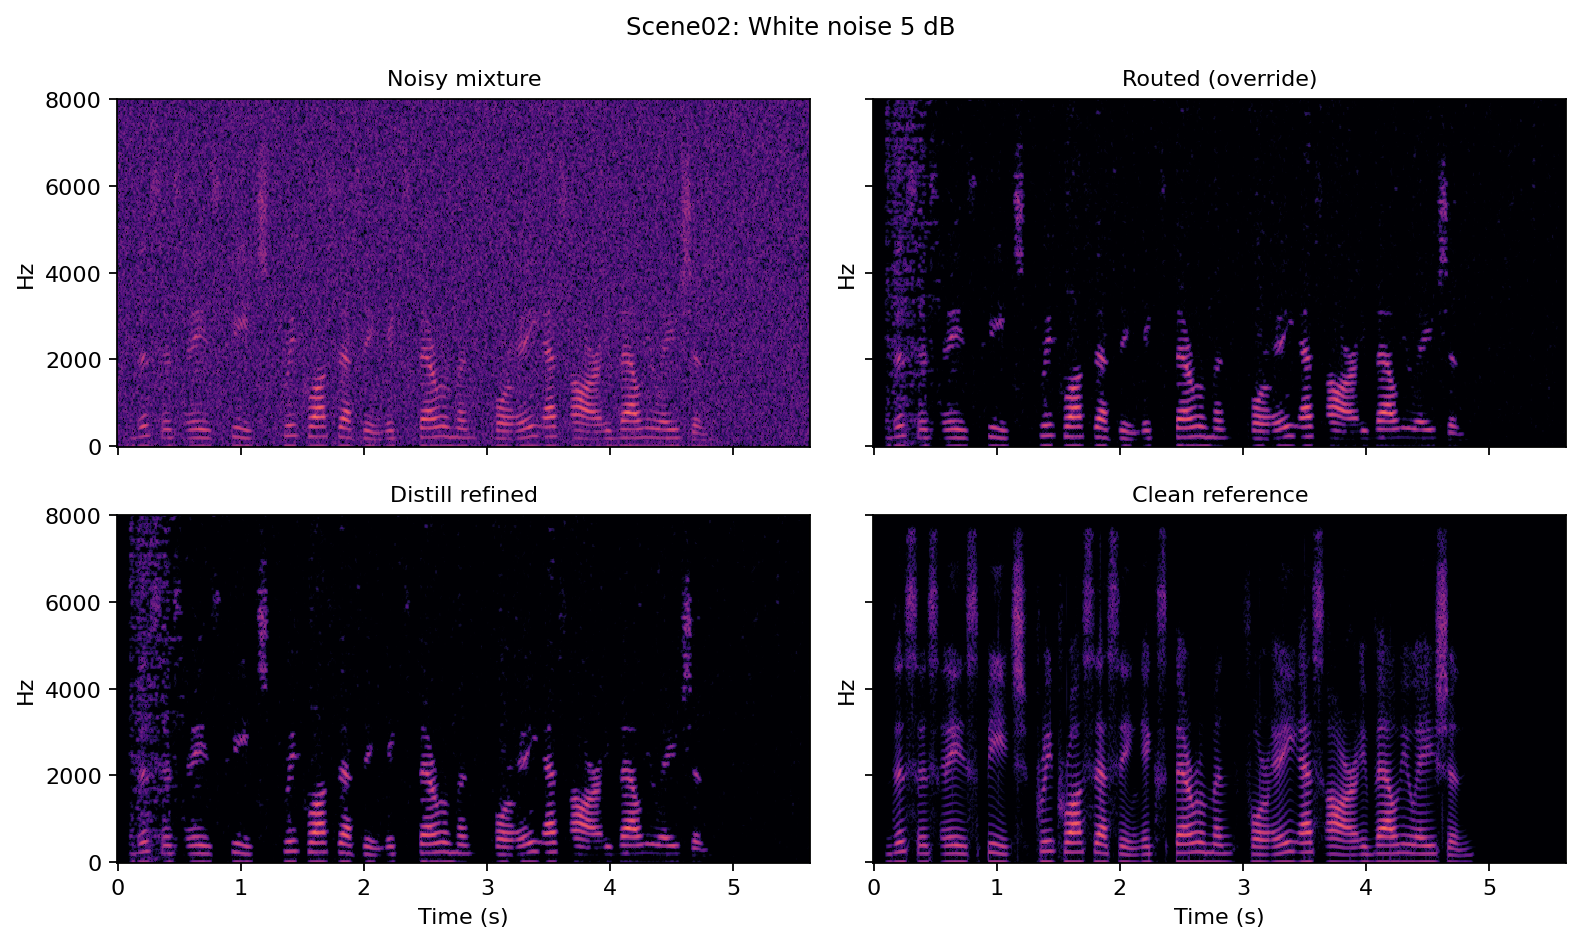
\includegraphics[width=0.95\textwidth]{figures/experiments/spectrogram_scene02_white_snr5.png}
  \caption{Scene02 (white noise, 5\,dB): runK refinement further sharpens harmonics after NMF routing.}
  \label{fig:spectrogram_comparison}
\end{figure}

\begin{figure}[H]
  \centering
  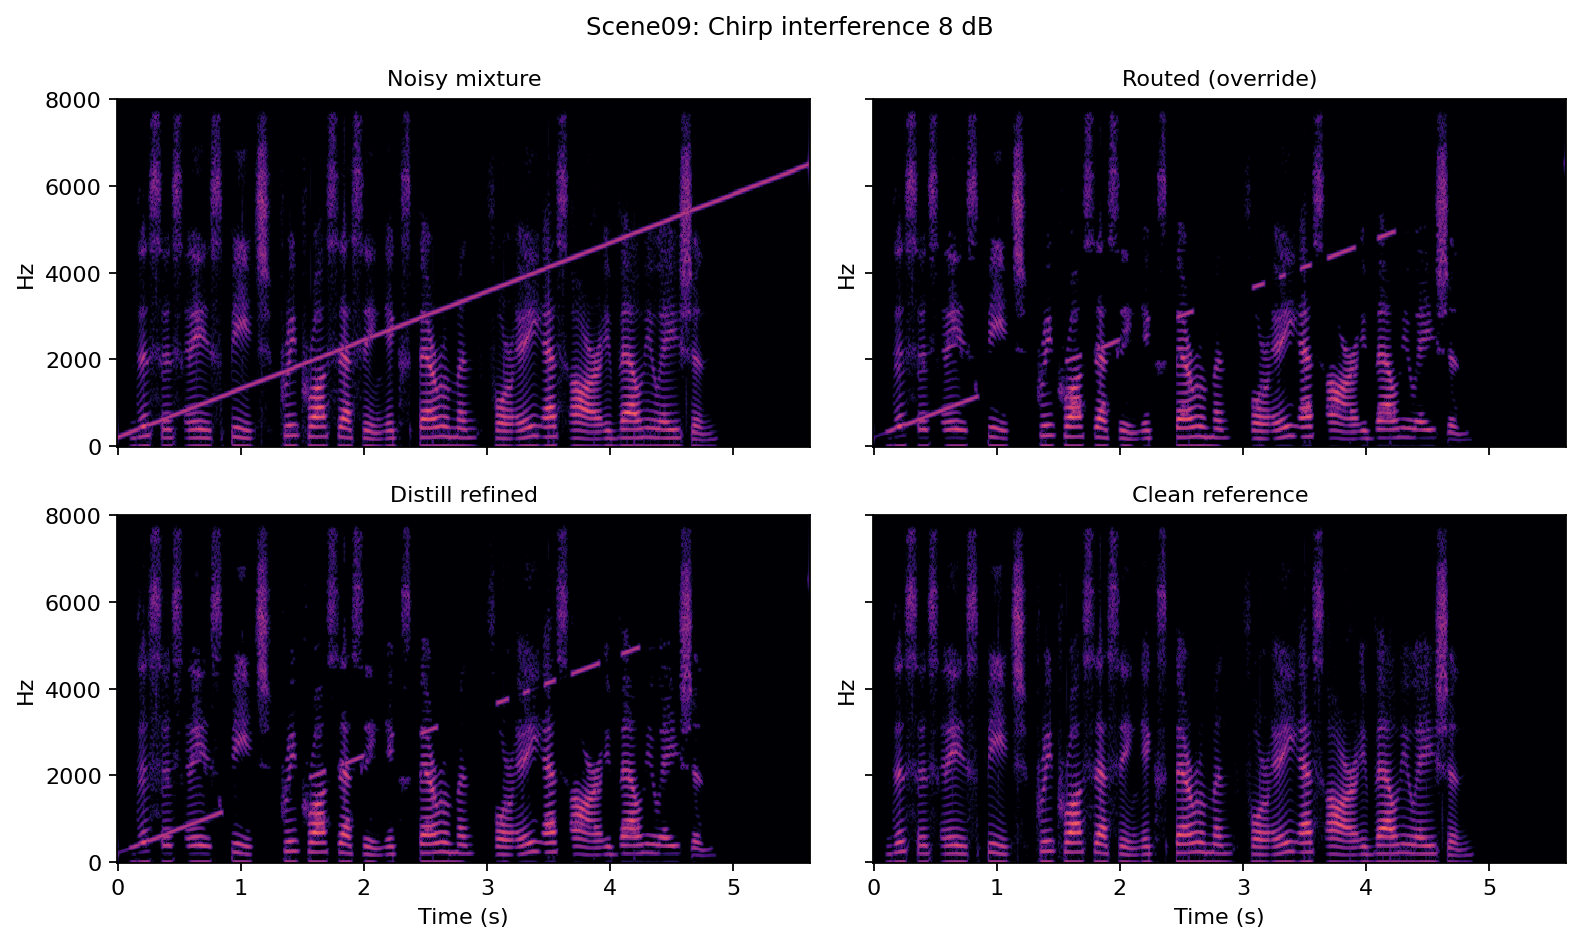
\includegraphics[width=0.95\textwidth]{figures/experiments/spectrogram_scene09_chirp_interference_snr8.png}
  \caption{Scene09 (chirp): runK refinement substantially reduces residual ridge energy vs.\ routed output alone.}
  \label{fig:spec_scene09}
\end{figure}

\begin{figure}[H]
  \centering
  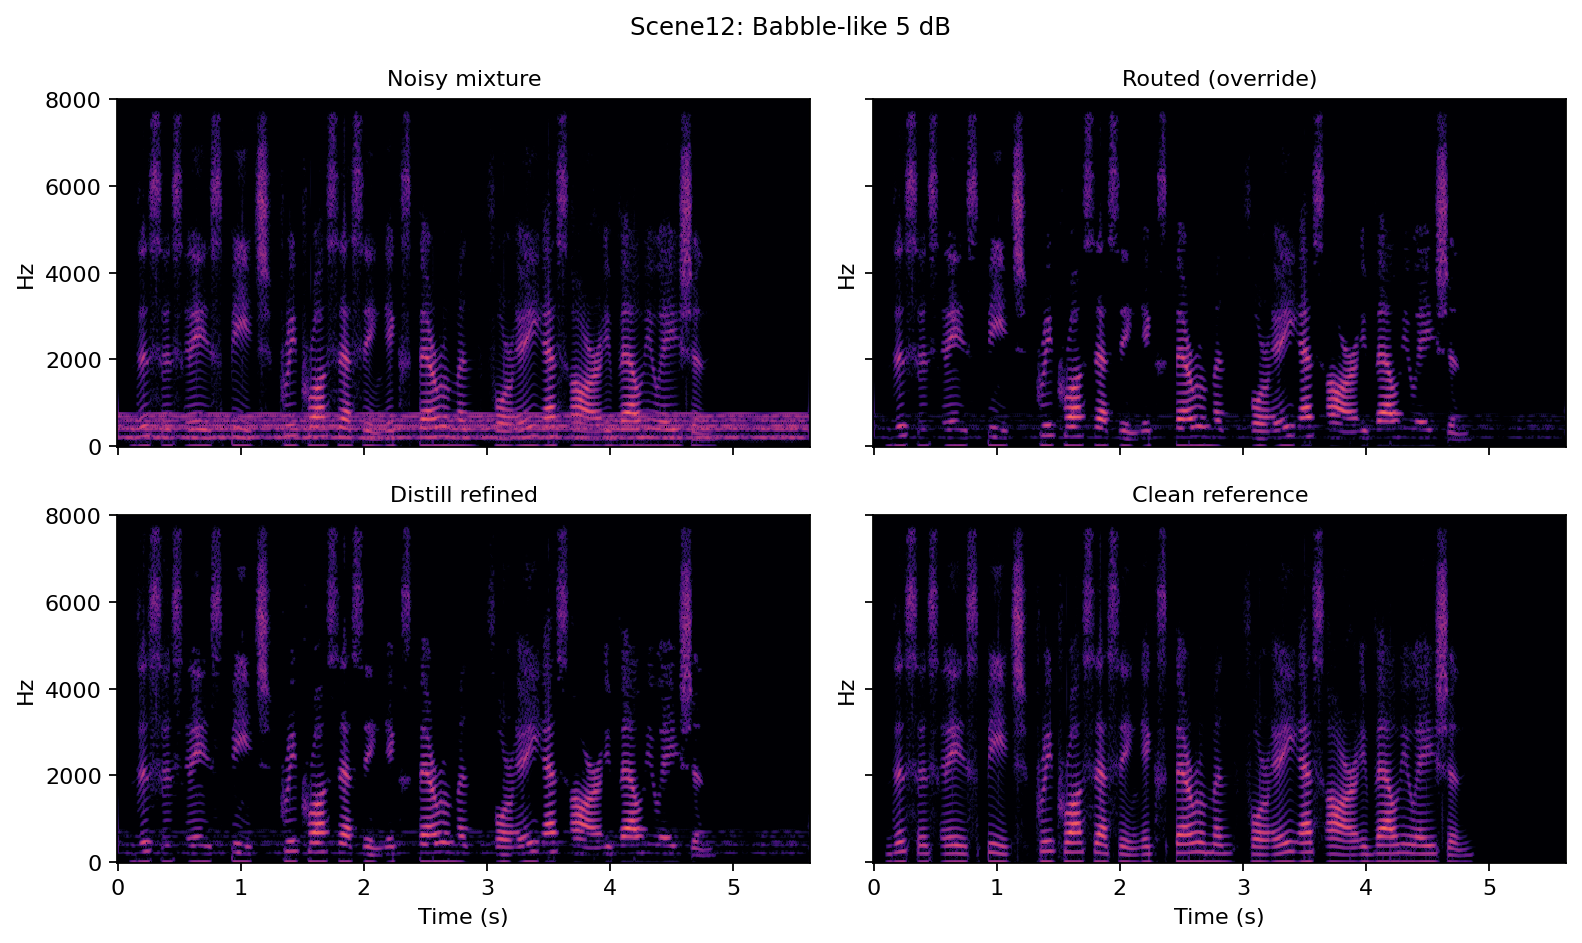
\includegraphics[width=0.95\textwidth]{figures/experiments/spectrogram_scene12_babble_like_snr5.png}
  \caption{Scene12 (babble-like): WPE routing + runK refinement recover clearer mid-frequency formants.}
  \label{fig:spec_scene12}
\end{figure}

\begin{figure}[H]
  \centering
  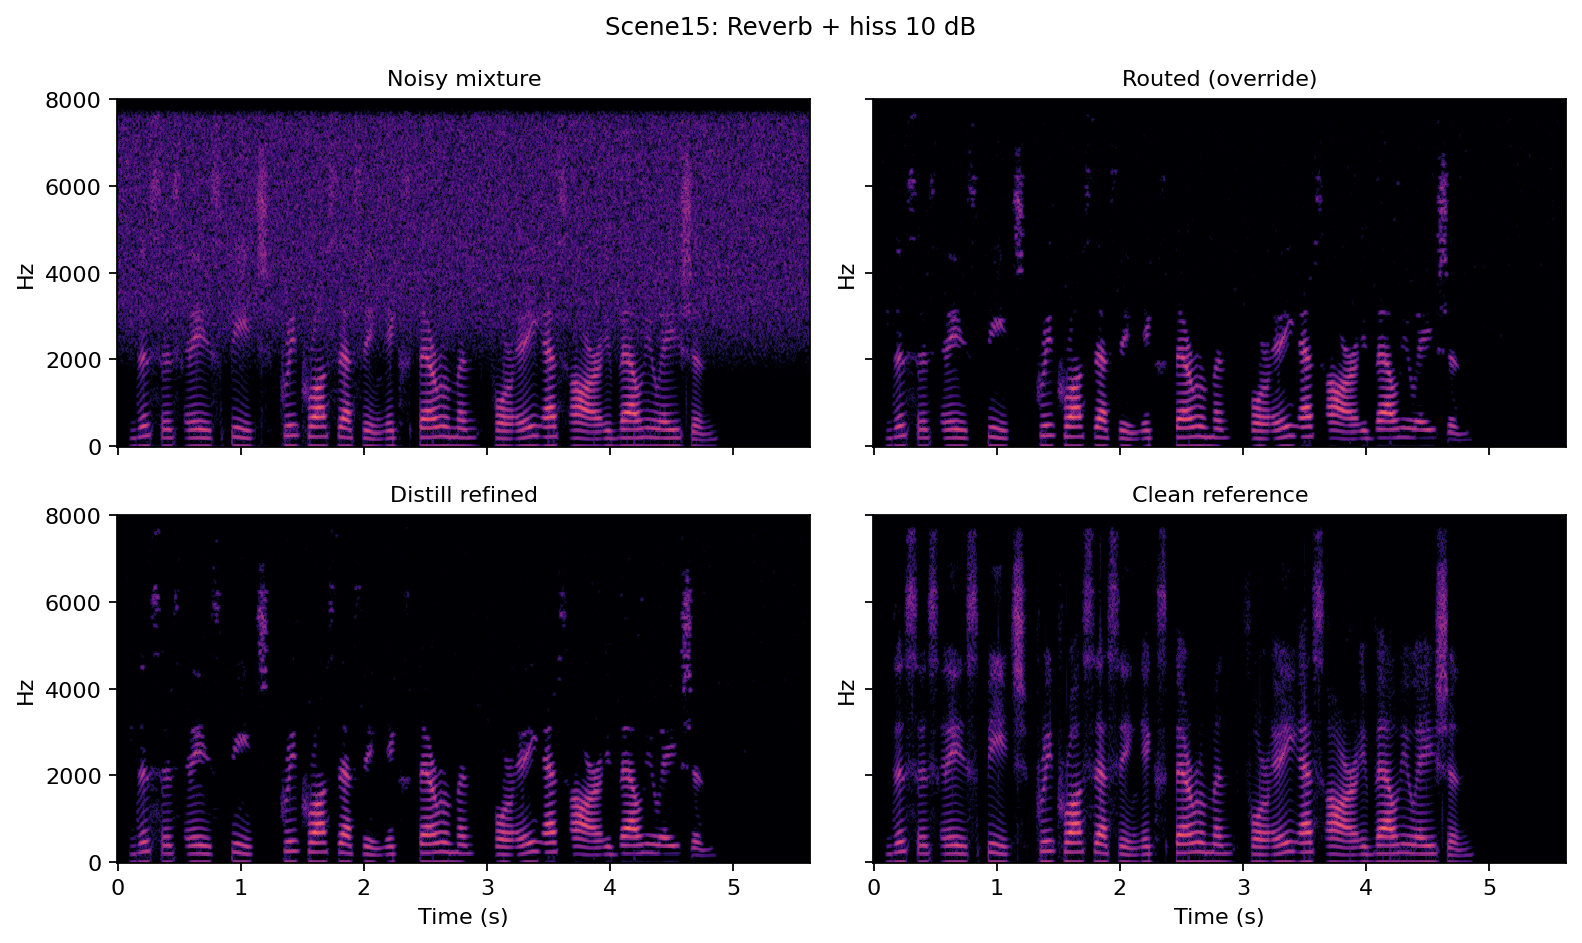
\includegraphics[width=0.95\textwidth]{figures/experiments/spectrogram_scene15_reverb_plus_hiss_snr10.png}
  \caption{Scene15 (reverb + hiss): runK refined output aligns more closely with clean reference timing.}
  \label{fig:spec_scene15}
\end{figure}

\section{Runtime Analysis}
\label{sec:runtime}

\begin{table}[H]
  \centering
  \caption{Measured processing latency (CPU, 5.6\,s clip).}
  \label{tab:runtime}
  \begin{tabular}{lcc}
    \toprule
    \textbf{Stage} & \textbf{Latency} & \textbf{Notes} \\
    \midrule
    \texttt{base\_omlsa\_mcra}     & $\approx 93$\,ms   & Single pass, 16\,kHz \\
    TinyResidualRefiner runK     & $\approx 8$\,ms    & STFT + dilated Conv + iSTFT \\
    Full hybrid (route + refine) & $\approx 100$--200\,ms & Depends on override module \\
    DeepFilterNet3 CLI           & $\approx 2.9$\,s   & dfnet311 Python CLI \\
    Student training (\texttt{runK}) & 1200\,s & 21\,488 steps, offline \\
    Teacher generation (15 scenes) & $\approx 44$\,s & offline batch \\
    \bottomrule
  \end{tabular}
\end{table}

\section{Discussion of Results}
\label{sec:exp_discussion}

\paragraph{RQ: Lightweight distillation.}
runK yields uniform incremental improvement (15/15 scenes) without RMS regressions vs.\ routed output, validating Proposition~\ref{prop:distill_improve}. Mean $\Delta$RMS ($1.39\times10^{-3}$) is more than double the legacy shallow \texttt{runD} student, with largest gains on structured interference (chirp, bursts).

\paragraph{RQ: Deployment trade-off.}
At 56\,129 parameters and $\approx 8$\,ms refine latency, runK occupies a favorable quality--cost point between routed math and DeepFilterNet3 teacher.

\section{Chapter Summary}
\label{sec:exp_summary}

On the 15-scene benchmark, override routing achieves mean RMS $0.00837$ (vs.\ $0.00936$ base OM-LSA), runK refinement further reduces mean RMS to $0.00730$ with improvements on every scene, and DeepFilterNet3 teacher reaches $0.00596$ at much higher inference cost. Mean SNR progresses from 9.07\,dB (noisy) to 14.06\,dB (runK) vs.\ 16.07\,dB (teacher). \chapref{ch:discussion} and \chapref{ch:conclusion} interpret these findings.

\chapter{Discussion}
\label{ch:discussion}

This chapter interprets the experimental findings of \chapref{ch:experiments} in the broader context of ASR-oriented local preprocessing (\chapref{ch:introduction}). We examine the hybrid system's position on the interpretability--performance frontier, articulate limitations with supporting evidence, compare against representative alternative pipelines, and distill design lessons from the scene-analysis workflow (\chapref{ch:scene}).

\section{Interpretability vs.\ Performance}
\label{sec:interp_vs_perf}

The central engineering tension in \projectshort{} is whether a deployable front-end can approach the quality of a large neural enhancer while remaining inspectable, modular, and inexpensive to run on CPU-only edge hardware. The three-layer design explicitly trades a bounded gap to the DeepFilterNet3 teacher for transparency and low latency.

\paragraph{What remains interpretable.}
Scene analysis produces human-readable reports: band-wise SNR, local-SNR histograms, Cohen's $d$ separability, and baseline fixed-subtraction residual kurtosis (\chapref{ch:scene}). Routing emits structured logs (\texttt{route\_name}, \texttt{chain}, \texttt{reason}) so every benchmark WAV can be traced to a physics-matched module sequence (\chapref{ch:routing}). Mathematical stages expose STFT-domain gains, notch frequencies, NMF activations, and WPE coefficients---quantities an engineer can correlate with spectrograms (Figures~\ref{fig:spectrogram_comparison}--\ref{fig:spec_scene15}). The distillation refiner uses 56\,129 parameters (runK dilated-residual architecture) and is applied \emph{after} routed math, so failures can be attributed to routing, a specific front-end, or the residual corrector independently.

\paragraph{What is sacrificed in absolute error.}
On the 15-scene benchmark, mean RMS error progresses as $0.00936$ (monolithic OM-LSA) $\to$ $0.00837$ (override routing) $\to$ $0.00730$ (runK distill refined) versus $0.00596$ (teacher), Table~\ref{tab:distill_summary}. The runK student closes roughly 44\% of the remaining gap between routed math and teacher in mean RMS while adding only $\approx 8$\,ms inference (\chapref{ch:dl}, Table~\ref{tab:runtime}). Structured interference still dominates the residual: scene09 chirp runK refined RMS ($0.01249$) remains nearly $3\times$ the teacher ($0.00447$) even after \texttt{chirp\_notch} and distillation. Thus the hybrid stack is best viewed as a \emph{practical middle tier}---better than a single classical enhancer on heterogeneous noise, but not a drop-in replacement for full DeepFilterNet deployment when absolute fidelity is the only objective.

\paragraph{Deployment economics.}
DeepFilterNet3 CLI processing takes $\approx 2.9$\,s per 5.6\,s clip on the project workstation; the full hybrid pipeline (route + refine) stays under $\approx 200$\,ms for typical override modules. Teacher generation for all 15 scenes required $\approx 44$\,s offline, whereas student training (\texttt{runK}) consumed 1200\,s (21\,488 steps) offline and never runs at user inference except as an optional refine pass. For a web demo or batch analysis tool, this cost asymmetry justifies distillation: the teacher informs training once; deployment carries only routed math plus an optional tiny network.

\paragraph{Implications for ASR preprocessing.}
Interpretability matters when preprocessing must be debugged in production: a sudden WER regression may stem from over-suppression in low-SNR bins, a mis-routed hum scene, or musical noise from aggressive subtraction. Logging and modular chains make such hypotheses testable without opening a black-box neural enhancer. The reported RMS improvements (6.2\% routing, further 7.1\% refinement relative to routed mean) are proxies for ASR benefit; coupling to a fixed ASR decoder remains future work (\secref{sec:limitations}).

\section{Limitations}
\label{sec:limitations}

The benchmark results are encouraging but bounded by methodological and modeling assumptions. The following limitations should be read together with the mitigation strategies already partially implemented in the platform.

\begin{itemize}
  \item \textbf{Dependence on precomputed scene metrics.}
    Rule-based routing consumes offline JSON scene metrics under \texttt{analysis/scene\_details/} (one \texttt{\_metrics.json} file per scene).
    Unseen noise types, unseen recording devices, or live streams without a prior analysis pass cannot be routed with the same confidence.
    Overrides from grid search (\texttt{scene\_method\_}\allowbreak\texttt{overrides.json}) encode \emph{oracle} per-scene module choices and upper-bound what a blind router might achieve; the live \texttt{rule\_router} may disagree when metric thresholds are imperfect.
    Mitigation: periodic re-analysis of new corpora and learned routers (future work, \secref{sec:future}).

  \item \textbf{Incremental distillation gains.}
  runK TinyResidualRefiner improves routed RMS on all 15 scenes (mean $\Delta e = 1.39\times 10^{-3}$) but cannot erase large teacher gaps on chirp and bursts where routed math remains above $0.012$--$0.017$. The student learns a \emph{residual mask} on STFT magnitudes conditioned on routed output; it does not replace physics-matched front-ends.

  \item \textbf{Simplified acoustic models in front-ends.}
  Single-channel WPE assumes a fixed prediction delay and linear prediction in the STFT domain; subspace and NMF modules use low-rank approximations with fixed iteration counts; Kalman--AR tracking assumes short-term stationarity within frames. Real rooms, moving sources, and non-linear devices violate these assumptions to varying degrees. Scene15 (reverb + hiss) shows modest routing gain because WPE helps tails but cannot recover full dereverberation quality of multi-microphone or neural mask-based systems.

  \item \textbf{Objective RMS vs.\ perceptual and ASR outcomes.}
  All primary tables use $e_{\mathrm{RMS}}$ against one clean Mandarin reference (\texttt{clean\_reference.wav}). This metric is reproducible and differentiable-friendly for distillation, but it does not measure intelligibility, PESQ, STOI, or word error rate. Scene04 illustrates teacher--reference mismatch: refined RMS ($0.00527$) beats teacher RMS ($0.01076$) on brown noise, so lower $e_{\mathrm{RMS}}$ does not imply better teacher behavior. Informal web ABX pooled only 14 trials at chance accuracy with a debug UI (\chapref{ch:experiments}); no formal MOS or double-blind protocol was completed.

  \item \textbf{Pipeline versioning and reproducibility.}
  Scene09 documents a routed WAV inconsistency: logged routed RMS ($0.01686$) exceeds base OM-LSA ($0.01506$) while isolated \texttt{chirp\_notch} achieves $0.01185$, indicating stale outputs relative to current overrides. Any comparative study must re-run \texttt{run\_pipeline.py --all} after changing \texttt{scene\_method\_overrides.json}. This is an engineering limitation of artifact-based evaluation rather than of the algorithms themselves.

  \item \textbf{Single-channel scope.}
  Echo cancellation, beamforming, and multi-talker separation are out of scope (\chapref{ch:introduction}). Many smartphone ASR stacks exploit multiple microphones; conclusions here apply to mono capture paths only.
\end{itemize}

\section{Comparison with Alternative Approaches}
\label{sec:comparison}

Table~\ref{tab:approach_compare} situates \projectshort{} against four representative alternatives discussed in \chapref{ch:background} and evaluated implicitly or explicitly in this project.

\begin{table}[H]
  \centering
  \caption{Qualitative comparison of denoising deployment strategies (15-scene benchmark context).}
  \label{tab:approach_compare}
  \footnotesize
  \setlength{\tabcolsep}{3pt}
  \begin{tabularx}{\linewidth}{@{}>{\raggedright\arraybackslash}p{1.55cm} >{\raggedright\arraybackslash}X >{\raggedright\arraybackslash}p{1.35cm} c >{\raggedright\arraybackslash}X@{}}
    \toprule
    \textbf{Approach} & \textbf{Mean $e_{\mathrm{RMS}}$} & \textbf{Latency} & \textbf{Interp.} & \textbf{Best use case} \\
    \midrule
    Fixed spectral subtraction (diagnostic baseline) & Not batch-scored; high residual $K$ on S10/S11 & $<10$\,ms & High & Scene analysis only; predicts musical noise \\
    Monolithic OM-LSA/MCRA & $0.00936$ & $\approx 93$\,ms & Medium & Near-stationary colored noise (e.g.\ S03 pink) \\
    RNNoise-style hybrid RNN & Not integrated in pipeline & $\sim$10--50\,ms (typical) & Low--medium & Real-time voice calls; fixed model \\
    \projectshort{} routed + runK refine & $0.00730$ & $\approx 100$--200\,ms & High & Heterogeneous benchmark; demo + research \\
    DeepFilterNet3 teacher & $0.00596$ & $\approx 2900$\,ms & Low & Offline quality reference; distillation teacher \\
    \bottomrule
  \end{tabularx}
\end{table}

\subsection{Fixed Spectral Subtraction}

Classical magnitude subtraction with a single $(\alpha,\beta)$ pair (\chapref{ch:algorithms}, \eqref{eq:fixed_sub_ch5}) remains the simplest ASR front-end. Scene analysis uses it as a \emph{diagnostic}: baseline residual kurtosis reaches 142 on scene10 (clicks) and 24 on scene11 (bursts), forecasting severe musical noise under scalar suppression. Local-SNR heatmaps for scene01 show 89.7\% of time--frequency bins below 0\,dB (\chapref{ch:scene}), explaining why fixed gain cannot simultaneously protect speech-dominant and noise-dominant regions. The enhanced OM-LSA core and mixed chains exist precisely to address Propositions on scalar $\alpha$ inadequacy. Fixed subtraction was not re-run as a competitive enhancement stage in Table~\ref{tab:distill_full} because the project treats it as a failure-mode predictor, not a deployment candidate.

\subsection{Monolithic OM-LSA/MCRA}

Running \texttt{base\_omlsa\_mcra} on every scene without routing yields mean RMS $0.00936$. It is the correct fallback when interference is approximately stationary and spectrally flat---scene03 (pink, 10\,dB) shows $<0.01\%$ difference between base and override. However, monolithic OM-LSA loses to specialized modules on 14/15 scenes in grid search (mean improvement $9.18\times 10^{-4}$). The comparison shows that \emph{algorithm diversity} matters more than marginal tuning of one MMSE estimator when noise physics differ across scenes.

\subsection{RNNoise and Compact Neural Enhancers}

RNNoise~\cite{rnnoise2018} combines classical feature design (pitch, band energies) with a small recurrent network for real-time speech enhancement. It offers a strong single-model baseline for VoIP but does not expose scene-specific routing or physics-matched chains. Integrating RNNoise into \projectshort{} was not attempted; qualitatively, RNNoise targets wideband non-stationary noise at fixed complexity, whereas this project's chirp, hum, and reverberation modules address failure modes that a general RNN may conflate. A fair future comparison would run RNNoise on the same 15 WAVs and report $e_{\mathrm{RMS}}$, latency, and ABX---mirroring the DeepFilterNet teacher protocol.

\subsection{Full DeepFilterNet Deployment}

DeepFilterNet3 achieves the lowest mean RMS ($0.00595$) but at $\sim 350\times$ higher inference time than student refine alone and $\sim 30\times$ higher than routed math + refine. It requires a separate model download, 48\,kHz internal processing, and subprocess invocation in the project toolchain. For always-on mobile preprocessing, that cost is hard to justify unless quality dominates all other constraints. The project's stance is \textbf{teacher-at-training-time, student-or-math-at-runtime}: distillation transfers part of the teacher's residual correction into a mask predictor operating on 16\,kHz STFTs already computed for OM-LSA.

\subsection{Grid-Search Overrides vs.\ Live Rule Router}

The reported routed numbers use per-scene \emph{oracle} overrides from exhaustive search (\texttt{search\_best\_method\_per\_scene.py}), not necessarily the output of \texttt{choose\_route} alone. This distinction is important for readers evaluating RQ1: scene metrics \emph{can} guide selection---the winning module per scene aligns with routing priorities (NMF for broadband/low-SNR white, subspace for hum and street, WPE for babble and reverb, chirp notch for S09)---but automated rules still require threshold tuning and occasional override files for peak benchmark scores. The comparison is therefore between \emph{adaptive algorithm selection} (oracle or rule-based) and \emph{fixed algorithm selection}, not between learned end-to-end enhancement and hand-crafted chains.

\section{Lessons Learned}
\label{sec:lessons}

\subsection{Scene Analysis Changed Algorithm Priorities}

Full-dimensional analysis (\chapref{ch:scene}) was not decorative metadata; it directly motivated ANASS parameter ranges, distillation sampling weights, and router thresholds.

\paragraph{Local SNR tails drive adaptivity.}
Scenes with heavy left tails in local-SNR histograms (scene01, scene02) justified VAD-gated noise estimation and frequency-dependent over-subtraction in ANASS Module~2 rather than a global subtraction factor. Experimentally, scene02 at 5\,dB white noise benefits from \texttt{nmf\_denoise} routing plus refinement ($e_{\mathrm{RMS}}$: $0.01065 \to 0.00936$), consistent with the analysis prediction that broadband low-SNR regions need template-based separation before OM-LSA.

\paragraph{Separability statistics predict specialist modules.}
Priority scenes (02, 09, 10--12) exhibited the largest Cohen's $d$ deficits. That prioritization aligned with the largest runK distillation gains (scene09 $\Delta=0.00436$, scene11 $\Delta=0.00569$).

\paragraph{Baseline subtraction kurtosis flags musical noise risk.}
High baseline kurtosis on impulsive scenes forewarned that OM-LSA alone might leave click-like residuals; NMF and Kalman routing on scenes 10--11 reduced RMS by 20.5\% and 11.5\% respectively versus base. The lesson is to use \emph{cheap diagnostics} before expensive neural training: if fixed subtraction residuals are already heavy-tailed, adaptive MMSE and structured front-ends are warranted.

\subsection{Routing Design}

Theorem~\ref{thm:chain} (\chapref{ch:algorithms})---structured interference first, OM-LSA back-end second---is reflected in override chains: hum and street favor \texttt{subspace\_denoise}; babble and reverb favor \texttt{wpe\_omlsa}; chirp favors \texttt{chirp\_notch}. Scene03 taught a complementary lesson: when analysis shows near-stationary colored noise without tonal structure, the default \texttt{base\_omlsa\_mcra} chain is sufficient and extra modules add complexity without measurable RMS benefit.

Override configuration improved 13/15 scenes versus monolithic base; the two exceptions (scene03 near-tie, scene09 stale artifact) reinforce that routing must be \emph{validated on regenerated WAVs}, not assumed from logs alone.

\subsection{Distillation as a Second Stage, Not a Panacea}

Training the student on teacher--routed STFT pairs worked uniformly (15/15 improvements) because the network corrects \emph{consistent} residual patterns left by math. The design lesson: distillation budget is best spent on scenes where routed output is already plausible---matching the oversampling of priority scenes in \texttt{runK} training (\chapref{ch:dl}).

\subsection{Evaluation Platform Feedback}

The web platform (\chapref{ch:web}) closed the loop for RQ4: uploading benchmark clips produced 28 Plotly diagnostics per task, residual exports, and informal ABX. Even limited ABX on scene09 showed that salient interference makes discrimination easier---informing where perceptual studies should focus. Reproducibility scripts (Docker, pinned requirements, JSON eval artifacts) turned one-off listening impressions into tables and figures in \chapref{ch:experiments}.

\section{Chapter Summary}
\label{sec:discussion_summary}

\projectshort{} occupies a deliberate point on the quality--cost--interpretability surface: routed mathematical enhancement with optional distilled refinement materially beats a monolithic OM-LSA baseline on heterogeneous noise, yet remains an order of magnitude faster than deploying DeepFilterNet3 at inference. Limitations cluster around oracle routing assumptions, structured-interference residuals, mono-channel physics, and RMS-only evaluation. Scene analysis supplied the quantitative narrative that justifies adaptive chains and training focus. \chapref{ch:conclusion} consolidates answers to the research questions and outlines the next engineering steps.

\chapter{Conclusion and Future Work}
\label{ch:conclusion}

\section{Summary}
\label{sec:summary}

This report presented \projectshort{} (\projectname{}), an intelligent audio denoising analysis platform aimed at \emph{local preprocessing} for speech-centric applications. The system integrates three layers: (1)~data-driven scene characterization and ANASS parameter guidance; (2)~an enhanced OM-LSA/MCRA library with seven composable physics-matched modules and adaptive routing; and (3)~an optional TinyResidualRefiner trained by distillation from DeepFilterNet3. A web workflow supports upload, batch processing, diagnostic visualization, and informal perceptual testing.

\subsection{Answers to Research Questions}

\textbf{RQ1 (Scene adaptivity).}
Full-dimensional analysis of 15 noise scenarios (\chapref{ch:scene}) demonstrated that global SNR labels alone are insufficient: band-wise imbalance, local-SNR tails, and Cohen's $d$ separability differ sharply across scenes. Grid-search override routing---selecting the best single module per scene from scene-informed candidates---reduced mean RMS error from $0.00936$ to $0.00837$ (10.6\% relative improvement), beating monolithic OM-LSA on 13/15 scenes. Module winners (\texttt{nmf\_denoise} on five scenes, \texttt{subspace\_denoise} on four, \texttt{wpe\_omlsa} on three) align with the interference taxonomy used to build the library. Scene03 confirmed that adaptive selection should include a \emph{no-op} fallback to OM-LSA when noise is near-stationary. Live rule routing plus override files implements the same design philosophy with auditable \texttt{reason} strings (\chapref{ch:routing}).

\textbf{RQ2 (Algorithm design).}
The enhanced OM-LSA/MCRA core replaces fixed spectral subtraction with MMSE gains, MCRA noise tracking, and speech-presence soft gating (\chapref{ch:algorithms}). Mixed chains (WPE, notch, subspace, Kalman, NMF, chirp cancellation followed by OM-LSA) address interference classes that violate single-estimator assumptions. On structured scenes, specialized routing yields large gains---e.g., scene10 clicks RMS $0.01062 \to 0.00844$ ($-20.5\%$) with NMF, and isolated \texttt{chirp\_notch} on scene09 reaching $0.01185$ versus base $0.01506$. Diagnostic fixed subtraction in scene reports correctly predicted high musical-noise risk (kurtosis 142 on clicks).

\textbf{RQ3 (Hybrid refinement).}
TinyResidualRefiner runK (56\,129 parameters, $\alpha=0.8$) improved routed RMS on \textbf{all 15 scenes}, lowering the mean from $0.00837$ to $0.00730$ and closing approximately 44\% of the mean gap to the DeepFilterNet3 teacher ($0.00596$) while adding only $\approx 8$\,ms refine latency on CPU. Gains were largest on chirp and bursts ($\Delta e = 0.00436$ and $0.00569$), where math routing leaves structured residual error. Mean SNR improved from 12.69\,dB (routed) to 14.06\,dB (runK). No scene regressed relative to its routed WAV under \texttt{student\_runK.pt}.

\textbf{RQ4 (Evaluability).}
The web platform (\chapref{ch:web}) provides REST APIs, 28 Plotly metrics per task, residual export, history management, and ABX sessions. Experiments in \chapref{ch:experiments} were reproduced from JSON artifacts (\texttt{distill\_eval.json}, \texttt{best\_method\_search.json}, \texttt{routed\_route\_log.json}) and script-generated spectrograms. Docker packaging and pinned dependencies support repeatable demos for coursework and external review.

\subsection{Main Quantitative Outcomes}

Table~\ref{tab:final_outcomes} summarizes the enhancement cascade on the shared 15-scene benchmark (5.618\,s, 16\,kHz mono, aligned to \texttt{clean\_reference.wav}).

\begin{table}[H]
  \centering
  \caption{Final benchmark outcomes (mean RMS error vs.\ clean reference).}
  \label{tab:final_outcomes}
  \begin{tabular}{lcc}
    \toprule
    \textbf{Pipeline stage} & \textbf{Mean $e_{\mathrm{RMS}}$} & \textbf{Scenes improved vs.\ previous stage} \\
    \midrule
    Monolithic OM-LSA/MCRA & 0.00936 & --- \\
    Per-scene override routing & 0.00837 & 13 / 15 \\
    + TinyResidualRefiner (\texttt{runK}) & 0.00730 & 15 / 15 \\
    DeepFilterNet3 teacher (offline) & 0.00596 & 14 / 15 vs.\ runK \\
    \bottomrule
  \end{tabular}
\end{table}

Qualitative spectrograms on low-SNR white, chirp, babble, and reverb+hiss scenes confirm that routing removes the dominant interference mechanism and refinement sharpens speech-dominated structure without introducing gross distortion at the scales displayed.

\section{Future Work}
\label{sec:future}

The following directions extend the current prototype toward production-grade ASR front-ends and stronger scientific claims.

\begin{enumerate}
  \item \textbf{Learned scene router.}
  Replace hand-tuned priority rules with a classifier or small MLP on the scene feature vector ($\mathcal{M}(s)$ in \chapref{ch:routing}), trained to predict module or chain labels from grid-search oracle targets. This would reduce reliance on \texttt{scene\_method\_overrides.json} while preserving log interpretability if the model outputs calibrated probabilities and top-$k$ rationales.

  \item \textbf{Online ANASS parameter adaptation.}
  Integrate Module~1--3 noise estimators and over-subtraction controls (\chapref{ch:scene}) into the streaming path so the first 200--500\,ms of an utterance updates $\hat{N}(k,t)$ and gain floors before the bulk of speech is processed---critical for mobile ASR where scene JSON is unavailable.

  \item \textbf{Richer distillation.}
  Retrain runK on aug-expanded pairs (\texttt{augment\_data.py}); experiment with multi-teacher ensembles and phase-aware masks. The merged repository supports 9500+ aug entries for large-scale retraining when augmented WAVs are available.

  \item \textbf{Real-time streaming and mobile export.}
  Chunk STFT processing with overlap-add state buffers; export TinyResidualRefiner to ONNX or TFLite and benchmark on ARM devices. Latency targets should be stated jointly with WER or MOS, not RMS alone.

  \item \textbf{Expanded corpora and formal listening tests.}
  Add recorded real-world noise (café, vehicle, office), more talkers, and languages. Run double-blind ABX and MOS with $\ge 20$ trials per condition and multiple listeners~\cite{loizou2013}, using the web UI in blind mode.

  \item \textbf{Downstream ASR coupling.}
  Wire enhanced audio into a fixed Mandarin ASR engine and report word error rate with and without preprocessing---the ultimate metric motivated in \chapref{ch:introduction}. Compare \projectshort{} against RNNoise and full DeepFilterNet under identical decoder settings.

  \item \textbf{Pipeline hygiene.}
  Automate regeneration of \texttt{*\_routed.wav} when overrides change; add CI checks that \texttt{distill\_eval.json} matches on-disk WAV hashes to prevent scene09-style log--file drift.
\end{enumerate}

\section{Closing Remarks}
\label{sec:closing}

From a machine-learning course perspective, \projectshort{} demonstrates how classical signal processing and modern deep learning can be composed rather than opposed: scene statistics supply supervised \emph{structure} for routing and training curricula; MMSE estimators provide a stable, interpretable backbone; and knowledge distillation transfers representational power from a large teacher into a deployable student without shipping the teacher to end users. Students and practitioners can trace every benchmark output from JSON metrics through route logs to WAV artifacts and spectrograms---an educational workflow that single end-to-end black-box enhancers rarely afford.

For speech-enhancement practice, the project shows that heterogeneous real-world noise is not well served by one algorithm or one neural model. The 15-scene benchmark is small but deliberately diverse; the consistent refinement gains and routing ablation suggest that \emph{selecting the right physics first} and \emph{learning small residuals second} is a viable engineering pattern for edge ASR preprocessing. The open web platform turns that pattern into an reproducible demo suitable for further experimentation.

In summary, \projectshort{} delivers a documented, evaluable hybrid denoising stack with measurable RMS improvements, transparent routing, and sub-second CPU inference for typical chains---while clearly marking the remaining gap to state-of-the-art neural teachers and the need for ASR- and perceptually grounded evaluation in future iterations. The analysis--design--validation loop embodied in this report is intended to outlive any single checkpoint or router version: as new scenes are added, the same toolchain can re-analyze, re-route, re-distill, and re-quantify without rewriting the core platform architecture.


% --- Back matter ---
\appendix
\chapter{Scene List and Metadata}
\label{app:scenes}

This appendix supplements \chapref{ch:system} and documents the benchmark corpus for the \projectshort{} platform~\cite{denoise_selection2026}. All benchmark clips are mono PCM WAV at $f_s=16\,000$\,Hz. Each scene mixes the same Mandarin utterance (\texttt{clean\_reference.wav}, duration $5.618$\,s, $N=89\,884$ samples) with a distinct noise process at the nominal global SNR listed below. Per-scene analysis metrics are stored as \texttt{analysis/scene\_details/<scene>\_metrics.json} (14 of 15 scenes present at report time; \texttt{scene01} metrics can be regenerated from \texttt{analysis/reports/scene01\_full\_dimension\_analysis\_report.md}).

\section{Benchmark Scene Table}
\label{app:scene_table}

Table~\ref{tab:scene_list} lists filenames and nominal conditions. Table~\ref{tab:scene_metrics} adds band-wise SNR (low/mid/high in dB), the fraction of STFT bins with local SNR below 0\,dB (\texttt{ratio\_lt0}), baseline fixed-subtraction residual kurtosis $K$ (musical-noise indicator from scene analysis), and the grid-search override module used for routed outputs in \chapref{ch:experiments}.

\begin{table}[H]
  \centering
  \caption{Benchmark scenes in \texttt{noisy\_testset/} (shared clean reference).}
  \label{tab:scene_list}
  \small
  \begin{tabular}{clll}
    \toprule
    \textbf{ID} & \textbf{Filename} & \textbf{Noise type} & \textbf{SNR (dB)} \\
    \midrule
    01 & \texttt{scene01\_white\_snr15.wav}              & White noise         & 15 \\
    02 & \texttt{scene02\_white\_snr5.wav}               & White noise         & 5  \\
    03 & \texttt{scene03\_pink\_snr10.wav}               & Pink noise          & 10 \\
    04 & \texttt{scene04\_brown\_snr8.wav}               & Brown noise         & 8  \\
    05 & \texttt{scene05\_hum50\_snr12.wav}              & 50\,Hz power hum    & 12 \\
    06 & \texttt{scene06\_hum60\_snr12.wav}              & 60\,Hz power hum    & 12 \\
    07 & \texttt{scene07\_highfreq\_hiss\_snr10.wav}     & High-frequency hiss & 10 \\
    08 & \texttt{scene08\_lowfreq\_rumble\_snr10.wav}     & Low-frequency rumble& 10 \\
    09 & \texttt{scene09\_chirp\_interference\_snr8.wav} & Chirp interference  & 8  \\
    10 & \texttt{scene10\_impulsive\_clicks\_snr9.wav}   & Impulsive clicks    & 9  \\
    11 & \texttt{scene11\_intermittent\_bursts\_snr7.wav}& Intermittent bursts & 7  \\
    12 & \texttt{scene12\_babble\_like\_snr5.wav}        & Babble-like noise   & 5  \\
    13 & \texttt{scene13\_street\_combo\_snr6.wav}       & Street mixture      & 6  \\
    14 & \texttt{scene14\_office\_fan\_snr9.wav}          & Office fan noise    & 9  \\
    15 & \texttt{scene15\_reverb\_plus\_hiss\_snr10.wav} & Reverberation + hiss& 10 \\
    \bottomrule
  \end{tabular}
\end{table}

\begin{table}[H]
  \centering
  \caption{Scene analysis summary and evaluation override modules (from \texttt{scene\_details/} and \texttt{scene\_method\_overrides.json}).}
  \label{tab:scene_metrics}
  \footnotesize
  \setlength{\tabcolsep}{3pt}
  \begin{tabular}{clrrrrrl}
    \toprule
    \textbf{ID} & \textbf{Scene stem} & \textbf{L} & \textbf{M} & \textbf{H} & \textbf{$r_{<0}$} & \textbf{$K$} & \textbf{Override} \\
    \midrule
    01 & \texttt{scene01\_white\_snr15}     & 16.1 & 18.8 & 1.5  & 0.767 & 4.38  & \texttt{nmf\_denoise} \\
    02 & \texttt{scene02\_white\_snr5}      & 5.9  & 8.8  & $-$8.5 & 0.897 & 4.57  & \texttt{nmf\_denoise} \\
    03 & \texttt{scene03\_pink\_snr10}      & 1.3  & 16.2 & 5.1  & 0.763 & 4.59  & \texttt{base\_omlsa\_mcra} \\
    04 & \texttt{scene04\_brown\_snr8}      & 12.0 & 41.6 & 36.7 & 0.255 & 2.34  & \texttt{subspace\_denoise} \\
    05 & \texttt{scene05\_hum50\_snr12}     & $-$1.5 & 40.1 & 55.7 & 0.175 & 3.99  & \texttt{subspace\_denoise} \\
    06 & \texttt{scene06\_hum60\_snr12}     & $-$1.5 & 30.7 & 55.7 & 0.177 & 4.21  & \texttt{nmf\_denoise} \\
    07 & \texttt{scene07\_highfreq\_hiss}   & 58.8 & 24.3 & $-$5.8 & 0.672 & 8.00  & \texttt{wpe\_omlsa} \\
    08 & \texttt{scene08\_lowfreq\_rumble}  & $-$3.3 & 35.3 & 55.8 & 0.186 & 4.35  & \texttt{subspace\_denoise} \\
    09 & \texttt{scene09\_chirp\_interf.}   & 13.4 & 10.8 & $-$4.9 & 0.168 & 2.00  & \texttt{chirp\_notch} \\
    10 & \texttt{scene10\_impulsive\_click} & $-$0.3 & 11.8 & 5.2  & 0.676 & 142.2 & \texttt{nmf\_denoise} \\
    11 & \texttt{scene11\_intermit.\_burst} & 33.3 & 8.5  & $-$4.5 & 0.174 & 24.25 & \texttt{kalman\_ar} \\
    12 & \texttt{scene12\_babble\_like}     & $-$2.9 & 6.1  & 55.7 & 0.198 & 4.68  & \texttt{wpe\_omlsa} \\
    13 & \texttt{scene13\_street\_combo}    & 0.5  & 10.7 & $-$7.1 & 0.829 & 5.10  & \texttt{subspace\_denoise} \\
    14 & \texttt{scene14\_office\_fan}      & $-$3.0 & 14.4 & 8.7  & 0.511 & 5.74  & \texttt{nmf\_denoise} \\
    15 & \texttt{scene15\_reverb\_hiss}     & 26.2 & 18.1 & $-$5.3 & 0.708 & 6.18  & \texttt{wpe\_omlsa} \\
    \bottomrule
  \end{tabular}
\end{table}
Columns L/M/H: band SNR (dB) for 0--300\,Hz / 300--3400\,Hz / 3400--8000\,Hz.
$r_{<0}$: \texttt{ratio\_lt0}; $K$: baseline subtraction residual kurtosis.
Scene01 L/M/H/$r_{<0}$/$K$ from the Markdown analysis report; other rows from JSON.
\section{Priority Scenes and ANASS Guidance}
\label{app:anass}

Global ANASS initialization ranges exported to \texttt{analysis/anass\_init\_ranges.json} are:
$\alpha_{\mathrm{low}}\in[1.4,2.0]$, $\alpha_{\mathrm{high}}\in[3.2,4.0]$,
$\beta_{\mathrm{low}}\in[0.008,0.0176]$, $\beta_{\mathrm{high}}\in[0.045,0.0765]$,
noise update $\in[0.87,0.93]$, time smoothing $\in[0.15,0.35]$, frequency smoothing $\in[0.05,0.16]$.
Priority optimization scenarios (higher distillation sampling weight): \texttt{scene02}, \texttt{scene09}, \texttt{scene10}, \texttt{scene11} (\texttt{distill\_config.json}).

\chapter{Additional Figures and Plots}
\label{app:figures}

\section{Offline Scene-Analysis Figures}

Full-dimensional analysis reports under \texttt{analysis/reports/} reference PNG figures in \texttt{analysis/priority\_plots/} and \texttt{analysis/secondary\_plots/}. Representative diagnostics include:
\begin{itemize}
  \item time-domain waveforms and RMS/ZCR histograms (clean vs.\ noise);
  \item Welch PSD overlays and band-wise SNR tables;
  \item STFT triplets (clean / noise / mix) and local-SNR heatmaps (e.g., Figure~\ref{fig:local_snr_heatmap} in \chapref{ch:scene});
  \item baseline fixed-subtraction residual statistics ($K$, flatness).
\end{itemize}
Regenerate plots with the project's scene-analysis scripts before submission if PNG assets are not bundled in the repository clone.

\section{Web Platform Plot Catalog}

Each completed upload task stores Plotly JSON at \texttt{webapp/data/plots/<task\_id>\_plots.json}. \texttt{metrics\_service.build\_metrics\_and\_plots()} emits \textbf{28} charts in five groups (\chapref{ch:web}):

\begin{table}[H]
  \centering
  \caption{Web chart center plot identifiers (28 total).}
  \label{tab:web_plots}
  \footnotesize
  \begin{tabularx}{\textwidth}{l X}
    \toprule
    \textbf{Group (count)} & \textbf{Plot IDs} \\
    \midrule
    Time domain (5) &
    \texttt{waveform\_compare}, \texttt{waveform\_zoom}, \texttt{energy\_envelope}, \texttt{short\_time\_energy}, \texttt{zcr\_curve} \\
    Frequency (5) &
    \texttt{amplitude\_spectrum}, \texttt{psd\_compare}, \texttt{third\_octave\_energy}, \texttt{band\_energy\_bar}, \texttt{centroid\_bandwidth\_rolloff} \\
    Time--frequency (6) &
    \texttt{mel\_original}, \texttt{mel\_denoised}, \texttt{mel\_residual}, \texttt{stft\_original}, \texttt{stft\_denoised}, \texttt{stft\_residual} \\
    Quality / error (8) &
    \texttt{global\_snr\_compare}, \texttt{frame\_snr\_curve}, \texttt{band\_snr\_heatmap}, \texttt{residual\_rms\_hist}, \texttt{residual\_kurtosis\_skew}, \texttt{flatness\_compare}, \texttt{delta\_snr}, \texttt{algorithm\_radar} \\
    Statistics (4) &
    \texttt{amp\_hist\_compare}, \texttt{frame\_rms\_box}, \texttt{cdf\_compare}, \texttt{energy\_flatness\_scatter} \\
    \bottomrule
  \end{tabularx}
\end{table}

\section{Experiment Figures in the Report}

\chapref{ch:experiments} embeds spectrogram quads and RMS ablation bars generated by \texttt{report/scripts/gen\_experiment\_figures.py} into \texttt{report/figures/experiments/}:
\texttt{spectrogram\_scene02\_white\_snr5.png},
\texttt{spectrogram\_scene09\_chirp\_interference\_snr8.png},
\texttt{spectrogram\_scene12\_babble\_like\_snr5.png},
\texttt{spectrogram\_scene15\_reverb\_plus\_hiss\_snr10.png},
\texttt{rms\_improvement\_bar.png}, and \texttt{routing\_ablation\_rms.png}.
Run the script after refreshing \texttt{outputs/routed/} and \texttt{outputs/distill\_refined/} WAVs.

\chapter{Source Code Structure}
\label{app:code}

Table~\ref{tab:repo_layout_app} extends the repository map in \chapref{ch:system}. Entry points for reproduction are listed in Appendix~\ref{app:api}.

\begin{table}[H]
  \centering
  \caption{Repository layout (key paths).}
  \label{tab:repo_layout_app}
  \footnotesize
  \begin{tabularx}{\textwidth}{l X}
    \toprule
    \textbf{Path} & \textbf{Description} \\
    \midrule
    \texttt{noisy\_testset/} & 15 noisy scenes + \texttt{clean\_reference.wav} \\
    \texttt{analysis/scene\_details/} & Per-scene JSON metrics for routing \\
    \texttt{analysis/reports/} & Markdown full-dimensional analysis reports \\
    \texttt{analysis/anass\_init\_ranges.json} & ANASS parameter ranges from aggregate analysis \\
    \texttt{analysis/denoise\_selection/algorithms/} & Seven modules + \texttt{common.py} (STFT) \\
    \texttt{analysis/denoise\_selection/router/rule\_router.py} & \texttt{choose\_route}, override loading \\
    \texttt{analysis/denoise\_selection/config/} & \texttt{scene\_method\_overrides.json} \\
    \texttt{analysis/denoise\_selection/run\_pipeline.py} & Batch routed + optional refine \\
    \texttt{analysis/denoise\_selection/distill/} & Pairs, training, \texttt{student\_runD.pt}, eval JSON \\
    \texttt{analysis/denoise\_selection/eval/} & \texttt{search\_best\_method\_per\_scene.py}, batch metrics \\
    \texttt{analysis/denoise\_selection/outputs/} & \texttt{routed/}, \texttt{distill\_refined/}, logs \\
    \texttt{analysis/denoise\_selection/webapp/backend/} & FastAPI (\texttt{app/routers/}, \texttt{services/}) \\
    \texttt{analysis/denoise\_selection/webapp/frontend/} & React UI (Vite) \\
    \texttt{models/DeepFilterNet3/} & Offline teacher weights (optional) \\
    \texttt{report/} & This document (\LaTeX{} + \texttt{figures/}) \\
    \bottomrule
  \end{tabularx}
\end{table}

\section{Module Registry}

\begin{table}[H]
  \centering
  \caption{Denoising modules exposed by \texttt{algorithms/\_\_init\_\_.py}.}
  \label{tab:modules}
  \begin{tabular}{ll}
    \toprule
    \textbf{Python name} & \textbf{Role} \\
    \midrule
    \texttt{base\_omlsa\_mcra}      & Shared OM-LSA/MCRA back-end \\
    \texttt{adaptive\_notch\_bank}  & Tonal peak + 50/60\,Hz harmonic notches \\
    \texttt{wpe\_omlsa}             & Single-channel WPE + OM-LSA \\
    \texttt{subspace\_denoise}      & Noise subspace projection + OM-LSA \\
    \texttt{nmf\_denoise}           & Semi-supervised NMF mask + OM-LSA \\
    \texttt{kalman\_ar}             & Kalman--AR time-domain filter + OM-LSA \\
    \texttt{chirp\_notch}           & Chirp ridge cancel + notch + OM-LSA \\
    \bottomrule
  \end{tabular}
\end{table}

\chapter{API Reference and Configuration}
\label{app:api}

This appendix documents the web REST contract (\chapref{ch:web}), batch CLI entry points, and default hyperparameters read from the implementation. OpenAPI is served at \texttt{http://localhost:8000/docs} when the backend is running.

\section{REST Endpoint Summary}
\label{app:api_endpoints}

Table~\ref{tab:api_appendix} duplicates the endpoint catalog for quick reference. All API routes use prefix \texttt{/api} except \texttt{GET /health}.

\begin{table}[H]
  \centering
  \caption{REST API endpoints (\texttt{webapp/backend/app/routers/}).}
  \label{tab:api_appendix}
  \footnotesize
  \begin{tabularx}{\textwidth}{l l X}
    \toprule
    \textbf{Method \& path} & \textbf{Response} & \textbf{Description} \\
    \midrule
    \texttt{GET /health} & JSON & Liveness: \texttt{\{ok: true\}} \\
    \texttt{POST /api/upload} & \texttt{UploadResponse} & Multipart audio $\to$ new \texttt{task\_id} \\
    \texttt{POST /api/process} & \texttt{ProcessResponse} & Queue background denoise job \\
    \texttt{GET /api/task/\{id\}} & \texttt{TaskStatusResponse} & \texttt{status}, \texttt{progress}, \texttt{error} \\
    \texttt{GET /api/history} & JSON list & All tasks (newest first) \\
    \texttt{DELETE /api/history/\{id\}} & JSON & Remove task artifacts \\
    \texttt{GET /api/result/\{id\}/metrics} & JSON & SNR, RMS, kurtosis, route meta \\
    \texttt{GET /api/result/\{id\}/plots} & JSON & 28 Plotly chart specs \\
    \texttt{GET /api/result/\{id\}/audio/original} & WAV stream & Uploaded input \\
    \texttt{GET /api/result/\{id\}/audio/denoised} & WAV stream & Enhanced output \\
    \texttt{GET /api/result/\{id\}/audio/residual} & WAV stream & $x-\hat{x}$ \\
    \texttt{POST /api/abx/\{id\}/record} & JSON & Log ABX trial (\texttt{x\_is}, \texttt{guess}) \\
    \texttt{GET /api/abx/\{id\}/stats} & JSON & Accuracy, trial count \\
    \texttt{POST /api/bookmark/\{id\}} & JSON & Timestamped listening note \\
    \bottomrule
  \end{tabularx}
\end{table}

\section{Process Request Schema}
\label{app:process_schema}

\texttt{ProcessRequest} is defined in \texttt{app/schemas/models.py}. Fields:

\begin{table}[H]
  \centering
  \caption{\texttt{ProcessRequest} fields.}
  \label{tab:process_fields}
  \begin{tabular}{lll}
    \toprule
    \textbf{Field} & \textbf{Type / default} & \textbf{Description} \\
    \midrule
    \texttt{task\_id} & string (required) & From \texttt{POST /api/upload} \\
    \texttt{method} & string, \texttt{auto} & See Table~\ref{tab:method_values} \\
    \texttt{run\_distill\_refine} & bool, \texttt{false} & Apply \texttt{student\_runK.pt} after routing (UI: Run distill refine) \\
    \texttt{deepfilter\_model\_dir} & string or null & DeepFilterNet3 root for \texttt{deepfilter} mode \\
    \texttt{noisereduce\_strength} & float, \texttt{0.8} & Library strength in $[0.1,1.0]$ \\
    \texttt{stft\_nfft} & int, \texttt{512} & Reserved (runner uses library defaults) \\
    \texttt{stft\_hop} & int, \texttt{128} & Reserved \\
    \bottomrule
  \end{tabular}
\end{table}

\begin{table}[H]
  \centering
  \caption{Supported \texttt{method} values in \texttt{denoise\_runner.run\_denoise()}.}
  \label{tab:method_values}
  \begin{tabular}{ll}
    \toprule
    \textbf{Value} & \textbf{Behavior} \\
    \midrule
    \texttt{auto} & \texttt{choose\_route()} + override file; optional distill \\
    \texttt{omlsa} / \texttt{base\_omlsa\_mcra} & Monolithic OM-LSA/MCRA \\
    \texttt{wpe\_omlsa}, \texttt{subspace\_denoise}, \texttt{nmf\_denoise}, \texttt{kalman\_ar}, \texttt{chirp\_notch} & Single forced module \\
    \texttt{noisereduce} & \texttt{noisereduce} library baseline \\
    \texttt{wiener} & SciPy Wiener baseline \\
    \texttt{deepfilter} & DeepFilterNet3 CLI (falls back to OM-LSA if missing) \\
    \bottomrule
  \end{tabular}
\end{table}

\begin{lstlisting}[language=Python,caption={Example \texttt{POST /api/process} body.},label={lst:process_req}]
{
  "task_id": "8adf921ec9bc",
  "method": "auto",
  "run_distill_refine": true,
  "noisereduce_strength": 0.8,
  "deepfilter_model_dir": null,
  "stft_nfft": 512,
  "stft_hop": 128
}
\end{lstlisting}

\section{CLI Commands}
\label{app:cli}

\begin{lstlisting}[caption={Batch pipeline and evaluation (repository root).},label={lst:cli}]
# Routed outputs for all benchmark scenes
python analysis/denoise_selection/run_pipeline.py --all

# Per-scene best-method grid search -> overrides JSON
python analysis/denoise_selection/eval/search_best_method_per_scene.py

# Distillation: build pairs, train, infer, evaluate
python analysis/denoise_selection/distill/build_distill_pairs.py
python analysis/denoise_selection/distill/train_student_distill.py --tag runK
python analysis/denoise_selection/distill/infer_student_refine.py \
  --checkpoint analysis/denoise_selection/distill/checkpoints/student_runK.pt
python analysis/denoise_selection/distill/eval_runK.py

# Regenerate report experiment figures
python report/scripts/gen_experiment_figures.py

# Web backend (from webapp/backend)
uvicorn app.main:app --host 0.0.0.0 --port 8000
\end{lstlisting}

\section{Routing Override Configuration}
\label{app:overrides}

\texttt{config/scene\_method\_overrides.json} maps each benchmark filename to the single-module winner from grid search (\chapref{ch:experiments}). The live router checks this file \emph{before} rule-based logic (\texttt{rule\_router.py}).

\begin{lstlisting}[caption={Production override map (complete, 15 scenes).},label={lst:override}]
{
  "scene01_white_snr15.wav": "nmf_denoise",
  "scene02_white_snr5.wav": "nmf_denoise",
  "scene03_pink_snr10.wav": "base_omlsa_mcra",
  "scene04_brown_snr8.wav": "subspace_denoise",
  "scene05_hum50_snr12.wav": "subspace_denoise",
  "scene06_hum60_snr12.wav": "nmf_denoise",
  "scene07_highfreq_hiss_snr10.wav": "wpe_omlsa",
  "scene08_lowfreq_rumble_snr10.wav": "subspace_denoise",
  "scene09_chirp_interference_snr8.wav": "chirp_notch",
  "scene10_impulsive_clicks_snr9.wav": "nmf_denoise",
  "scene11_intermittent_bursts_snr7.wav": "kalman_ar",
  "scene12_babble_like_snr5.wav": "wpe_omlsa",
  "scene13_street_combo_snr6.wav": "subspace_denoise",
  "scene14_office_fan_snr9.wav": "nmf_denoise",
  "scene15_reverb_plus_hiss_snr10.wav": "wpe_omlsa"
}
\end{lstlisting}

\chapter{Hyperparameter Tables}
\label{app:hyperparams}

Default parameters are hard-coded in \texttt{algorithms/} and \texttt{distill/distill\_config.json} unless noted. STFT settings are centralized in \texttt{algorithms/common.py}.

\section{Shared STFT and I/O}
\label{app:stft}

\begin{table}[H]
  \centering
  \caption{Global STFT and audio settings.}
  \label{tab:hp_stft}
  \begin{tabular}{lll}
    \toprule
    \textbf{Symbol / key} & \textbf{Value} & \textbf{Location} \\
    \midrule
    $f_s$                   & 16\,000\,Hz & Benchmark + web upload \\
    $N_{\mathrm{FFT}}$      & 512         & \texttt{STFT\_NFFT} \\
    Hop                     & 128         & \texttt{STFT\_HOP} \\
    Window                  & Hann        & \texttt{STFT\_WIN} \\
    Peak limiter            & 0.99        & \texttt{save\_audio()} \\
    \bottomrule
  \end{tabular}
\end{table}

\section{OM-LSA/MCRA Core (\texttt{base\_omlsa\_mcra.py})}
\label{app:omlsa}

\begin{table}[H]
  \centering
  \caption{OM-LSA/MCRA parameters in \texttt{enhance\_spectrum\_omlsa\_mcra()}.}
  \label{tab:hp_omlsa}
  \begin{tabular}{cll}
    \toprule
    \textbf{Symbol} & \textbf{Value} & \textbf{Role} \\
    \midrule
    $\alpha_p$        & 0.8   & Speech-presence probability smoothing \\
    $\alpha_{dd}$     & 0.98  & Decision-directed a priori SNR update \\
    $\alpha_{noise}$  & 0.92  & Base noise PSD smoothing \\
    $G_{\min}$        & 0.06  & Gain floor (\texttt{gain\_floor}) \\
    MCRA window       & 30 frames & Minima-controlled tracking~\cite{cohen2003mcra,loizou2013} \\
    Init noise frames & $\min(12,T)$ & Initial noise PSD from mixture \\
    SPP blend         & $G = G_{\mathrm{H1}}^{p_1} G_{\min}^{1-p_1}$ & Soft speech-presence gating \\
    $\alpha_t$        & $\alpha_{noise}+0.06\,p_1$ & Speech-dependent noise update \\
    \bottomrule
  \end{tabular}
\end{table}

\section{Specialized Front-End Modules}
\label{app:modules_hp}

\begin{table}[H]
  \centering
  \caption{Key parameters per denoising module.}
  \label{tab:hp_modules}
  \footnotesize
  \begin{tabularx}{\textwidth}{l l X}
    \toprule
    \textbf{Module} & \textbf{Parameters} & \textbf{Notes} \\
    \midrule
    \texttt{adaptive\_notch\_bank} &
    max 8 peaks; prominence $>6$\,dB; $Q{=}35$ ($f{<}500$\,Hz) else $50$; 50/60\,Hz harmonics $\times 4$ &
    Followed by OM-LSA in hum chain \\
    \texttt{wpe\_omlsa} &
    taps $=8$, delay $=3$, iterations $=2$ &
    Diagonal WPE then OM-LSA \\
    \texttt{subspace\_denoise} &
    init 12 frames; noise rank from 90\% energy (clip $1\ldots 6$) &
    Projects mixture off noise subspace \\
    \texttt{nmf\_denoise} &
    rank$_n{=}4$, rank$_s{=}8$; 30/40 MU iters; seeds 11/23 &
    Semi-supervised bases from init frames \\
    \texttt{kalman\_ar} &
    AR order $=10$ &
    Yule--Walker + Kalman then OM-LSA \\
    \texttt{chirp\_notch} &
    ridge detection mid-band; aggressive cancel + inpainting &
    Ends with OM-LSA on residual \\
    \bottomrule
  \end{tabularx}
\end{table}

\section{ANASS Baseline Subtraction Ranges}
\label{app:anass_hp}

Scene analysis aggregates suggested fixed-subtraction ranges (\texttt{anass\_init\_ranges.json}):

\begin{table}[H]
  \centering
  \caption{ANASS-guided fixed-subtraction parameter ranges (diagnostic baseline).}
  \label{tab:hp_anass}
  \begin{tabular}{ll}
    \toprule
    \textbf{Parameter} & \textbf{Suggested range} \\
    \midrule
    $\alpha_{\mathrm{low}}$  & $[1.4,\, 2.0]$ \\
    $\alpha_{\mathrm{high}}$ & $[3.2,\, 4.0]$ \\
    $\beta_{\mathrm{low}}$   & $[0.008,\, 0.0176]$ \\
    $\beta_{\mathrm{high}}$  & $[0.045,\, 0.0765]$ \\
    Noise update rate        & $[0.87,\, 0.93]$ \\
    Time smoothing           & $[0.15,\, 0.35]$ \\
    Frequency smoothing      & $[0.05,\, 0.16]$ \\
    \bottomrule
  \end{tabular}
\end{table}

\section{TinyResidualRefiner Distillation}
\label{app:distill_hp}

\begin{table}[H]
  \centering
  \caption{\texttt{distill\_config.json} training defaults (\texttt{runK} checkpoint).}
  \label{tab:hp_distill}
  \footnotesize
  \begin{tabular}{ll}
    \toprule
    \textbf{Key} & \textbf{Value} \\
    \midrule
    \texttt{max\_steps} / \texttt{max\_train\_seconds} & 50\,000 / 1200 \\
    \texttt{learning\_rate} & $5\times 10^{-4}$ \\
    \texttt{chunk\_seconds} & 1.0\,s (16\,000 samples) \\
    \texttt{train\_residual\_alpha} & 0.8 (training mask) \\
    Inference \texttt{residual\_scale} & 1.0 \\
    \texttt{compress\_exponent} & 0.5 \\
    Loss weights (L1, mag, clean, MRSTFT) & 1.0, 0.3, 0.15, 0.5 \\
    Teacher mask clip & $[0.2,\, 1.8]$ \\
    Hard-scene weights (S02, S09, S11) & 3.0, 3.5, 1.5 \\
    Architecture & conv1 + 3 dilated residual blocks \\
    Parameters & 56\,129 (\texttt{student\_runK.pt}, $\approx$225\,KB) \\
    \texttt{selected\_tag} & \texttt{runK} \\
    \texttt{seed} & 42 \\
    \bottomrule
  \end{tabular}
\end{table}

\section{Rule Router Thresholds (Summary)}
\label{app:router_hp}

When no override applies, \texttt{choose\_route()} uses band SNR (\texttt{low/mid/high}), \texttt{ratio\_lt0}, filename keywords, and \texttt{noise\_type} string. Priority order: reverb $\to$ hum/fan $\to$ chirp $\to$ HF hiss $\to$ low local SNR ($r_{<0}>0.75$, low/mid ${<}8$\,dB) $\to$ street/babble $\to$ default \texttt{base\_omlsa\_mcra}. Full pseudocode is in \chapref{ch:routing}, Algorithm~\ref{alg:choose_route}.


\clearpage
\printbibliography[heading=bibintoc,title={References}]

\end{document}
